\documentclass{acmsiggraph}

\usepackage{mystyle}

\usepackage{MyMnSymbol} % fixes underbrace command
\usepackage{xcolor}
\usepackage{microtype}
\usepackage{pbox}

\TOGonlineid{0000}
\TOGvolume{0}
\TOGnumber{0}
\TOGarticleDOI{1111111.2222222}
% \TOGprojectURL{}
% \TOGvideoURL{}
% \TOGdataURL{}
% \TOGcodeURL{}

%

\title{Entropic Metric Alignment for Correspondence Problems}

\author{Justin Solomon\thanks{E-mail: \href{mailto:jsolomon@mit.edu}{jsolomon@mit.edu}}\\ MIT
\and
Gabriel Peyr\'e \\ CNRS \& Univ. Paris-Dauphine
\and
Vladimir G.\ Kim \\ Adobe Research
\and
Suvrit Sra \\ MIT
}
\pdfauthor{Solomon, Peyr\'e, Kim, and Sra}
\keywords{Gromov-Wasserstein, matching, entropy}

\TOGonlineid{0237}
\setcopyright{rightsretained}
\copyrightyear{2016}

\copyrightyear{2016}
\setcopyright{acmlicensed}
\conferenceinfo{SIGGRAPH '16 Technical Paper}{July 24 - 28, 2016, Anaheim, CA}
\isbn{978-1-4503-4279-7/16/07}%\acmPrice{\$15.00}
\doi{http://dx.doi.org/10.1145/2897824.2925903}

%\conferenceinfo{SIGGRAPH 2016 Papers}{July 24-28, 2016, Anaheim, CA} 
%\isbn{978-1-4503-ABCD-E/16/07} 
%\doi{http://doi.acm.org/10.1145/9999997.9999999}

\begin{document}

\teaser{
%\begin{tabular}{c@{\raisebox{.5in}{\huge $\boldsymbol\longmapsto$}}c@{}c@{}c@{}c}
%\includegraphics[height=1in]{figures/icon/icon_source.pdf}&
%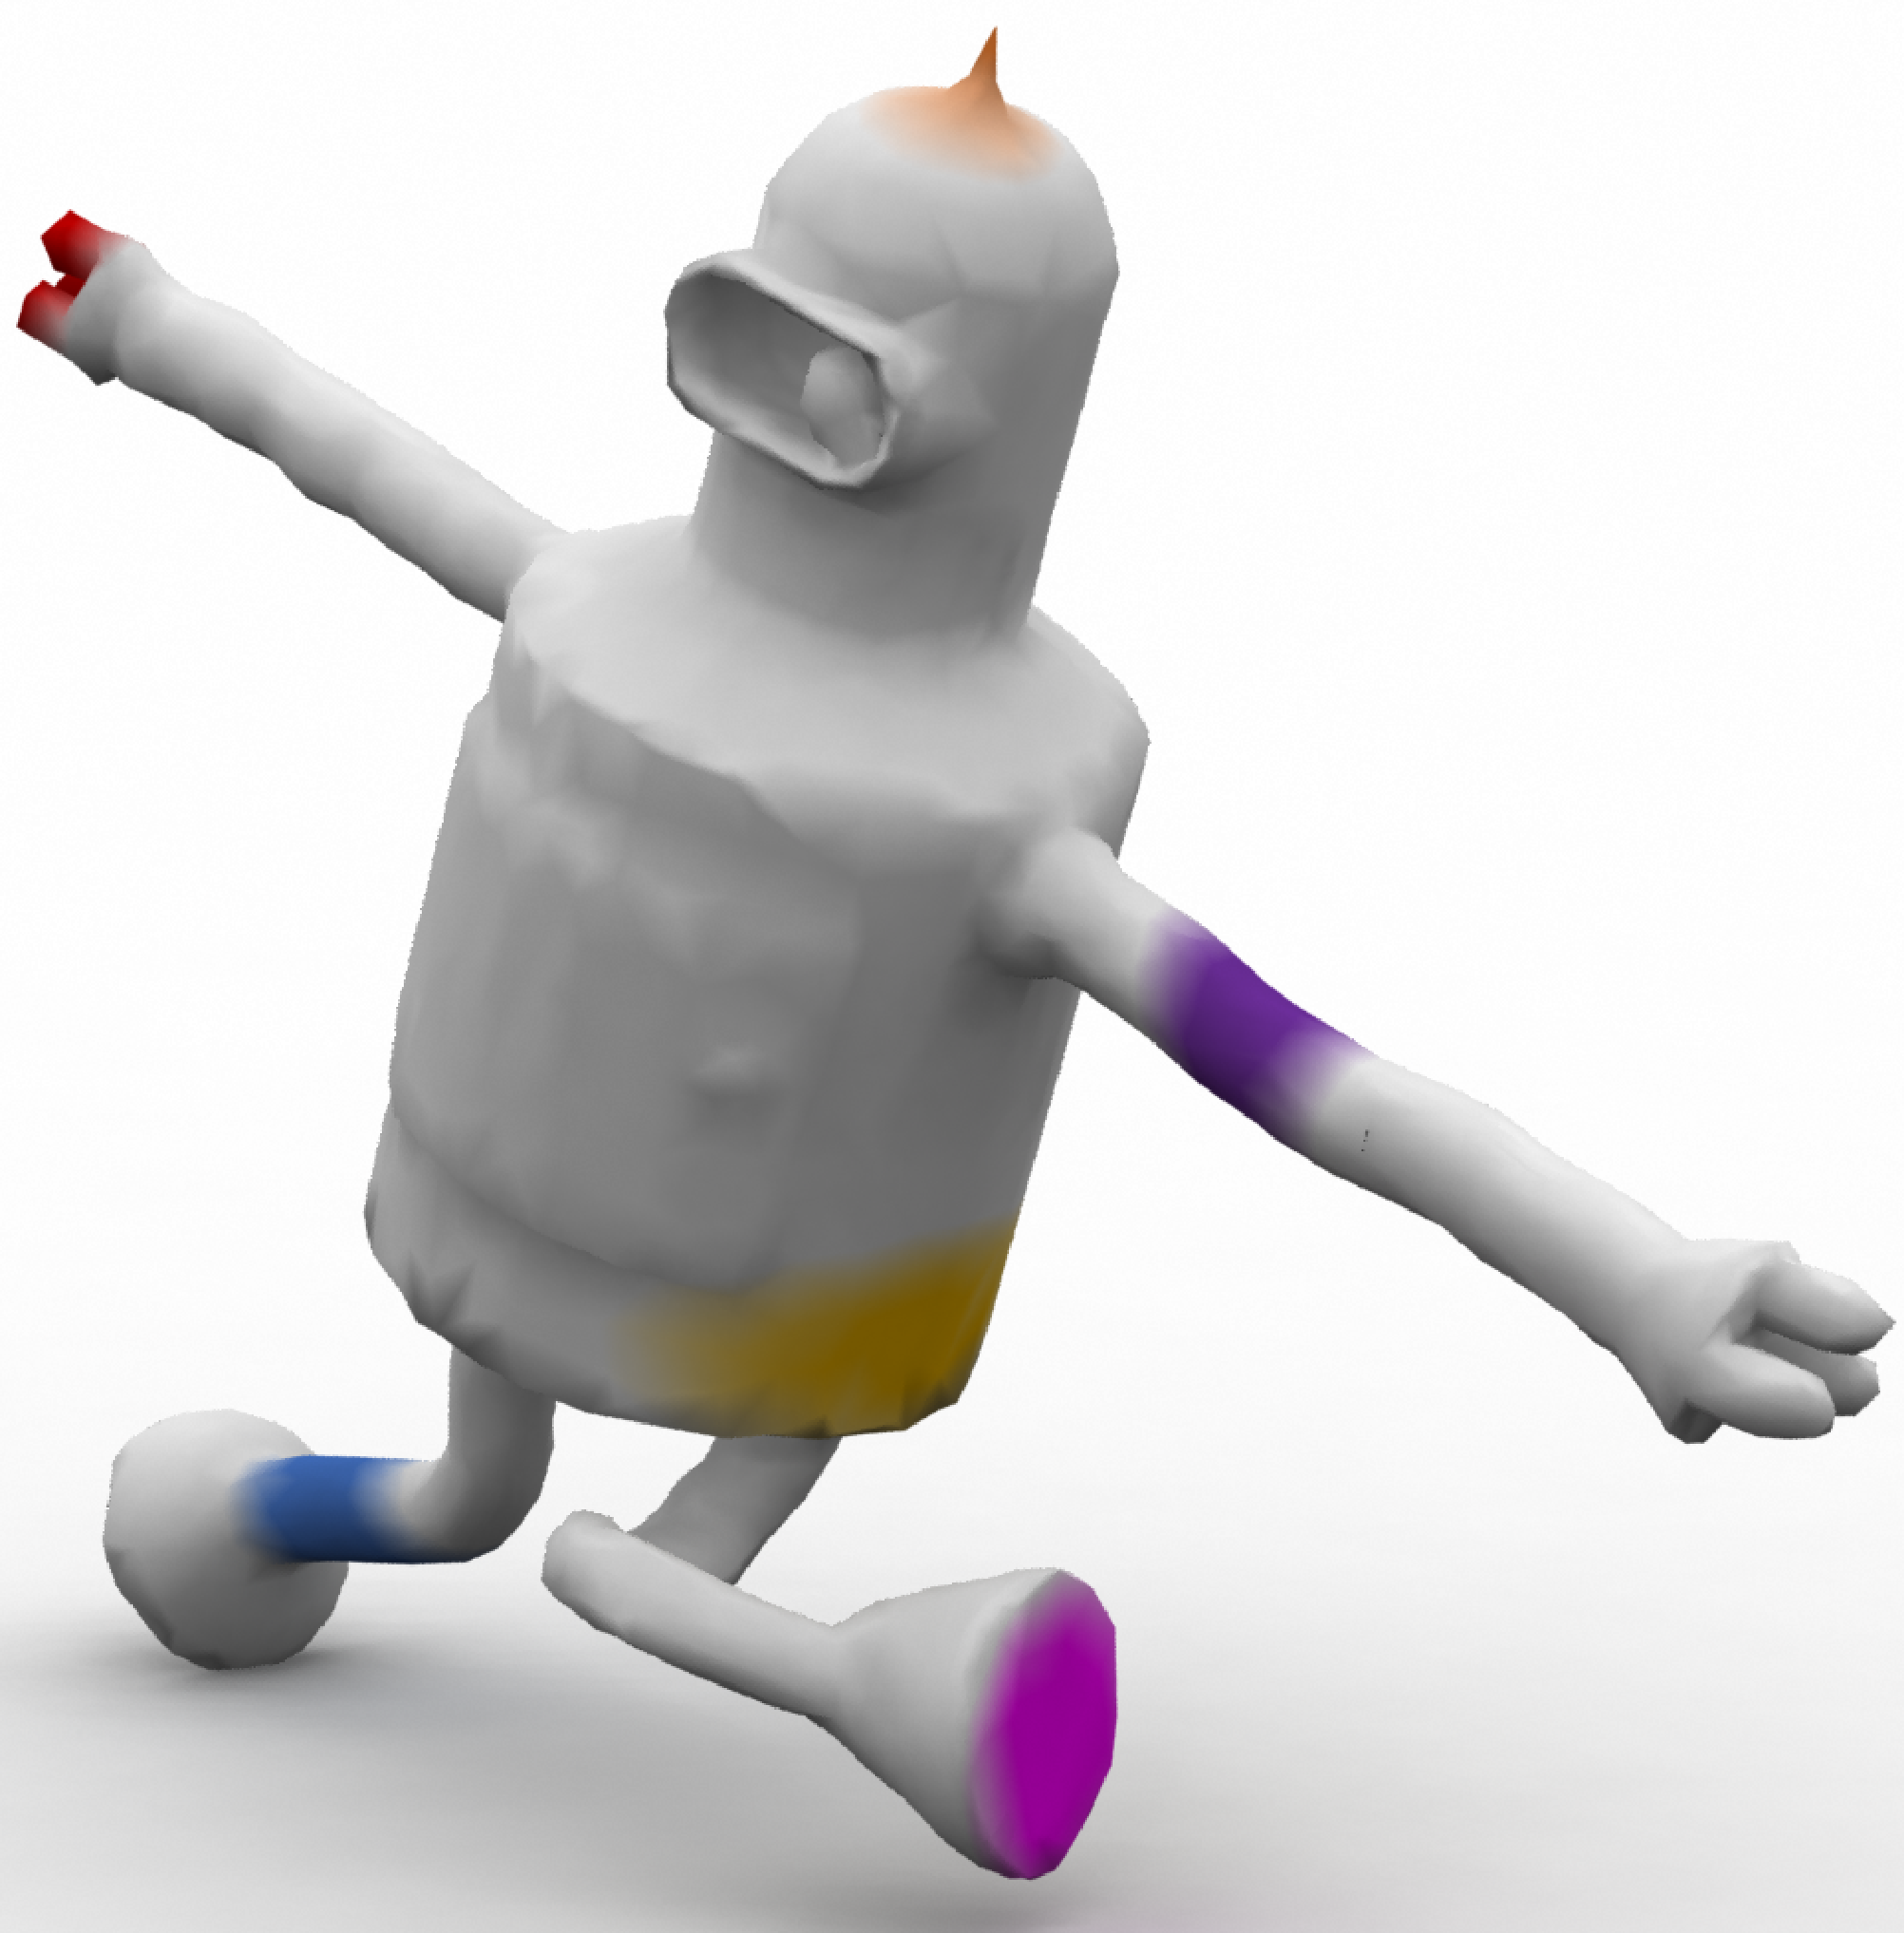
\includegraphics[height=1in]{figures/surface_maps/target_skirt.pdf}&
%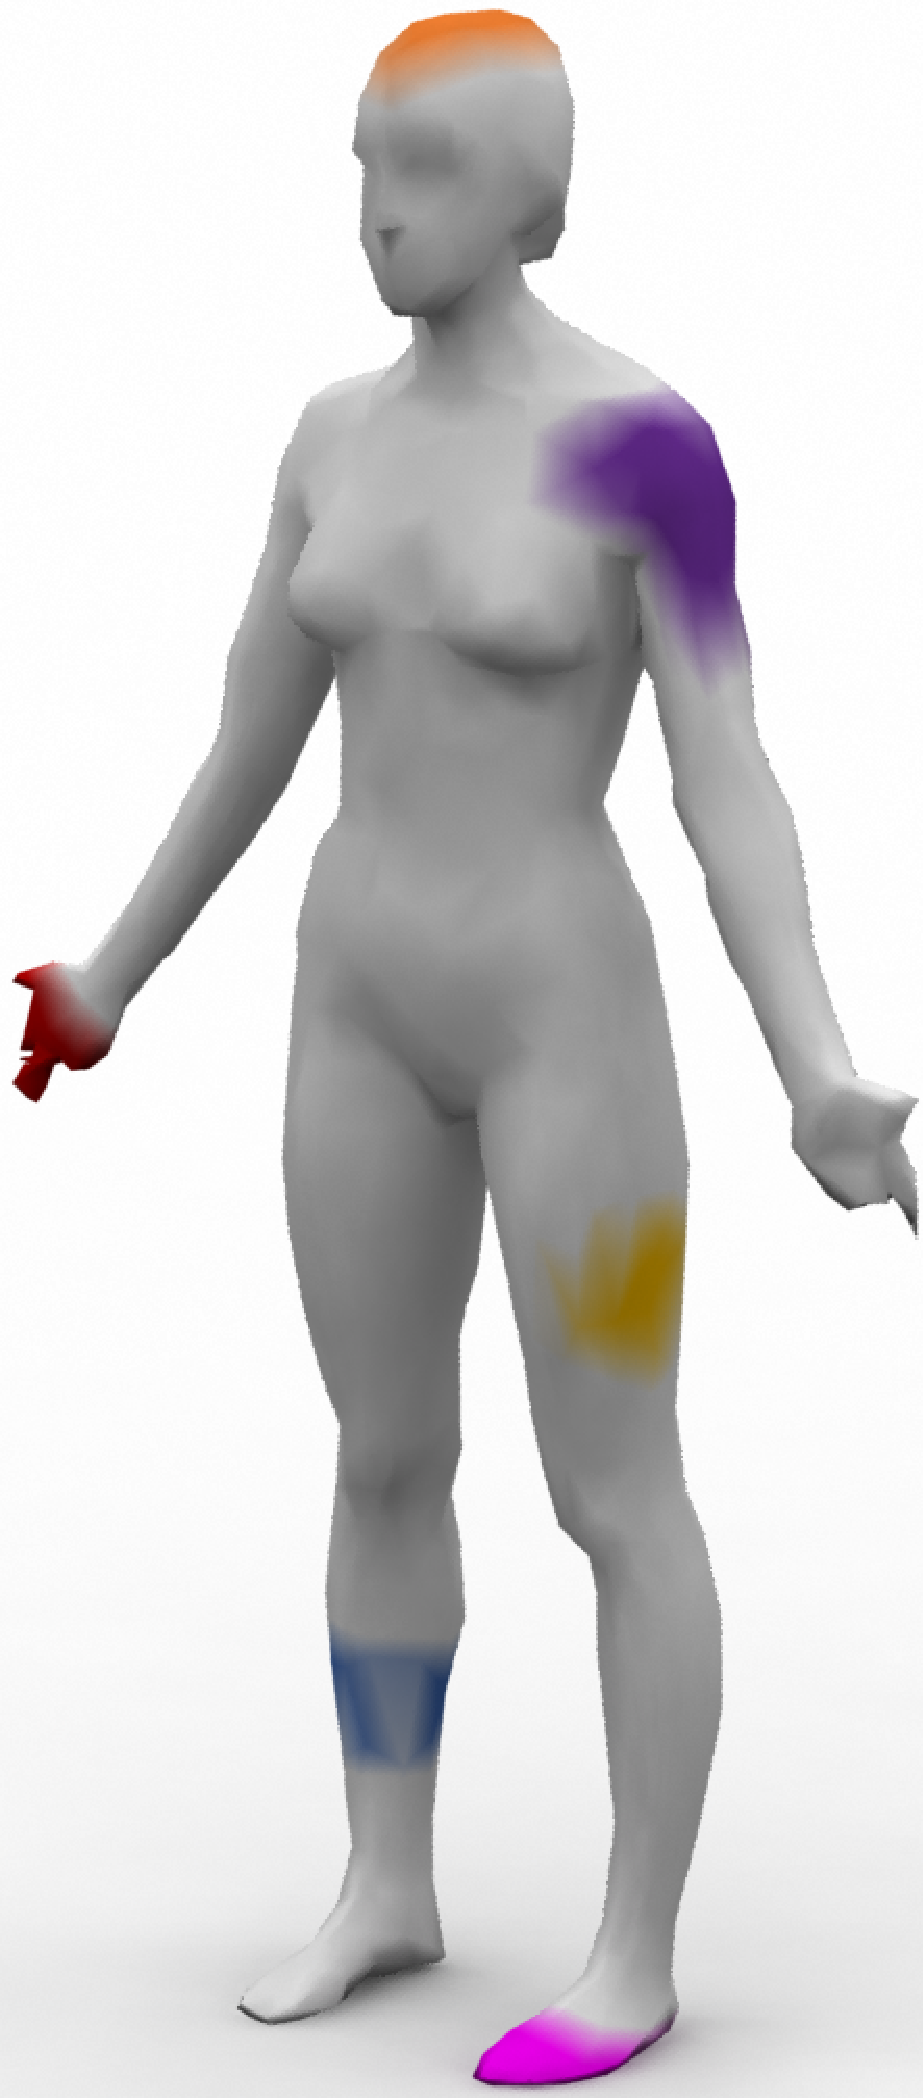
\includegraphics[height=1in]{figures/surface_maps/target_skirt2.pdf}&
%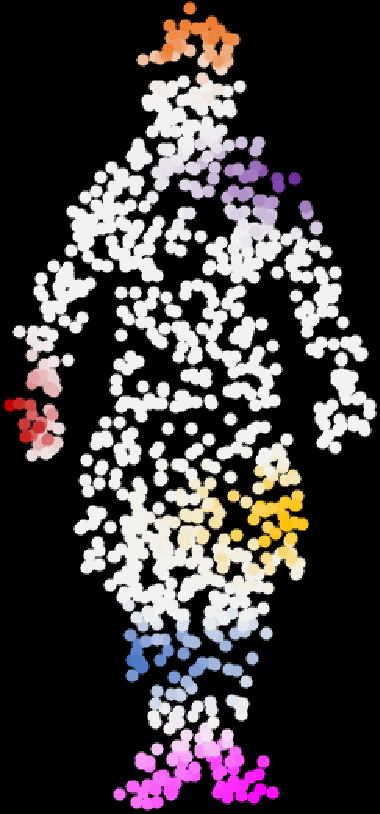
\includegraphics[height=1in]{figures/cloud/cloud2.pdf}&
%\includegraphics[height=1in]{figures/icon/icon_target.pdf}
%\end{tabular}
%\caption{\justin{Write me.}}
}


\maketitle

% !TEX root = ../gw.tex

\begin{abstract}
Many shape and image processing tools rely on computation of correspondences between geometric domains.  Efficient methods that stably extract ``soft'' matches in the presence of diverse geometric structures have proven to be valuable for shape retrieval and transfer of labels or semantic information.  With these applications in mind, we present an algorithm for probabilistic correspondence that optimizes an entropy-regularized  Gromov-Wasserstein (GW) objective. Built upon recent developments in numerical optimal transportation, our algorithm is compact, provably convergent, and applicable to any geometric domain expressible as a metric measure matrix. We provide comprehensive experiments illustrating the convergence and applicability of our algorithm to a variety of graphics tasks. Furthermore, we expand entropic GW correspondence to a framework for other matching problems, incorporating partial distance matrices, user guidance, shape exploration, symmetry detection, and joint analysis of more than two domains.  These applications expand the scope of entropic GW correspondence to major shape analysis problems and are stable to distortion and noise.
\end{abstract}


%%% Local Variables:
%%% mode: latex
%%% TeX-master: "../gw"
%%% End:


%\begin{CRcatlist}
%  \CRcat{I.3.5}{Computer Graphics}{Computational Geometry \& Object Modeling}{Geometric algorithms}
%\end{CRcatlist}

\begin{CCSXML}
<ccs2012>
<concept>
<concept_id>10010147.10010371.10010396.10010402</concept_id>
<concept_desc>Computing methodologies~Shape analysis</concept_desc>
<concept_significance>500</concept_significance>
</concept>
</ccs2012>
\end{CCSXML}

\ccsdesc[500]{Computing methodologies~Shape analysis}

\keywordlist

\conceptlist

\printcopyright

% !TEX root = ../gw.tex

\section{Introduction}

%\gabriel{I found that one thing that is missing, in both abstract/introduction and also a bit in the numerics (put aside partial matching) is that we actually deal with "measured metric spaces". It is a distinctive features from classical matching methods and allows to take into account e.g. some kind of uncertainty in the inputs.}

A basic component of the geometry processing toolbox is a tool for \emph{mapping} or \emph{correspondence}, the problem of finding which points on a target domain correspond to points on a source.  Many variations of this problem have been considered in the graphics literature, e.g.\ with some sparse correspondences provided by the user.  Regardless, the basic task of geometric correspondence facilitates the transfer of properties and edits from one shape to another.

The primary factor that distinguishes correspondence algorithms is the choice of objective functions. Different choices of objective functions express contrasting notions of which correspondences are ``desirable.''  Classical theorems from differential geometry and most modern algorithms consider \emph{local} distortion, producing maps that take tangent planes to tangent planes with as little stretch as possible; slightly larger neighborhoods might be taken into account by e.g.\ aligning heat kernels.  These approaches are justified by classical differential geometry when the matched domains satisfy conditions like near-isometry or near-conformality, but when these conditions are violated these algorithms suffer from having to patch together local elastic terms into a single global map. 

%\suv{Note on style: If possible, avoid using too many gerunds, i.e., ``...ing'' constructions, in favor of directly using verbs; makes the text more readable.}%duly noted!  writing in this paper in part is optimized a bit for space rather than clarity, although that's no excuse for poor exposition :-)

In this paper, we propose a new correspondence algorithm that minimizes distortion of long- and short-range distances alike.  We study an entropically-regularized version of the \emph{Gromov-Wasserstein} (GW) mapping objective function from~\cite{memoli-2011} measuring the distortion of geodesic distances.  The optimizer is a probabilistic matching expressed as a ``fuzzy'' correspondence matrix in the style of~\cite{kim-2012,solomon-2012}; %\gabriel{yes, but at the end of the day, what makes the matrix really fuzzy (at least in the setting where the 2 spaces have the same number of points) is rather the introduction of the entropy. Don't you think ? }
we control sharpness of the correspondence via the weight of an entropic regularizer.   

 Although~\cite{memoli-2011} and subsequent work identified the possibility of using GW distances for geometric correspondence, computational challenges hampered their practical application.  To overcome these challenges, we build upon recent methods for regularized optimal transportation introduced in~\cite{benamou-2015,solomon-2015}.  While optimal transportation is a fundamentally different optimization problem from regularized GW computation (linear versus quadratic matching), the core of our method relies upon solving a sequence of regularized optimal transport problems. %\gabriel{I am not sure the average reader will get the idea. Shouldn't you be more direct and say "resolution of a sequence of simpler regularized optimal transports (i.e. regularized linear programs) comprises ..."}

Our remarkably compact algorithm (see Algorithm~\ref{alg:gw}) exhibits global convergence, i.e., it \emph{provably} reaches a local minimum of the regularized GW objective function regardless of the initial guess.  Our algorithm can be applied to any domain expressible as a metric measure space (see \S\ref{sec:related_work}).  Concretely, only distance matrices are required as input, and hence the method can be applied to many classes of domains including meshes, point clouds, graphs, and even more abstract  structures. 

A major advantage of our framework is its extensibility.  In addition to the conventional correspondence problem, we apply our method to organizing shape collections and show how to find correspondences given user guidance or incomplete pairwise distances.  We also provide algorithms to extract multiple maps in the presence of symmetry and to compute consistent maps within a collection.% via a connection to nonnegative matrix factorization.

%\suv{Is it typical to write this as a para, or can we write out an itemize to make it stand out / be easy for the reviewer?}% I've seen both.  Will change to bullets

\begin{figure}[t]\centering
$
\underbrace{
\includegraphics[height=1in]{figures/icon/icon_source.pdf}
}_{\textrm{Source}}
%\mapsto
\underbrace{
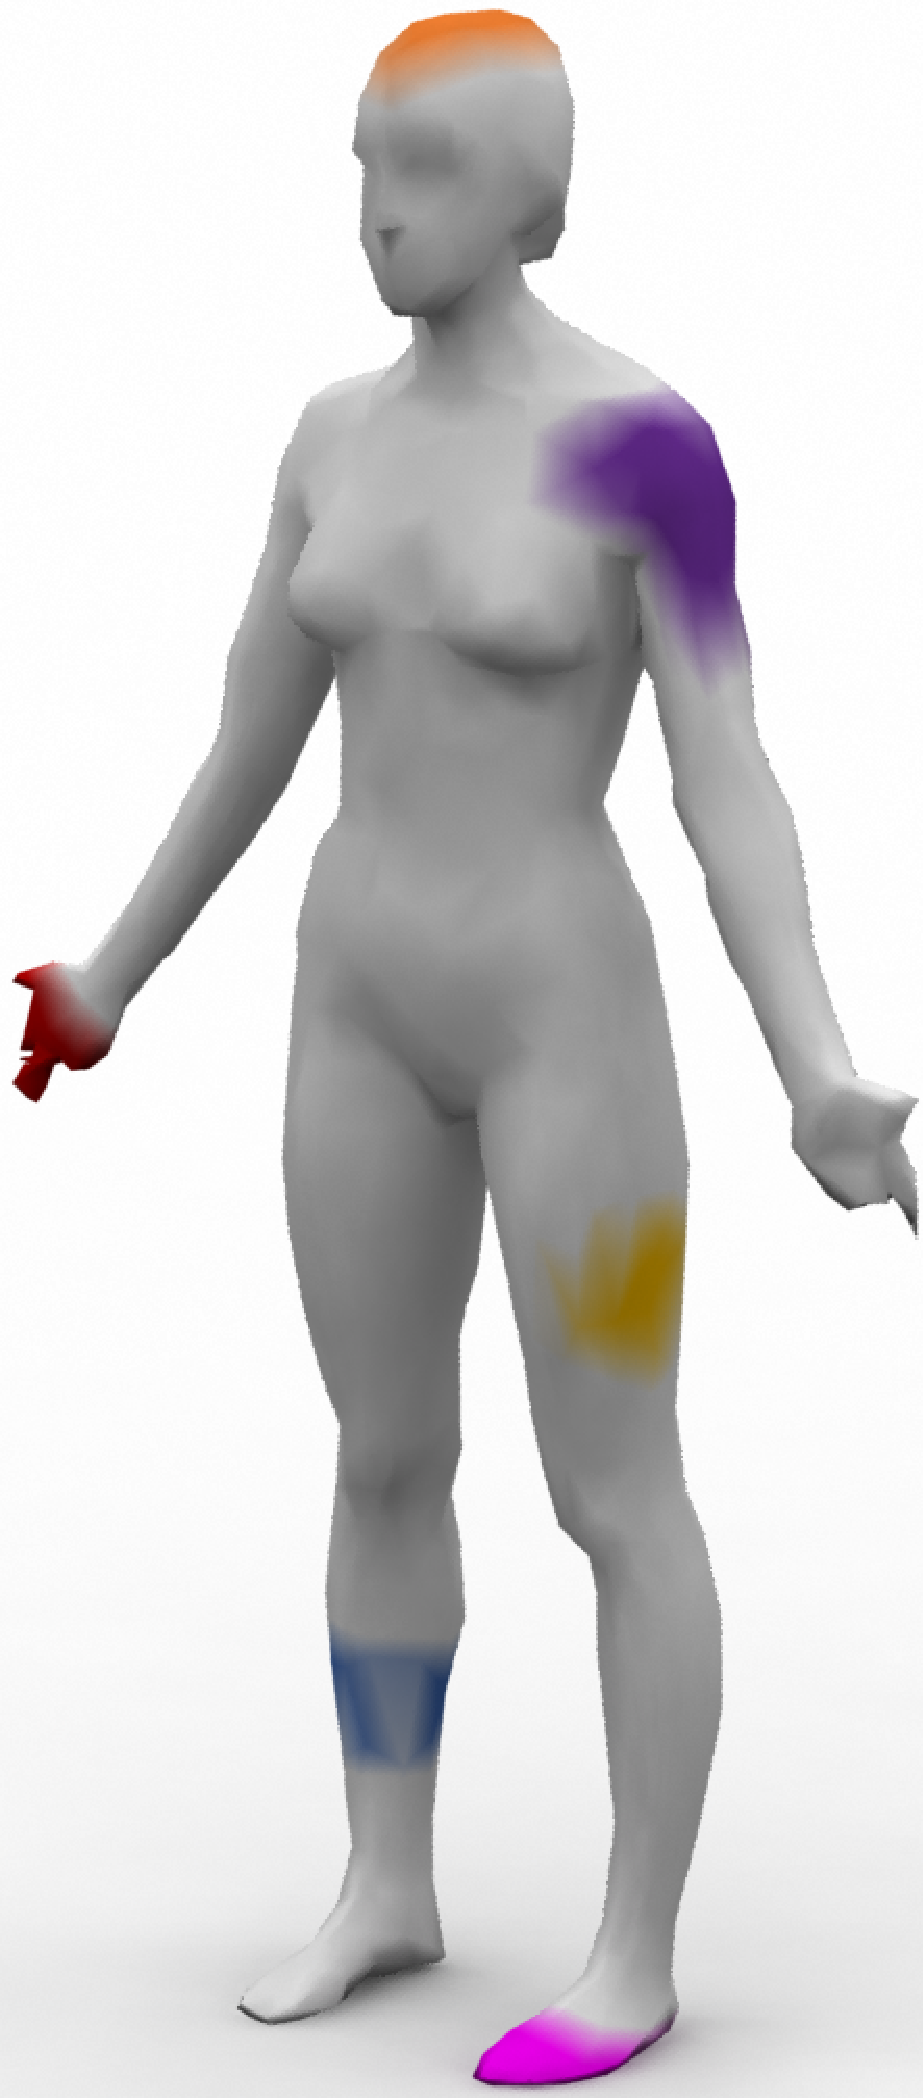
\includegraphics[height=1in]{figures/surface_maps/target_skirt2.pdf}
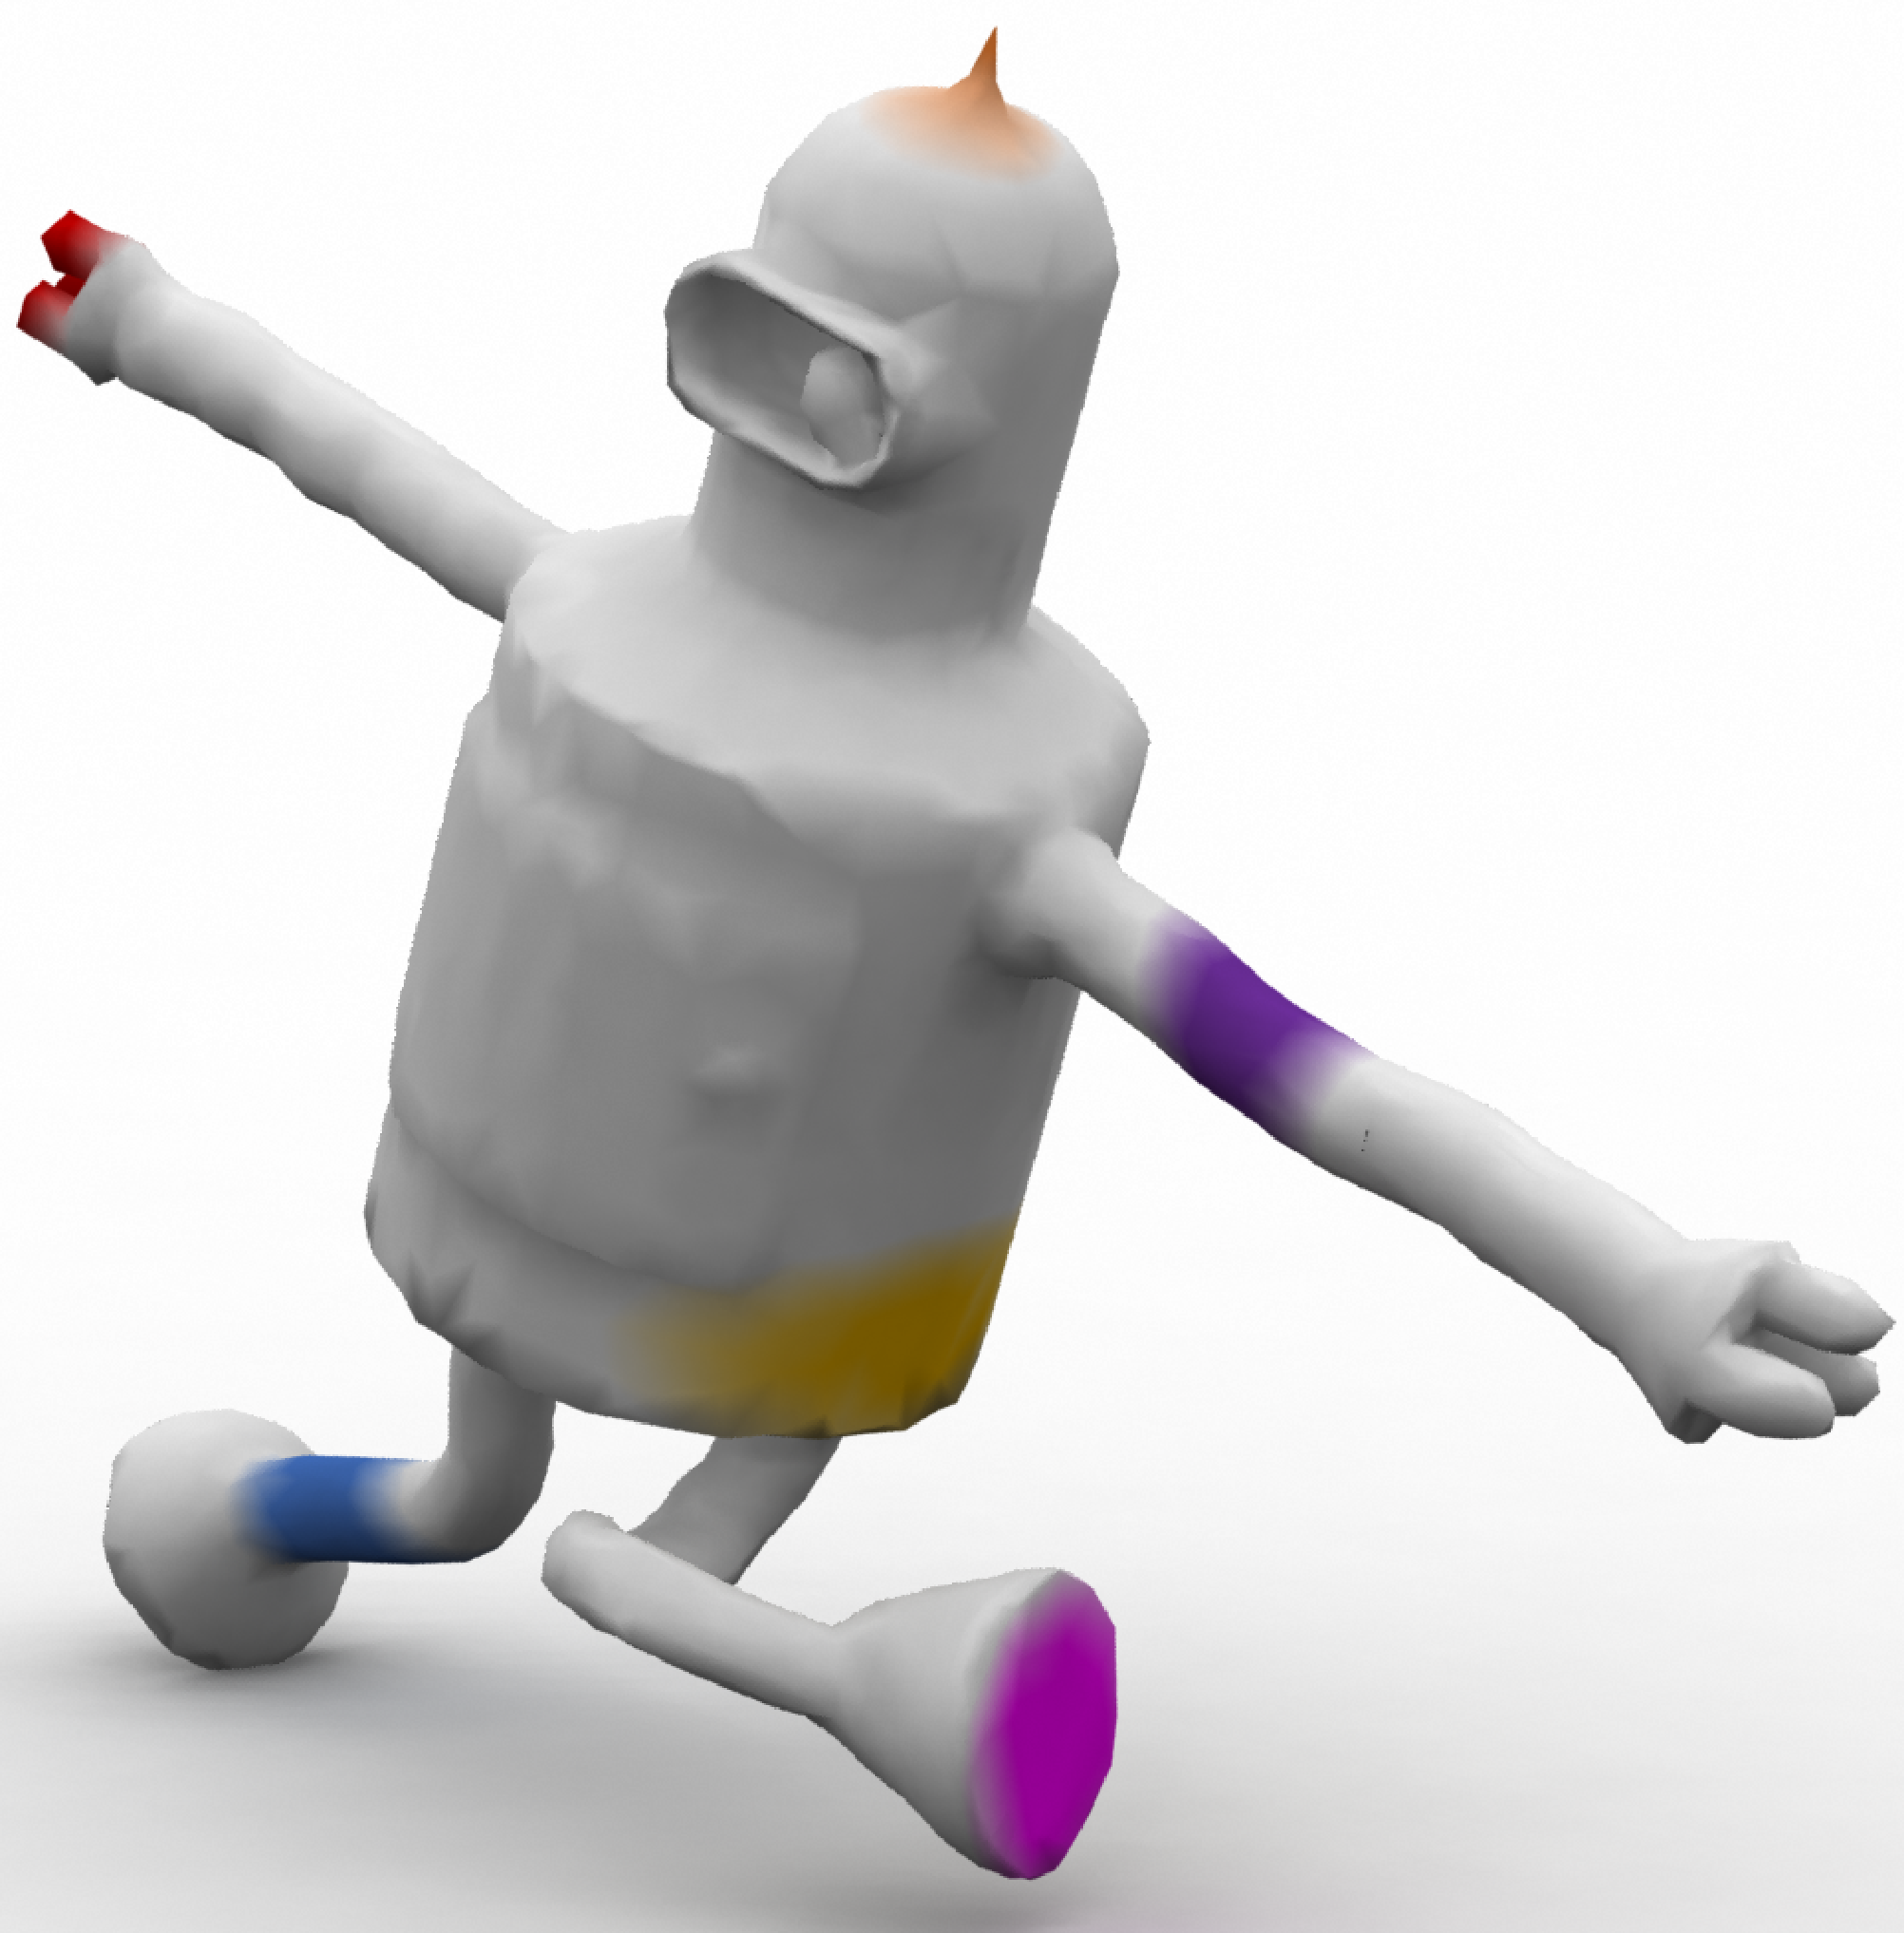
\includegraphics[height=1in]{figures/surface_maps/target_skirt.pdf}
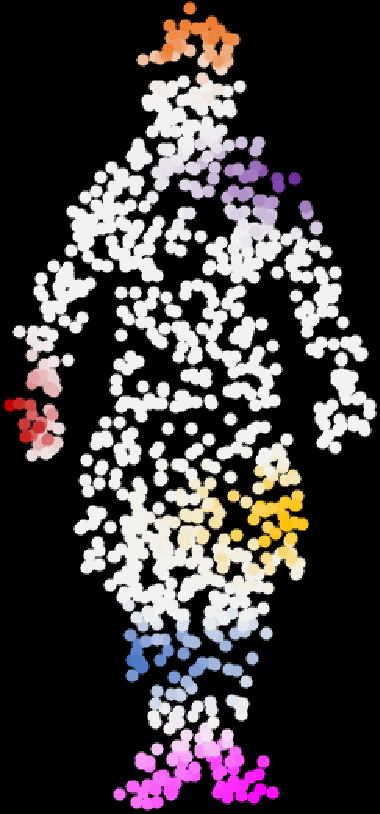
\includegraphics[height=1in]{figures/cloud/cloud2.pdf}
\includegraphics[height=1in]{figures/icon/icon_target.pdf}
\includegraphics[height=1in]{figures/icon/icon_target2.pdf}
}_{\textrm{Targets}}
$
\vspace{-.1in}
\caption{Entropic GW can find correspondences between a source surface (left) and a surface with similar structure, a surface with shared semantic structure, a noisy 3D point cloud, an icon, and a hand drawing. Each fuzzy map was computed using the same code.\vspace{-.2in}}\label{fig:shape_to_icon}
\end{figure}

\paragraph*{Contributions.} We present a fuzzy mapping algorithm minimizing the Gromov-Wasserstein (GW) objective with entropic regularization. In summary, our key contributions are the following: %Specifically, we introduce the following:
\begin{itemize}[topsep=0pt,itemsep=-1ex,partopsep=1ex,parsep=1ex]
\item discretization of an entropically-regularized GW objective suitable for domains in graphics and geometry processing;
\item a simple-to-implement algorithm for minimizing this objective that relies only upon scalable low-level linear algebra;
\item a convergence proof for the iterative optimization algorithm;
\item comprehensive experiments establishing reliability, efficiency, and versatility of the regularized GW algorithm; and
\item proof-of-concept extensions of regularized GW correspondence to a large variety of problems, demonstrating its versatility within the geometry processing and graphics toolboxes.%extensions of regularized GW correspondence to shape exploration, supervised matching, uncertain distance matrices, symmetry detection, and joint domain analysis.
\end{itemize}

%It is simple to implement, applicable to many types of domains, and relies only upon scalable low-level linear algebra.  We provide careful consideration of convergence properties. In addition to evaluating our technique applied to a variety of matching tasks, we show how it can be extended and modified to handle variations of the basic problem, including matching from incomplete distance data and joint domain mapping.
%\justin{to add:  faster than existing fuzzy maps tools}

%\suv{Should related work be Section 1.1 or an entire separate section as of now?}% Usually I've seen SIGGRAPH papers where it's section 2.

% note somewhere --  yaron's sdp for controlling singular values doesn't show it reaches a local min




%Several considerations determine the effectiveness of a technique for correspondence.  From a theoretical standpoint, correspondence algorithms can be judged based on their induced distortion on different classes of shapes, resilience to ambiguity or ill-posedness in the matching problem, and applicability to different geometric representations.  Algorithmic considerations include efficiency or control over the trade-off between accuracy and runtime.  Finally, ease of use, ease of implementation, and the option to provide supervision can make the technique more controllable by an end user.
%
%Countless optimization-based mapping algorithms pose the problem as the minimization of a quadratic objective subject to assorted constraints.  Intuitively, the quadratic term usually measures continuity of the computed map, preferring maps that take nearby points on the source surface to nearby points on the target.  Discrete versions seeking point-to-point maps likely are algorithmically intractable---even within a constant approximation factor~\cite{sahni-1976}---and after relaxing integer constraints the problem remains similarly intractable~\cite{sahni-1974}.
%
%For this reason, quadratic correspondence techniques generally either work with a convexification of the original problem or lack convergence guarantees or global optimality.  The former approach has gained popularity due to the possibility of proving guarantees on the quality of the output and/or certificates of optimality, at the expense of having to solve large-scale convex problems that severely limit the number of matched points~\cite{solomon-2013,kezurer-2015}.  Furthermore, these relaxations can have large convex hulls of optimal solutions when the mapping problem admits even a discrete symmetry.  Contrastingly, simpler heuristic approaches to mapping might be considered approximations to the original nonconvex problem with few guarantees.
%
%In this paper, we bridge between these extremes with a mapping algorithm for the original nonconvex mapping problem that is straightforward to implement using simple and relatively efficient iterations.  Despite its simplicity, the algorithm is \emph{provably} convergent to a critical point of the objective regardless of the initial guess, and the convergence rate appears to be sufficient for practical use.
%
%In particular, we propose algorithms for optimizing a regularized version of the \emph{Gromov-Wasserstein} objective seeking maps between surfaces that preserve pairwise geodesic distances; in the absence of isometry, this objective promotes minimal distortion of the geodesic structure of the domain.  While this approach to matching was proposed in~\cite{memoli-2011}, the underlying numerical problem presented significant challenges that led to the proposal of aggressive spectral approximations that are far more sensitive to deviation from isometry~\cite{memoli-2009}.
%
%Furthermore, we extend our technique to computation of consistent maps within a collection.  We propose a completely unsupervised pipeline incorporating consistency into the mapping pipeline rather than enforcing it \emph{a posteriori}.  Our approach is made possible via a connection to nonnegative matrix factorization (NMF) techniques appearing in the machine learning literature.
%
%We demonstrate our computational techniques on a variety of computational techniques, including not only shape matching but also \justin{TBD.}
%
%\paragraph*{Contributions.} \justin{Write me last.}


%%% Local Variables:
%%% mode: latex
%%% TeX-master: "../gw"
%%% End:

% !TEX root = ../gw.tex

\section{Related Work}\label{sec:related_work}

Our algorithm is a general technique for mapping, a problem that has a long history in graphics. In this section, we focus on works relevant to our discussion; see~\cite{kaick-2011} for a thorough survey of correspondence algorithms.

%TODO:  Conformal wasserstein distances

\paragraph*{Gromov-Wasserstein (GW) distances.}  

We focus on the GW mapping objective~\cite{memoli-2007}, a relaxation of the Gromov-Hausdorff (GH) distance between metric spaces~\cite{gromov-2001}. GH measures the single distance most distorted by a map.  While it has been applied to geometry processing~\cite{bronstein-2010}, GH is costly to optimize and prioritizes one distance value at a time.%; \cite{bronstein-2010} apply it to geometry processing.

%\gabriel{Tentative of new paragraph}

GW is a distance between \emph{metric measure spaces}, i.e., metric spaces equipped with a probability distribution (see~\cite{memoli-2011,memoli-2014,SturmGW} for more details). This additional feature is crucial, especially because it allows one to measure the \emph{expected} distortion of distances. Matchings considered by GW distances thus differ from the point-to-point maps considered by Gromov-Hausdorff distances. GW distances optimize over probabilistic ``measure couplings'' (see \S\ref{sec:matching}), the continuous counterpart of ``fuzzy'' mapping matrices introduced in~\cite{kim-2012,solomon-2012}.
% 
Using an additional probability distribution on a metric space is also beneficial from an application point of view, because one can encode additional information (such as spatially varying confidence or noise level) in the probability distribution; see \S\ref{sec:weighted_mtx} for an example.

%\gabriel{this is the old paragraph}

%GW distances measure the \emph{expected} distortion of distances.
%See~\cite{memoli-2011,memoli-2014} for discussion, and~\cite{SturmGW} for theoretical developments. % on GW distances.

%The representation of a map for GW distances also differs from the point-to-point map considered in constructing Gromov-Hausdorff distance.  GW distances optimize over probabilistic ``measure couplings'' (see \S\ref{sec:matching}), the continuous counterpart of ``fuzzy'' mapping matrices introduced in~\cite{kim-2012,solomon-2012}.


\paragraph*{Mapping objectives.} Most mathematical methods for correspondence are built around criteria for a desirable map, expressed in algorithmic design choices or as terms in an objective function.  Here, we attempt to place GW distances in this larger context.

%\suv{Aren't the kernelized methods below limited to matching symmetric matrices, which on top must also be positive definite? Thus, the ``convexity'' versus ``non-convexity'' concern also applies here?}

Many mapping methods attempt to minimize \emph{local} distortion, measuring the stretch of the source onto the target.  In differential geometry, harmonic maps minimize a local measure of stretch and shear~\cite{urakawa-2013}.  Heat kernel-based methods like~\cite{ovsjanikov-2010} prefer maps that distort local distances and curvatures; Kezurer et al.~\shortcite{kezurer-2015} use a similar objective.  ``Kernelized sorting''~\cite{quadrianto-2009} optimizes the Hilbert Schmidt Independence Criterion~\cite{smola-2007}, which coincides with the GW objective function after replacing geodesic distances with diffusion kernels. Fried et al.~\shortcite{fried-2015} apply this machinery to image layout problems.  These methods are subject to the challenge of assembling many local constraints into one map.

%GW distances belong to a different class of methods, which seek maps that preserve global geometric structure.  
Other mapping methods seek to preserve global structure.  Bronstein et al.~\shortcite{bronstein-2006} showed that one such objective is effective for nonrigid mesh registration, optimized using simple gradient-based steps; Aflalo and Kimmel~\shortcite{aflalo-2013} introduce a spectral approximation in the presence of a Laplacian operator for machine learning applications.  These methods can make it difficult to localize points in small neighborhoods but are well-suited to fuzzy mapping applications.  Our regularized GW mapping technique belongs to this class but is accompanied by a more stable optimization routine than its peers.

If more is known about the mapped geometry, specialized algorithms may apply.  For instance, Kim et al.~\shortcite{kim-2011} seek nearly conformal maps between surfaces and Wei et al.~\shortcite{wei-2015} train for maps between human body models.  Chen and Koltun~\shortcite{chen-2015} rely on extrinsic alignment to reduce matching ambiguity for triangulated surfaces.  We aim to devise a versatile method that does not depend on these assumptions, making it applicable to many domains (see \S\ref{sec:experiments}).

Our measure couplings bear some rough similarity to the functional map matrices of Ovsjanikov et al.~\shortcite{ovsjanikov-2012}, but the underlying variables are different.  We minimize geometric distortion, while they use weaker ``commutativity'' regularizers and descriptors.  Functional map matrices in the Laplace-Beltrami basis also can take on negative values, which are explicitly avoided in our probabilistic formulation.

\paragraph*{Optimal transportation.}  As we will see in \S\ref{sec:matching}, the GW matching objective function inherits part of its name from the Wasserstein distance between probability distributions on a geometric domain.  These latter distances have recently been applied to several problems in graphics; a small sampling includes~\cite{bonneel-2011,degoes-2011,merigot-2011,deGoes-2012,schwartzburg-2014,solomon-2014,deGoes-2015,solomon-2015}. Despite this relationship, the Wasserstein and GW distances serve contrasting purposes and require different computational machinery.

%\gabriel{I am not a big fan of underline, I would prefer italic.}\justin{This is a strategic underline :-) --- you'll see I used italics everywhere else.  I'm really worried lazy SIGGRAPH reviewers will quickly write this off as an easy extension of last year's paper.  So, I used unexpected typography to make them read this sentence twice :-)}

%\suv{I guess the first sentence below is also 'strategic' because it otherwise essentially repeats the message of the last sentence of the previous paragraph. Also, what if you use \textbf instead of underline? maybe that is too annoying.}
GW and Wasserstein distances apply to different problems.  Wasserstein distances are between distributions on the \underline{same} geometric domain.  GW distances are between \underline{different} geometric domains.  From an optimization standpoint, Wasserstein distances are defined by a convex linear program~\cite{villani-2003,rubner-2000}, while GW distances require solving a nonconvex quadratic program. % This makes it impossible to apply Wasserstein algorithms directly to the GW case.

%\gabriel{I would insist on the fact that it is in large the entropy that leads to fuzzy coupling. }\justin{Added a sentence to the next paragraph}

Nonetheless, we leverage algorithms for Wasserstein distances as building blocks.  We apply entropic regularization, proposed for optimal transportation in~\cite{cuturi-2013,benamou-2015} and introduced to graphics in~\cite{solomon-2015}; the entropic Sinkhorn algorithm comprises our inner loop.  Our algorithm resembles ``softassign'' in machine learning~\cite{rangarajan-1997} (see \S\ref{sec:convergence}).  The entropic term controls the fuzziness of our coupling; highly-regularized problems can generate meaningful rough maps in just a few iterations, while decreasing the regularizer better approximates the GW problem at the cost of more expensive optimization.

%\suv{Do we need any comparison with Memoli's approach?}%oddly, Memoli doesn't provide many details about his approach, algorithmically at least.  The BFGS comparison is my best guess --- he mentions approximate Hessians...

\paragraph*{Quadratic assignment and correspondence.}  GW computation is an instance of the quadratic assignment problem~\cite{pardalos-1994,loiola-2007,cela-2013}.  Solving this problem with global optimality and point-to-point constraints likely is algorithmically intractable---even within a constant approximation factor~\cite{sahni-1976}.  After relaxing integer constraints the problem remains similarly intractable~\cite{sahni-1974}.

%\suv{Any word on how our approach fits in given the difficulty of quadratic assignment. I would place this para before the optimization para to end the related work on a more positive note, also because that refers to the stuff we actually use.}% no idea theoretically --- i would imagine the most general case of GW with arbitrary D matrices is equivalent to general quadratic assignment

\paragraph*{Optimization.}  Limited attention has been dedicated to the problem of computing GW distances efficiently.  Initial work used general-purpose solvers.  M\'emoli~\shortcite{memoli-2009} introduces a spectral approximation bounded by solving a sequence of linear programs.  

An alternative approach with theoretical guarantees is convex relaxation, removing constraints from nonconvex problems until they become convex programs.  %\suv{What is tightness theory?} 
Some theoretical results provide conditions under which these methods recover a global optimum for the original problem, that is, when the relaxations are \emph{tight}.  While the potential for global optimality is attractive, the number of relaxed variables can be huge.  For instance, Kezurer et al.~\shortcite{kezurer-2015} optimize over $n^2\times n^2$ semidefinite matrices, where $n$ is the number of mapped points, and~\cite{solomon-2012,solomon-2013} include many large-scale transportation subproblems.  Furthermore, relaxed problems with non-unique solutions, e.g.\ mapping in the presence of symmetries, admit large spaces of unusable outputs.  See~\cite{aflalo-2014,aflalo-2015,lyzinski-2015} for similar trade-offs in graph matching.  Eigenvalue relaxations, e.g.~\cite{leordeanu-2005}, also provide some notion of global optimality, with much less favorable conditions for tightness and after removing many constraints.

Our algorithm instead inherits convergence and \emph{local} optimality from recent work on nonconvex optimization~\cite{bot-2015}.  It resembles a discretized gradient flow in the Kullback-Leibler (KL) metric, similar to the forward--backward proximal gradient algorithm~\cite{bauschke-2011,combettes-2011} extended to Bregman divergences~\cite{bauschke-2006}.  Guarantees for nonconvex objectives come from the Kurdyka-{\L}ojasiewicz (also KL) property~\cite{kurdyka-1998,lojasiewicz-1963,lojasiewicz-1993}, applied to nonconvex optimization by Attouch et al.~\shortcite{attouch-2010}.



%%% Local Variables:
%%% mode: latex
%%% TeX-master: "../gw"
%%% End:

% !TEX root = ../gw.tex

\section{Matching a Pair of Domains}\label{sec:matching}

\subsection{Gromov-Wasserstein Matching}\label{sec:gw_matching}

Suppose we are given two geometric domains $\source$ and $\target$ accompanied with %\gabriel{I would replace ``unit measure'' by ``probability measure'' to indicate they are positive}� \justin{I avoided ``probability'' here because people I asked to read it were confused about the difference between GW and Wasserstein. I added "nonnegative," hopefully this is enough.}
nonnegative unit measures $\mu_0$ and $\mu$, resp.  Following~\cite{memoli-2011}, define the space $\M(\mu_0,\mu)$ of \emph{measure couplings} as the set of measures $\gamma\in\Prob(\source\times \target)$ satisfying
$$\gamma(S_0\times \target)=\mu_0(S_0)\textrm{\ \ \  and\ \ \ }\gamma(\source\times S)=\mu(S)$$
for all measurable $S_0\subseteq\source$ and $S\subseteq\target.$  We will treat $\gamma$ as a ``soft correspondence'' in the language of~\cite{solomon-2012}, that is, a high probability assigned by $\gamma$ to $(p_0,p)\in\source\times\target$ indicates that $p_0$ and $p$ should be matched.

To add geometric structure, assume $\source$ and $\target$ are additionally accompanied with pairwise distance functions $d_0:\source\times\source\rightarrow\R_+$ and $d:\target\times\target\rightarrow\R_+$.  The \emph{2-Gromov-Wasserstein} (GW) distance between $(\mu_0,d_0)$ and $(\mu,d)$ measures the minimal distortion induced by a measure coupling between the two domains:
\begin{equation}\label{eq:smooth_gw}
\begin{array}{l}\displaystyle
\GW_2^2((\mu_0,d_0),(\mu,d))\eqdef\\
\displaystyle
\hspace{.1in}
\min_{\gamma\in\M(\mu_0,\mu)}\iint_{\source\times\target} 
\hspace{-.2in}
\left[
d_0(x,x')\!-\!d(y,y')
\right]^2
d\gamma(x,y)\,d\gamma(x',y').
\end{array}
\end{equation}
In contrast to optimal transportation, this optimization is a potentially nonconvex \emph{quadratic program} rather than a linear program due to the product of two $d\gamma$'s.  

The GW objective is constructed from the assumption that if a map pairs $x\mapsto y$ and $x'\mapsto y'$, then the distance between $x$ and $x'$ on $\source$ should be similar to the distance between $y$ and $y'$ on $\target$.  If $d$ is the geodesic distance function, then the objective is zero when $\gamma$ encodes an isometry between $\source$ and $\target$.  That said, $\gamma$ is meaningful even when $\source$ and $\target$ are not isometric, measuring the optimal deviation from preserving the distance structure of a surface.

%\gabriel{I am sure we already spoke about this, but why do not use the constraint $\G\1=\bmu_0$ instead of $\G\bmu=\1$, and directly define the objective as  $\sum_{ijk\ell} (\D_{0ij}\!-\!\D_{k\ell})^2 \G\!_{ik}\G\!_{j\ell}\bmu_{0i}\bmu_{0j}$ ? This would seems more natural and match the continuous definition, no? }%see email chain....

While our subsequent derivation could be written in continuous language, for clarity and to focus on computational applications we transition to discrete notation.  Assume $\source$ is discretized using $n_0$ points and that $\target$ is discretized using $n$ points; we accompany these samplings with discrete measures $\bmu_0\in\R_+^{n_0}$ and $\bmu\in\R_+^n$ such that $\1^\top\bmu_0=\1^\top\bmu=1.$  In our experiments, we take $\bmu_0,\bmu$ either to be constant vectors or---for triangle meshes---vectors of per-vertex barycentric area weights; future work might consider more general choices of these vectors.  We use symmetric matrices $\D_0\in\R_+^{n_0\times n_0}$ and $\D\in\R_+^{n\times n}$ to denote pairwise distances on $\source$ and $\target$.  

In this language, the set of  measure couplings is 
\begin{equation}\label{eq:couplings}
\bM(\bmu_0,\bmu)\!\eqdef\!\{\G\in\R^{n_0\times n}_+\!:\!\G\bmu=\1,\G^\top\bmu_0=\1\},
\end{equation}
and the 2-Gromov-Wasserstein distance is
\begin{equation}\label{eq:GW2}
\bGW_2^2(\D_0,\!\D)\!\eqdef\!\min_{\G\in\bM} \sum_{ijk\ell} (\D_{0ij}\!-\!\D_{k\ell})^2\G\!_{ik}\G\!_{j\ell}\bmu_{0i}\bmu_{0j}\bmu_k\bmu_\ell.
\end{equation}
We think of $\G$ as a function sampled from $\source\!\times\!\target$, so the products $\G^\top\bmu_0$ and $\G\bmu$ integrate out $\source$ and $\target$, resp.  The linear constraints defining $\bM$ reflect the fact that $\G$ should marginalize to the constant probability measure on $\source$ and $\target$.

Define an inner product of measure couplings as
$$\langle\G,\G'\rangle\eqdef\sum_{ik} \G\!_{ik}\G\!_{ik}' \bmu_{0i}\bmu_k.$$
After expanding the square, we can write
\begin{equation}\label{eq:GW2_inner_prod}
\bGW_2^2(\D_0,\!\D)\!=\!
2\min_{\G\in\bM}\langle \G, \bL(\G)\rangle,
\end{equation}
where
$$
\bL(\G)\!\eqdef\!
\frac{1}{2}\D_0^{\wedge2}\diag{\bmu_0}\G\bmu\1^\top
\!-\!\D_0\diag{\bmu_0}\G\diag{\bmu}\D
\!+\!\frac{1}{2}\1\bmu_0^\top \G\diag{\bmu}\D^{\wedge2}.
$$
The superscript $\wedge2$ denotes the elementwise square of a matrix, and $\diag{\v}$ is the diagonal matrix constructed from vector $\v$.

Applying the marginalization constraints~\eqref{eq:couplings} shows 
\begin{equation}\label{eq:discrete_optim_noreg}
\bGW_2^2(\cdot)
\!=\!
C(\D_0,\D)
\!-\!
2\max_{\G\in\bM} 
\langle \G,\D_0\diag{\bmu_0}\G\diag{\bmu}\D\rangle,
%\sum_{ijk\ell}\D_{0ij}\D_{k\ell}\G\!_{ik}\G\!_{j\ell} \bmu_{0i}\bmu_{0j}\bmu_k\bmu_\ell,
\end{equation}
where
$$C(\D_0,\D)\eqdef\sum_{ij}\D_{0ij}^2\bmu_{0i}\bmu_{0j} + \sum_{k\ell}\D_{k\ell}^2\bmu_k\bmu_\ell.$$
This maximization problem for $\G$ %has two drawbacks.  First, it 
is a nonconvex quadratic program for $\G,$ removing the possibility of using convex optimization tools.  Any time $\source$ or $\target$ admit a symmetry, the objective has multiple optima, one for each symmetry.  For example, when mapping human models, the two optima will be the orientation-preserving map and a left-to-right flipped map.  Unlike convex relaxations, however, a convex combination of the orientation-preserving and orientation-reversing maps will \emph{not} necessarily be optimal.

% \suvrit{Actually, the doubly stochastic set of matrices is what makes this nonconvex problem tricky. Ultimately, the nonnegativity constraints of \bM are what make this difficult.}

\subsection{Entropic Regularization}\label{sec:entropic_reg}

%\suv{In the same spirit as $\mapsto$ Following}
Following~\cite{solomon-2015}, we define the \emph{entropy} of a measure coupling as
$$H(\G)\eqdef -
\langle \G,\ln\G\rangle,
$$
%\sum_{ik} \bmu_{0i}\bmu_k\G\!_{ik}\ln\G\!_{ik},$$
$H(\G)$ is large when $\G$ has many nonzero entries and is small when $\G$ encodes a map close to a permutation matrix.  

\begin{figure*}[t]\centering
\begin{tabular}{c|c|c}
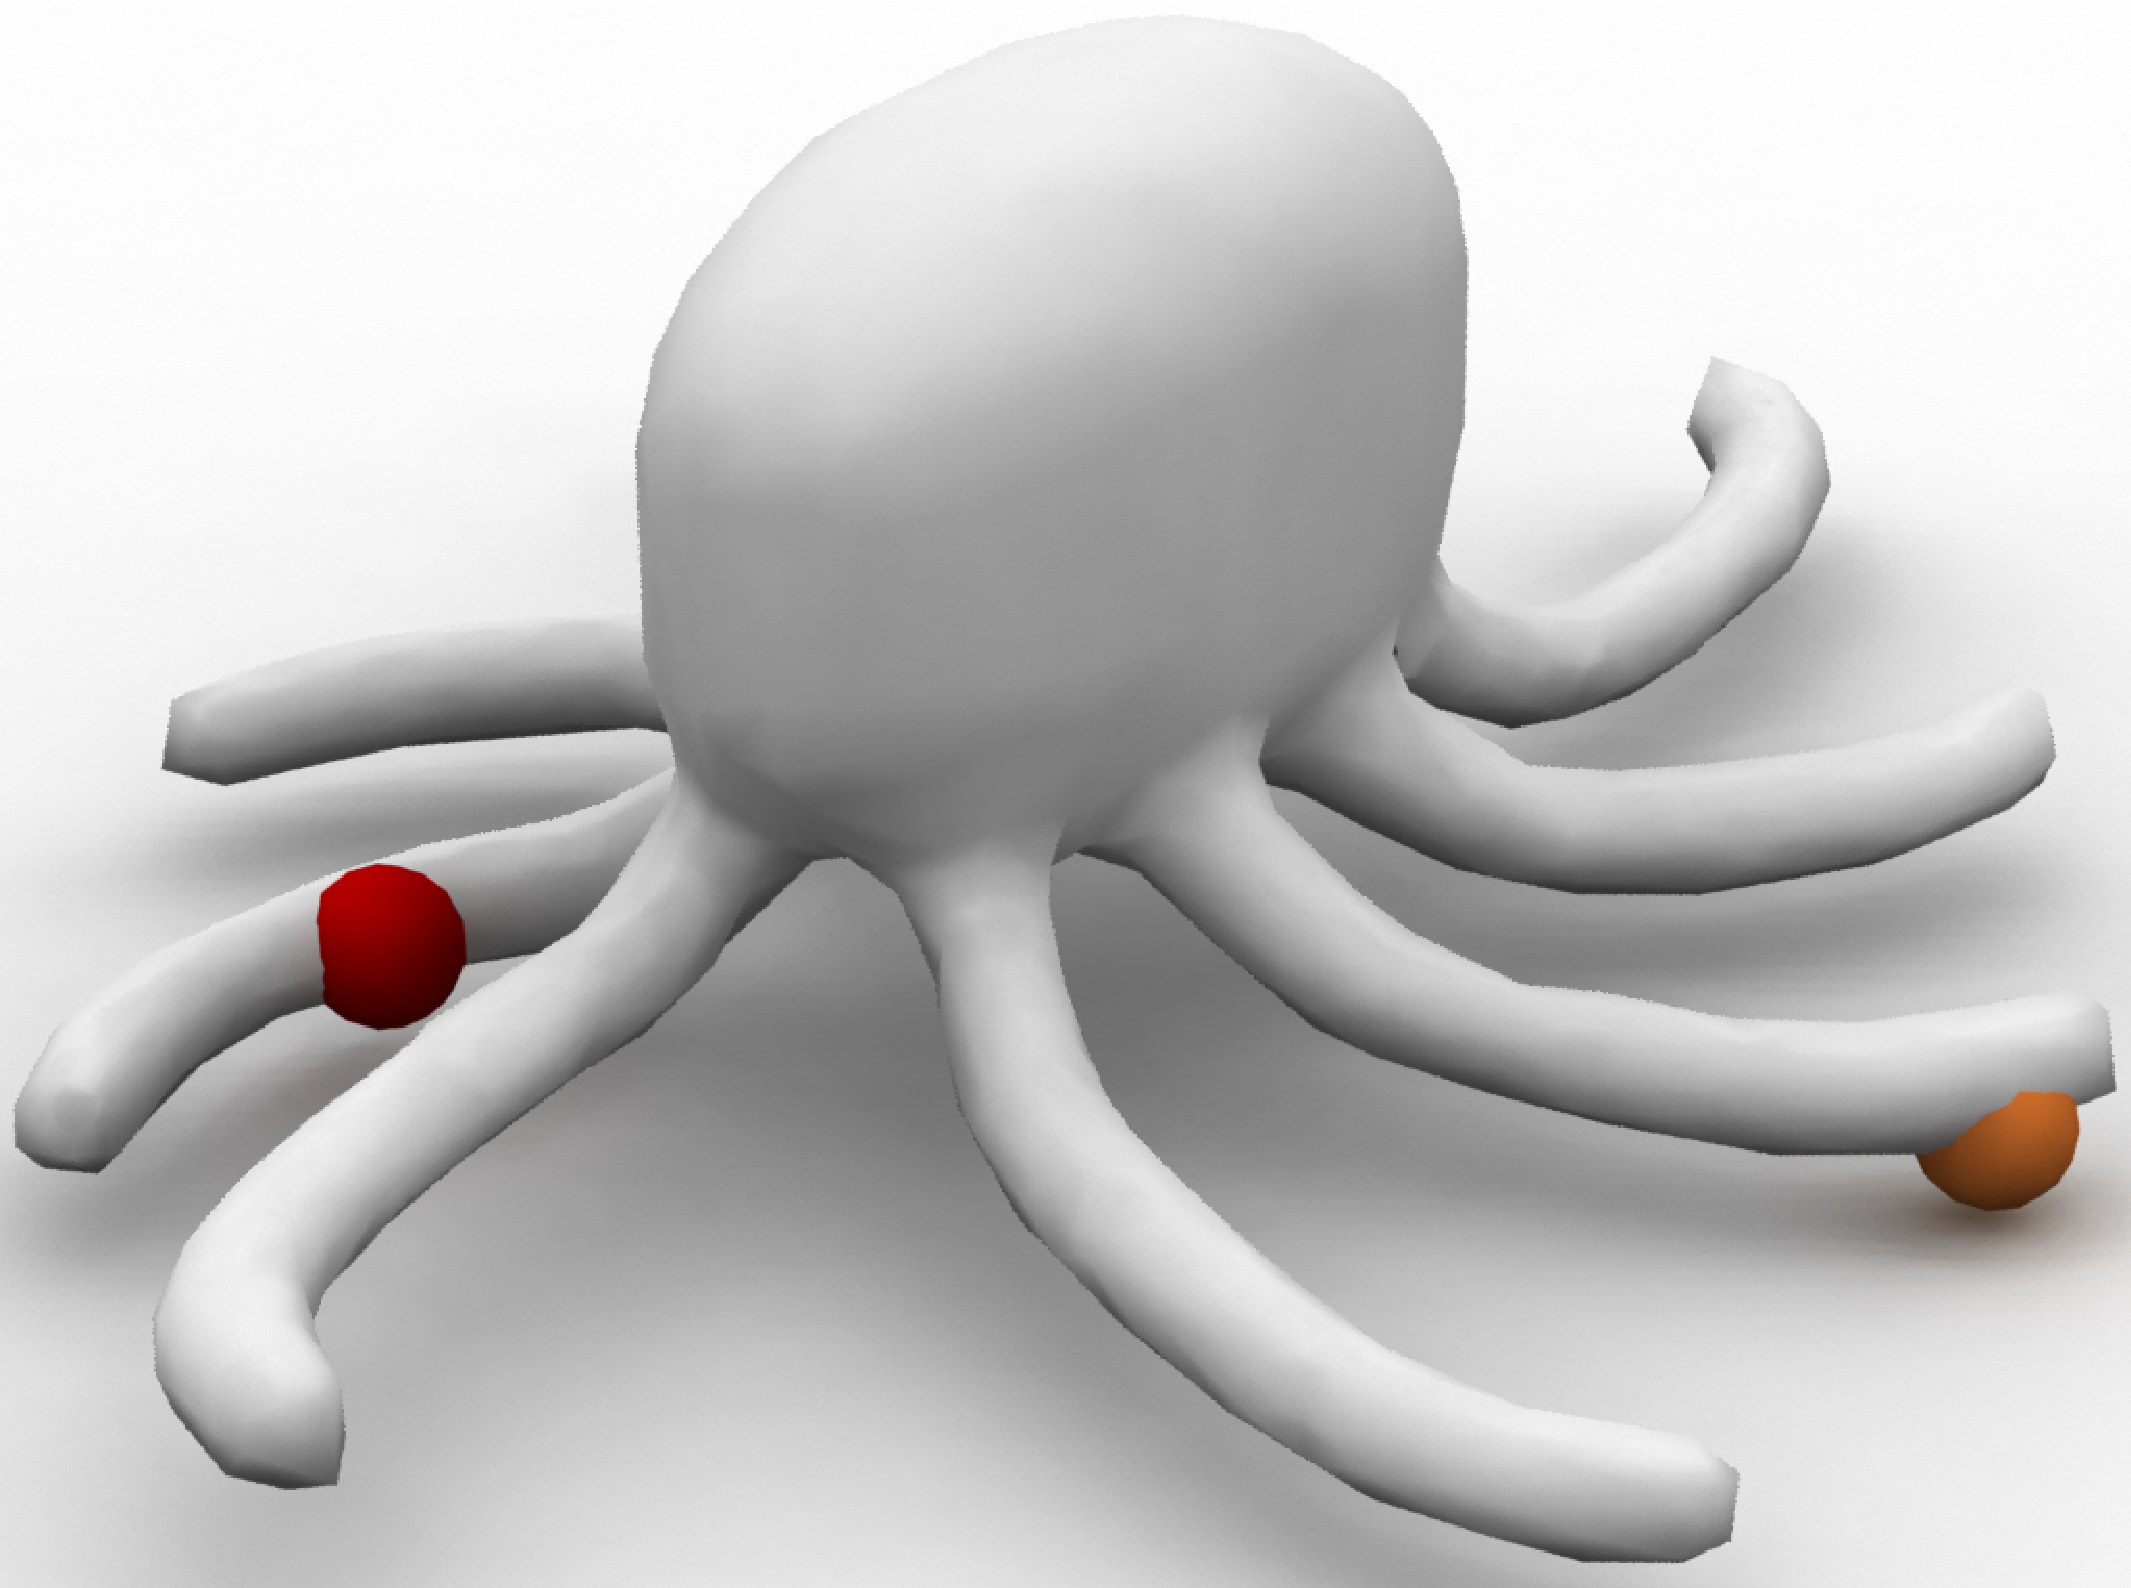
\includegraphics[height=.16\linewidth]{figures/regularization/source_octopus.pdf} &
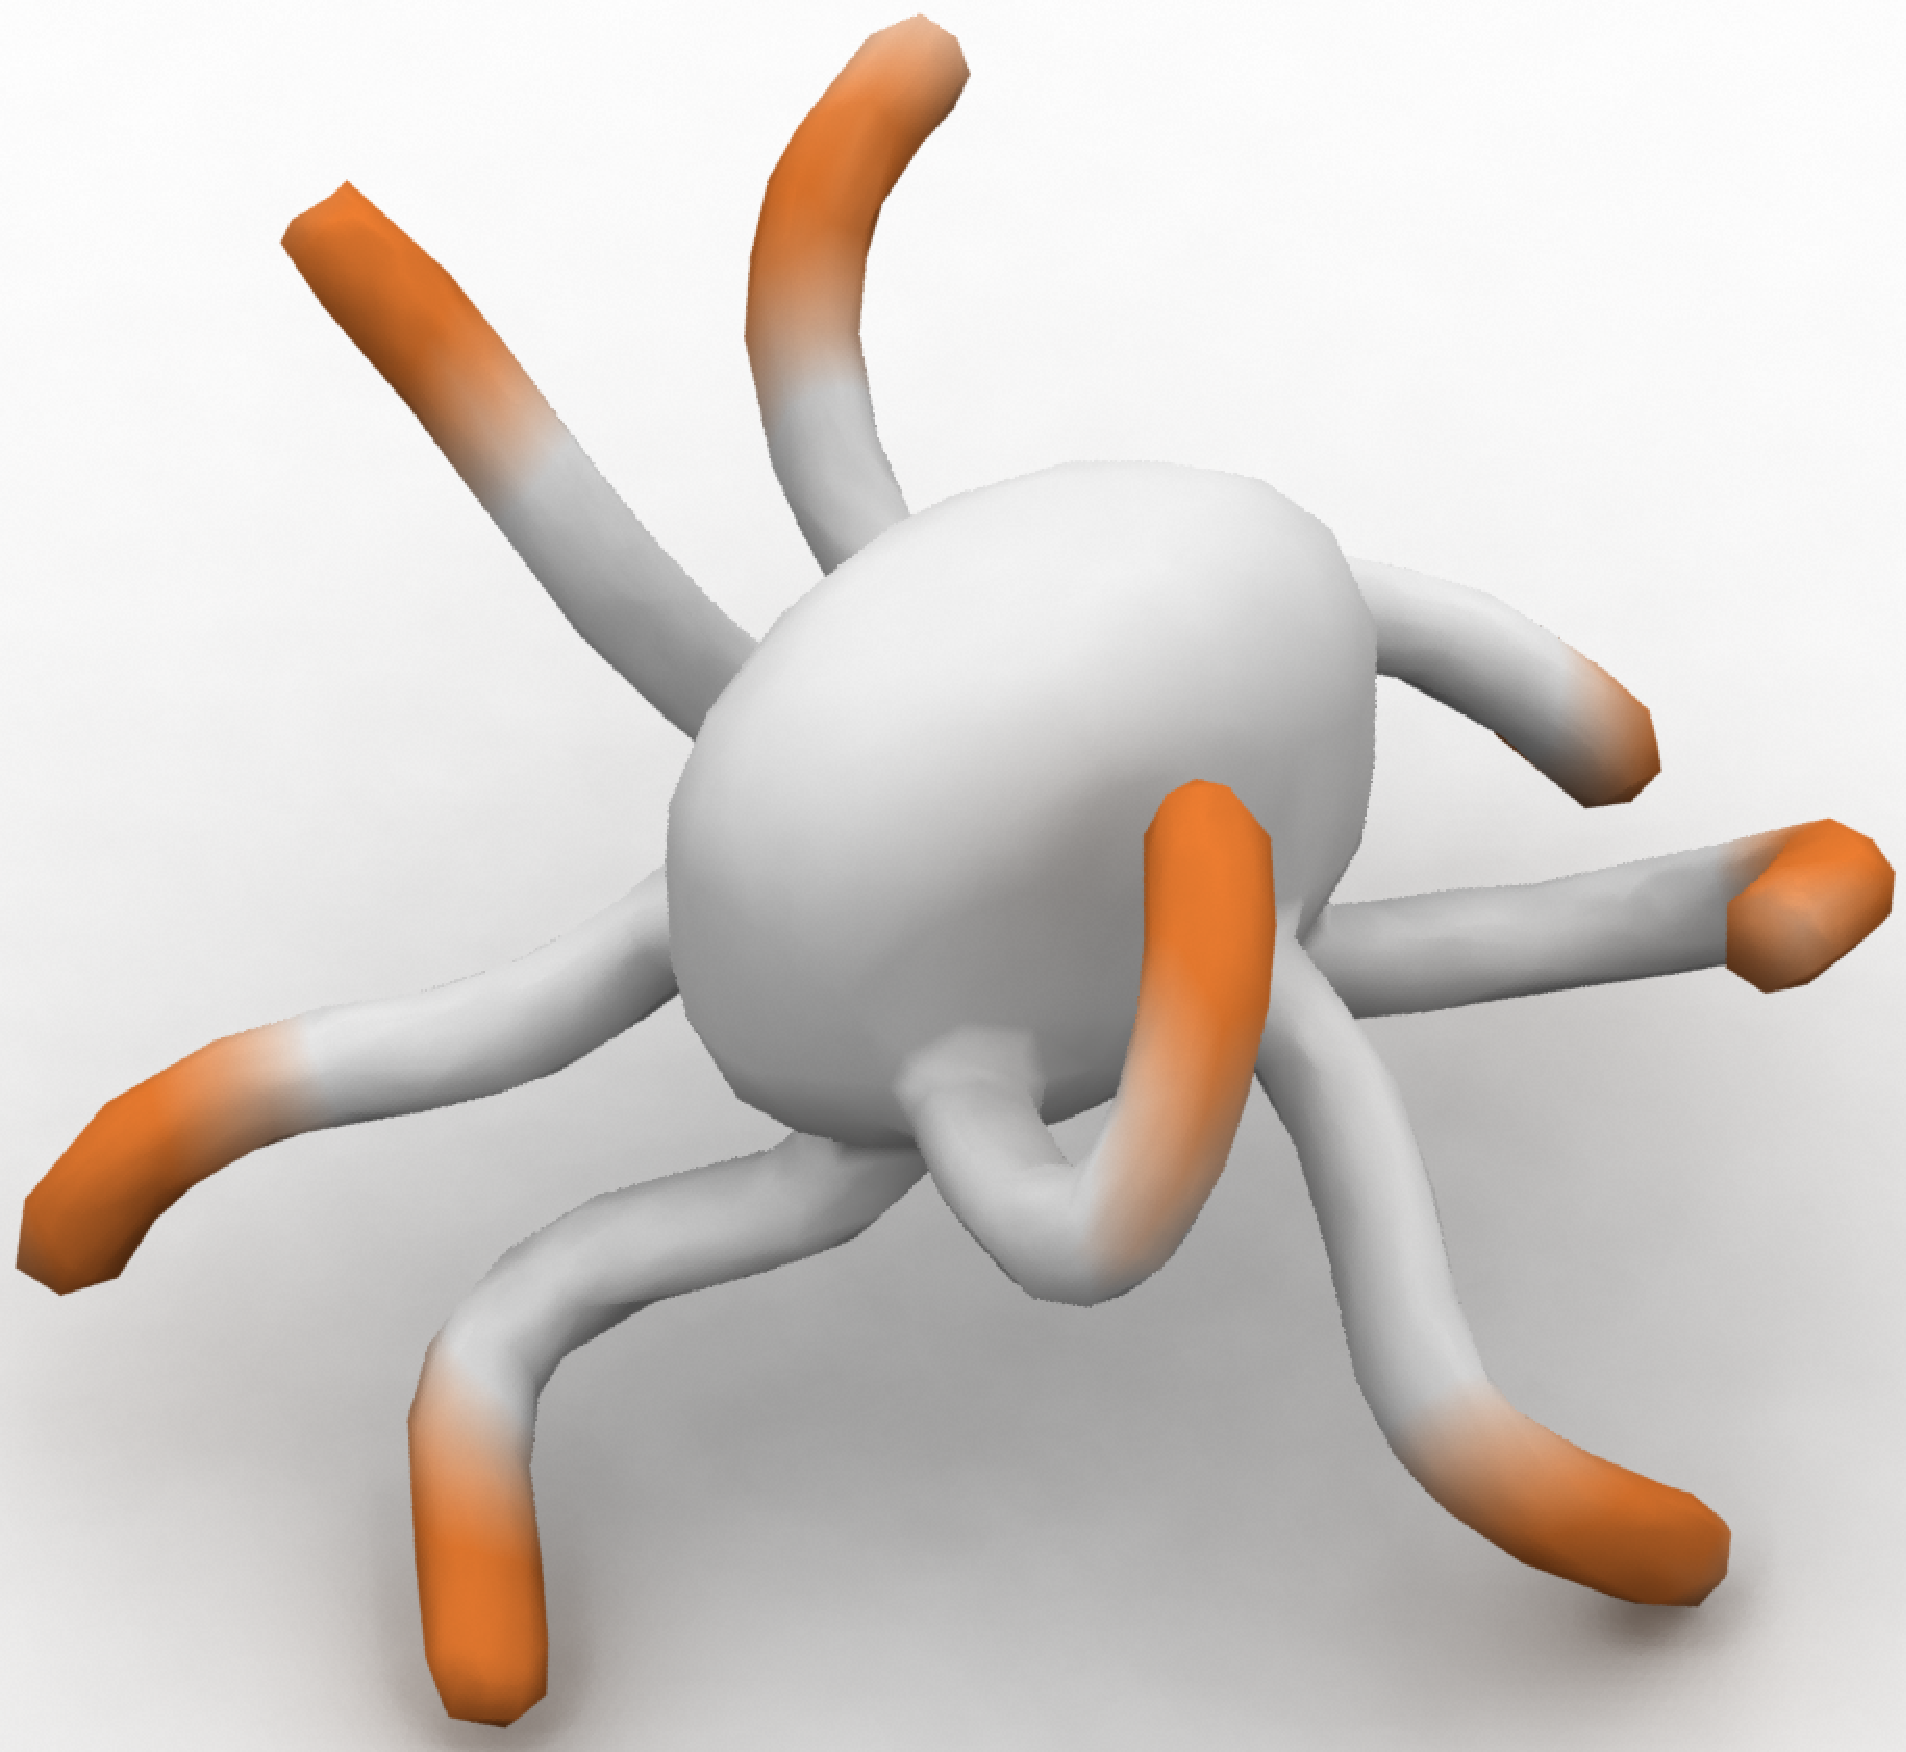
\includegraphics[height=.16\linewidth]{figures/regularization/target_octopus1_0.008.pdf}
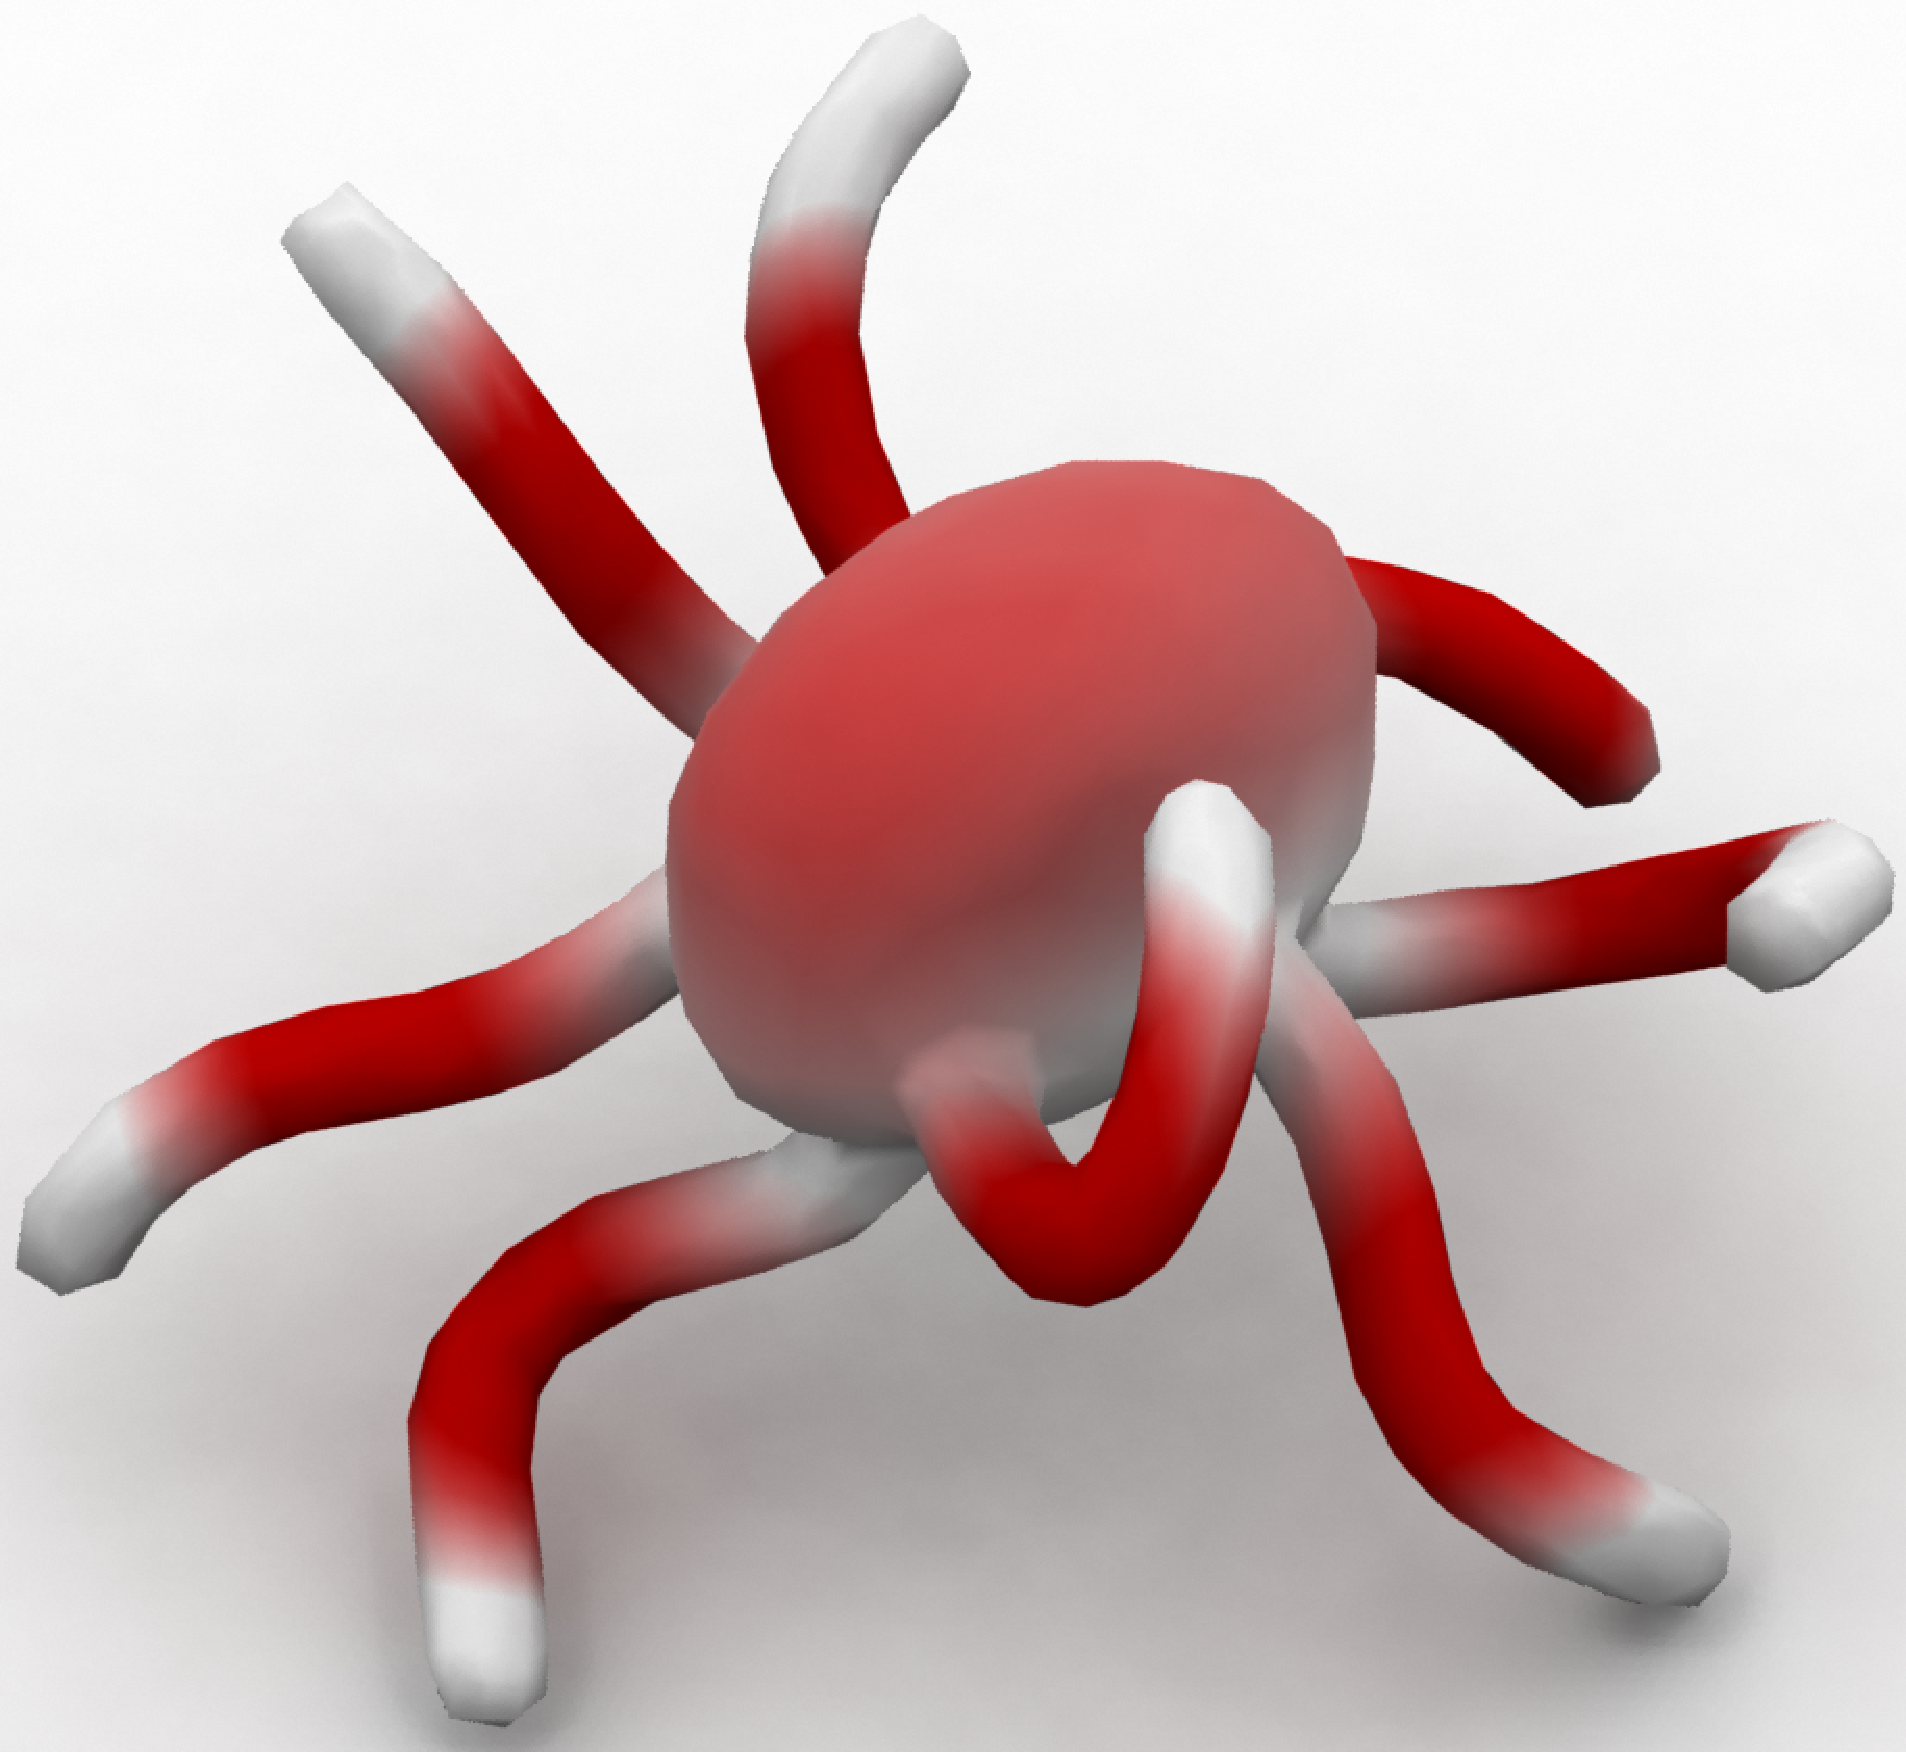
\includegraphics[height=.16\linewidth]{figures/regularization/target_octopus2_0.008.pdf}
&
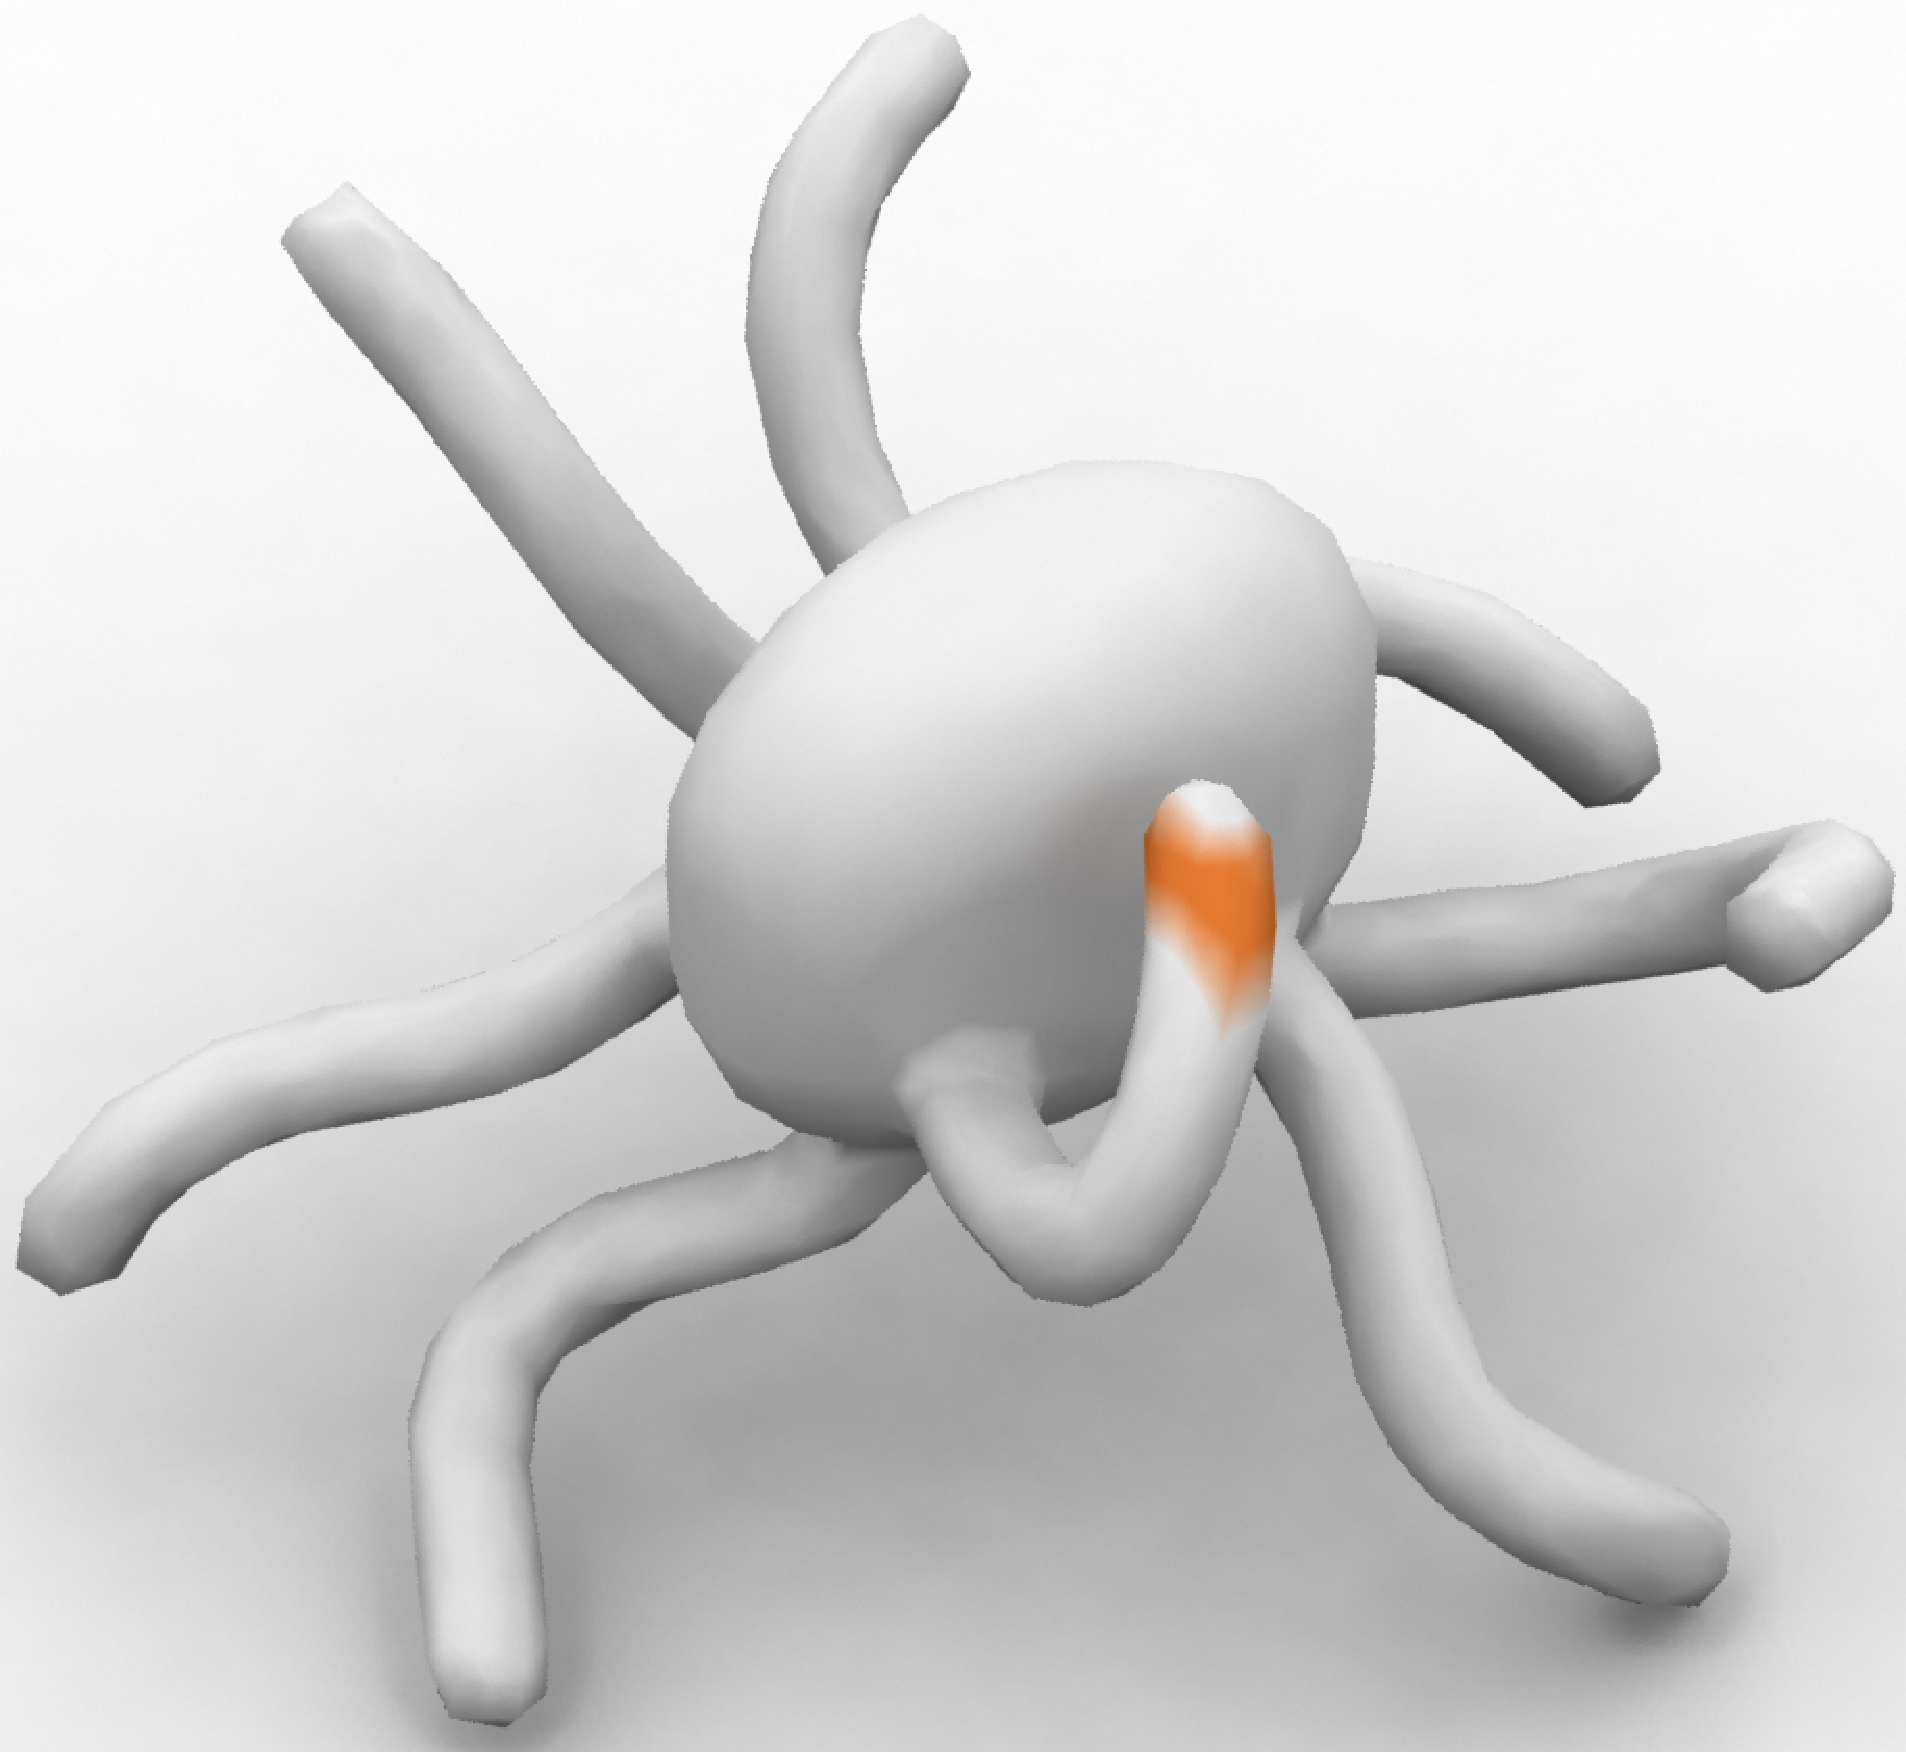
\includegraphics[height=.16\linewidth]{figures/regularization/target_octopus1_0.0007.pdf}
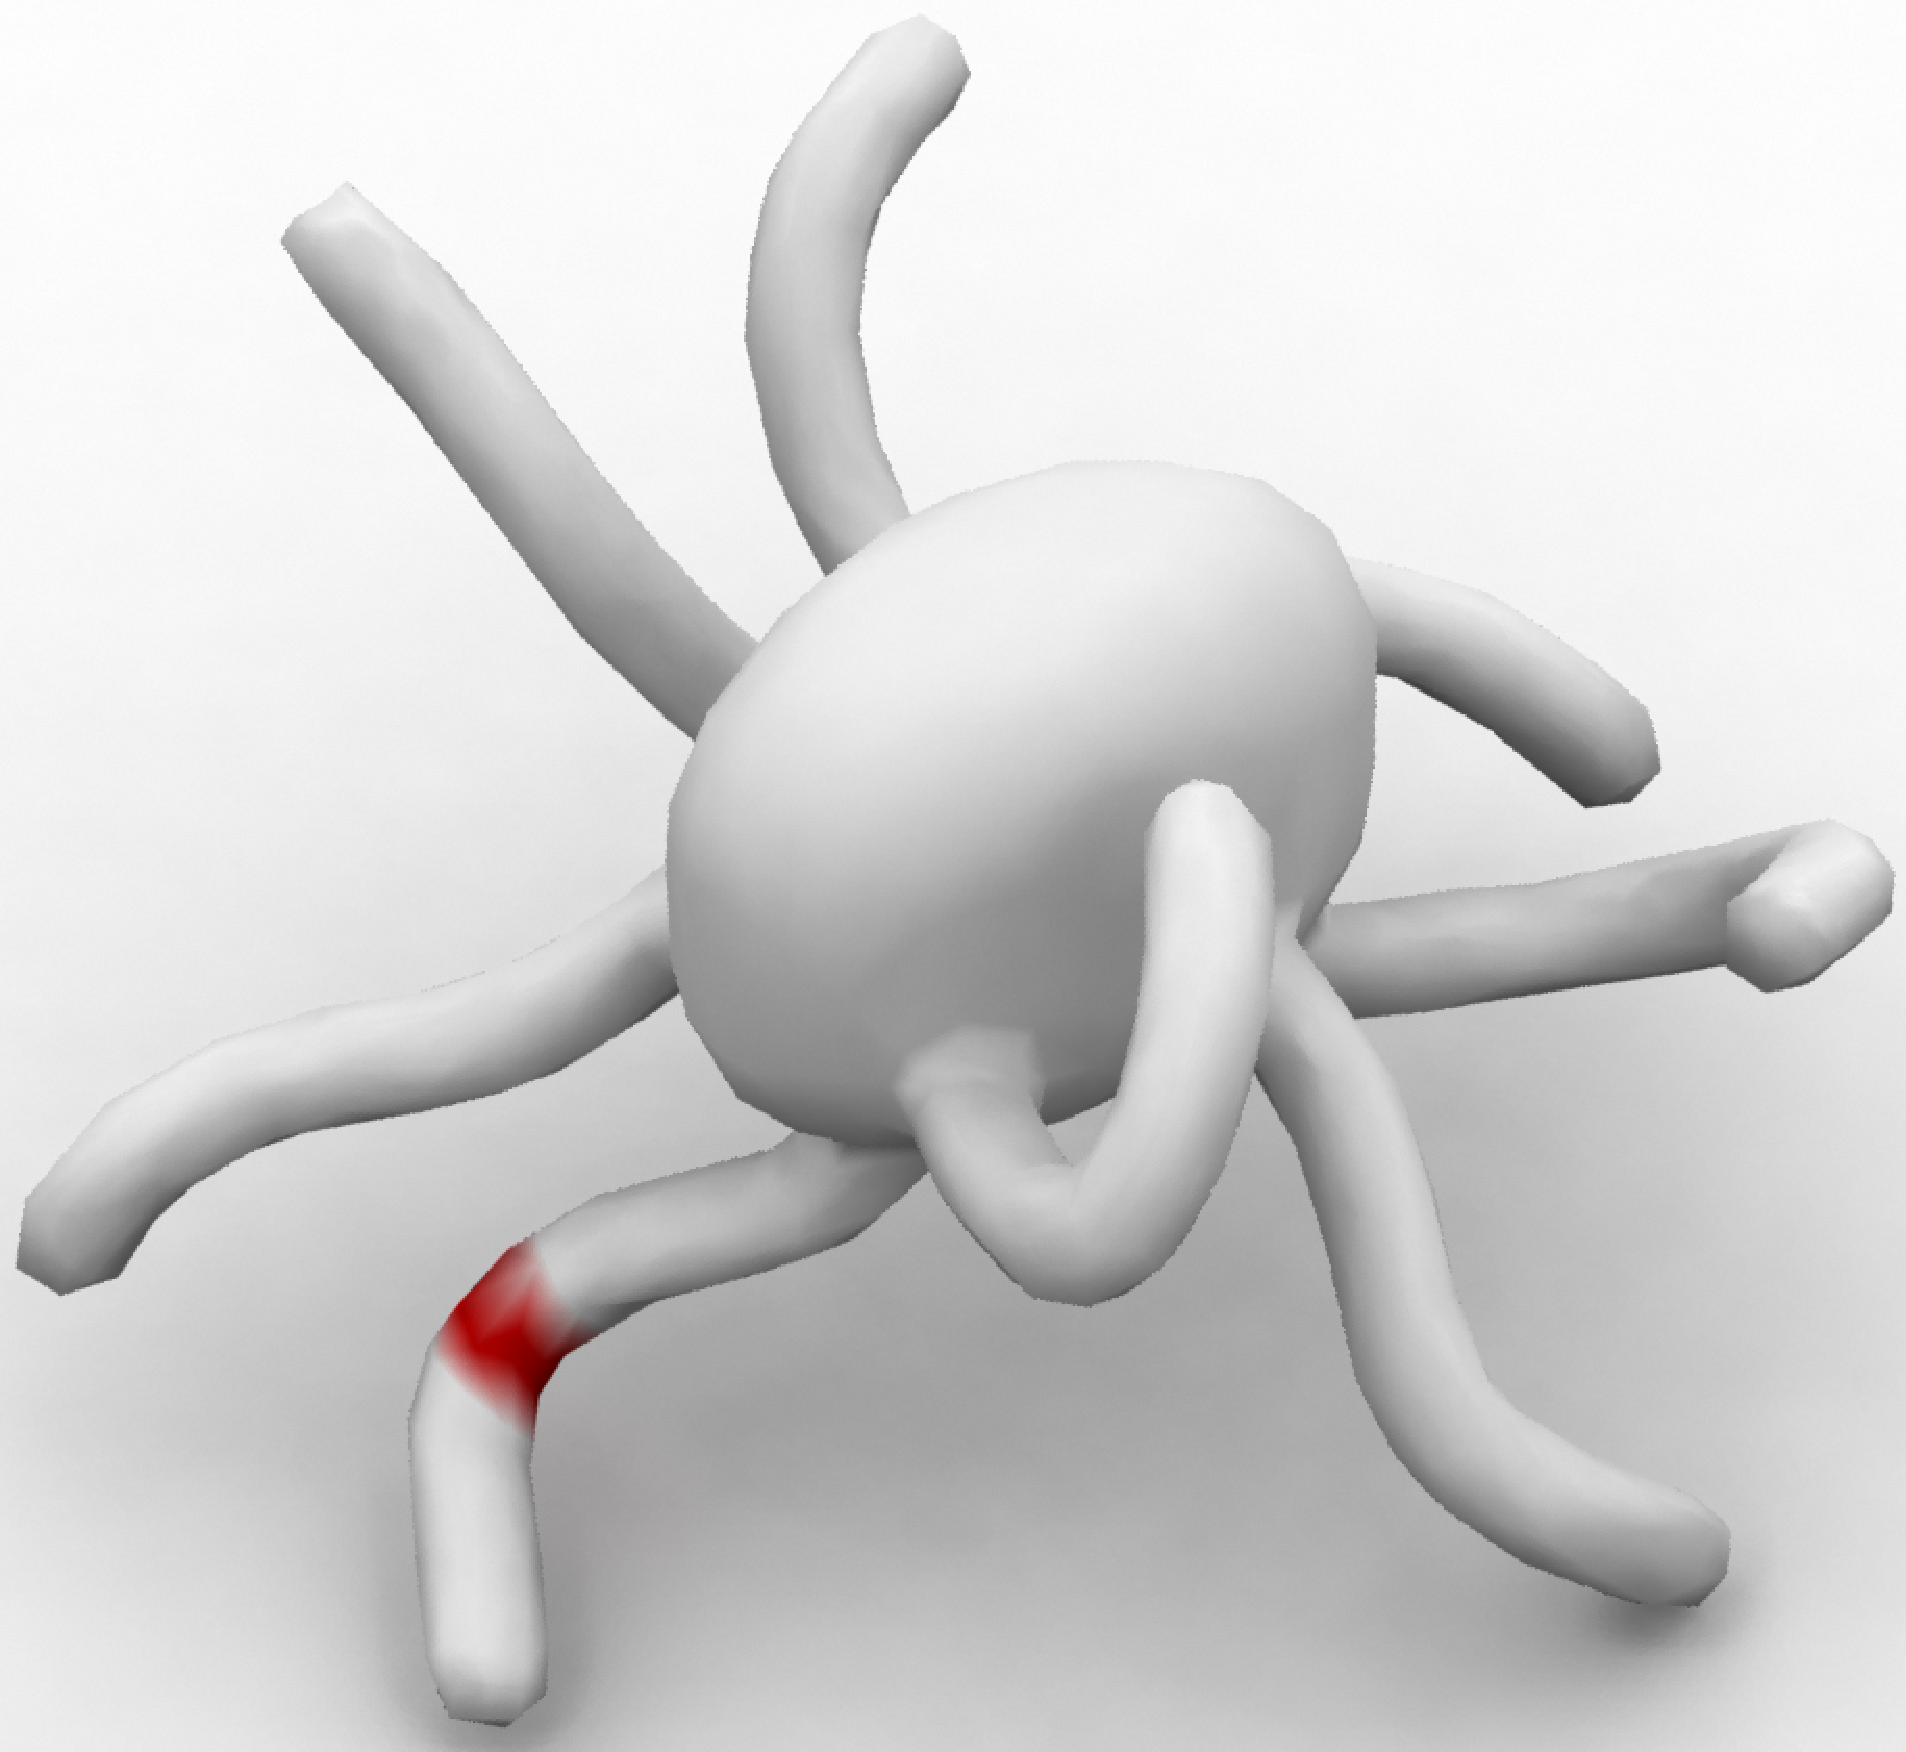
\includegraphics[height=.16\linewidth]{figures/regularization/target_octopus2_0.0007.pdf}
\\
Source surface
& Target surface ($\alpha=8\times10^{-3}$)
& Target surface ($\alpha=7\times10^{-4}$)
\end{tabular}
\caption{Effect of regularization parameter $\alpha$.  Colored points (left) are mapped to colored distributions (right).  As $\alpha$ decreases, the map sharpens; eventually, eight-way symmetry is broken in favor of a more bijective map matching tentacles based on asymmetries in their lengths.\vspace{-.2in}}\label{fig:reg}
\end{figure*}
Suppose we regularize the objective~\eqref{eq:discrete_optim_noreg} by adding $-\alpha H(\G)$ for some  $\alpha>0$.  As illustrated in Figure~\ref{fig:reg}, larger values of $\alpha$ increase the softness of $\G$, effectively smoothing the base GW objective function.  As $\alpha\rightarrow0$, optimal matchings $\G$ begin to resemble permutation matrices (see~\cite[eq.\ (10)]{quadrianto-2009}) and no longer superpose symmetric matches.

Now, define the \emph{KL-divergence} between $\G,\overline{\G}\in\R^{n_0\times n}_+$ as
$$\KL(\G|\overline{\G})\eqdef\sum_{ik} \bmu_{0i}\bmu_k \left[\left(\G\!_{ik} \ln\frac{\G\!_{ik}}{\overline{\G}\!_{ik}}\right)-\G\!_{ik}+\overline{\G}\!_{ik}\right]\!.$$
%\suv{Is the subsequent sentence needed? This particular KL divergence is also called the I-Divergence or simply generalized KL as you note.}%can't hurt to leave it there, right
This KL divergence contains an additional linear term from the one in~\cite{solomon-2015}, but since it only involves $\overline{\G}$ it is a constant in their objective.  This use of ``generalized'' KL (also called $I$-divergence) will figure into our method for joint domain analysis (\S\ref{sec:consistency}) and identifies KL divergence as a Bregman divergence~\cite{bregman-1967}.

\begin{algorithm}[t]
\fbox{\hspace{-.1in}\parbox{\columnwidth}{%
\begin{algorithmic}
\Function{Gromov-Wasserstein}{$\bmu_0,\D_0,\bmu,\D,\alpha,\eta$}
	\LineComment{Computes a local minimizer $\G$ of~\eqref{eq:reg_gw}}
	\algspace
	\Let{$\G$}{\Call{Ones}{$n_0\times n$}}
	\For{$i=1,2,3,\ldots$}
		\Let{$\K$}{$\exp(\D_0\diag{\bmu_0}\G\diag{\bmu}\D^\top/\alpha)$}
		\Let{$\G$}{\Call{Sinkhorn-Projection}{$\K^{\wedge \eta}\otimes \G^{\wedge (1-\eta)};\bmu_0,\bmu$}}
	\EndFor
%	\algspace
	\State\Return{$\G$}
\EndFunction
  \end{algorithmic}
}}
\algspace\\
\fbox{\hspace{-.1in}\parbox{\columnwidth}{%
\begin{algorithmic}
\Function{Sinkhorn-Projection}{$\K;\bmu_0,\bmu$}
	\LineComment{Finds $\G$ minimizing $\KL(\G|\K)$ subject to $\G\in\bM(\bmu_0,\bmu)$}
	\algspace
	\Let{$\v,\w$}{$\1$}%\Comment{Maintains $\G=\diag{\v}\G'\diag{\w}$}
	\For{$j= 1,2,3,\ldots$}
		\Let{$\v$}{$\1 \oslash \K(\w\otimes\bmu)$}
		\Let{$\w$}{$\1 \oslash \K^\top (\v\otimes\bmu_0)$}
	\EndFor
%	\algspace
	\State\Return{$\diag{\v}\K\diag{\w}$}
\EndFunction
  \end{algorithmic}
}}
\vspace{-3mm}
\caption{Iteration for finding regularized Gromov-Wasserstein distances.  $\otimes,\oslash$ denote elementwise multiplication and division.\vspace{-.2in}}\label{alg:gw}
\end{algorithm}

Finally, define
$$\f_\alpha(\G)\eqdef \exp(\D_0\diag{\bmu_0}\G\diag{\bmu}\D/\alpha).$$
After regularizing by adding $-\alpha H(\G)$ to the objective~\eqref{eq:discrete_optim_noreg}, an identical argument to the one in~\cite{benamou-2015} shows that we can recover $\G$ by solving the following minimization problem: % The resulting regularized version of~\eqref{eq:discrete_optim_noreg} can be written as
\begin{equation}\label{eq:reg_gw}
%\bGWa(\D_0,\D)\eqdef
\argmin_{\G\in\bM(\bmu_0,\bmu)} \alpha\KL(\G|\f_\alpha(\G)).
\end{equation}
The fact that $\G$ appears twice makes this objective nonconvex.  As derived in Appendix~\ref{appendix:convergence}, we compute $\G$ using KL-projected gradient descent:%\gabriel{maybe some more details would be welcome, it might not be obvious to everyone why this is a projected gradient. }
%\suv{What does gradient descent in the KL metric really mean? KL is no metric...}%changed to "kl-projected gradient descent"
\begin{equation}\label{eq:fixed_point_gw}
\boxed{\G^{(k\!+\!1)}\!\gets\!\argmin_{\G\in\bM}%(\bmu_0,\bmu)}
%
\KL\!\left(\!\G\!
\left|\!
\left[\f_\alpha(\G^{(k)})\right]^{\wedge\eta}\!\otimes\!\left[\G^{(k)}\right]^{\wedge(1-\eta)}\right.
\!\right)\!,}
\end{equation}
where $\otimes$ denotes elementwise (Hadamard) matrix multiplication.

Iteration~\eqref{eq:fixed_point_gw} is a convex program identical to the optimal transportation problems considered in~\cite{benamou-2015}; as derived in that paper, it can be optimized using iterative Sinkhorn projection.  The parameter $\eta\in(0,1]$ controls the \emph{inertia} of the iterative scheme; $\eta$ acts similarly to the ``learning rate'' parameter of gradient descent algorithms.  Pseudocode is provided in Algorithm~\ref{alg:gw}.  

\subsection{Convergence}\label{sec:convergence}

Convergence of~\eqref{eq:fixed_point_gw} as $k\rightarrow\infty$ is a subtle matter.  While existing work suggests monotonicity of the objective~\eqref{eq:reg_gw} under weak assumptions (see below), this does \emph{not} guarantee convergence of the iterates $\G^{(k)}\!$.  Given the dependence of our subsequent discussion on this algorithm as well as its appearance in many other contexts, we prove the following convergence result:
\begin{proposition}\label{prop:gw_convergence}
$\{\G^{(k)}\}_{k=0}^\infty$ converges to a critical point of~\eqref{eq:reg_gw} when $\eta<\nicefrac{c\alpha}{1+c\alpha}$, where $c\eqdef[\min_{ij}\bmu_{0i}\bmu_j]/\|\bmu_0\|^2\|\bmu\|^2\|\D_0\|\|\D\|$.
\end{proposition}
As $\alpha$ increases, the required bound loosens, reflecting the improved conditioning of the optimization problem.  We prove this result in the appendix by expressing it as an instance of a modern method for nonconvex optimization~\cite{bot-2015}.

From a practical standpoint, we halt \GWa iteration when the relative change in $\G$ or objective value is less than a fixed threshold ($10^{-7}$ in our experiments).

\paragraph*{Comparison to softassign.}  While we derived it for \GWa matching, iteration~\eqref{eq:fixed_point_gw} with $\eta=1$ is similar to the ``softassign'' algorithm in machine learning for quadratic assignment~\cite{gold-1996,rangarajan-1996}.  %, although this work only considers convex instances of the non-regularized quadratic correspondence problem and hence cannot deal with symmetric matching.
Rangarajan et al.~\shortcite{rangarajan-1997,rangarajan-1999} consider the convergence of softassign.  They mainly focus on monotonicity of the objective rather than convergence of the iterates.  More critically, their analysis assumes convexity; see, e.g., the conclusion of the proof of~\cite[Theorem 1]{rangarajan-1999}.  Such an assumption is unlikely to be valid for geometric problems with local and global symmetries.  Their analysis introduces convexity via a ``self-amplification term'' along the diagonal of the objective matrix, which modifies the optimization problem and obliterates the possibility of identifying symmetric ambiguity.

\subsection{Parameter Selection}

%\vova{Can we somehow guess an appropriate level of regularization?  Vova suggests showing that you can get away with low regularization when the shapes are isometric, and more is needed as you deviate from isometry.}

\begin{figure}\centering\pgfplotsset{scaled y ticks=false}
\begin{tikzpicture}
\begin{axis}[xlabel={\footnotesize $\alpha$},ylabel={\footnotesize Objective term},width=\columnwidth,height=.5\columnwidth,
xlabel near ticks,
ylabel near ticks,
line cap = round,
line join = round,
xlabel shift = -.04in,
ylabel shift = -.08in,
xmin = 0.0007,
xmax = .1,
ymin = 0,
yticklabel style={
        /pgf/number format/fixed,
        /pgf/number format/precision=3
},xmode=log,%ymode=log,
scaled y ticks=false,legend cell align=left]%,legend pos = south west]
\addplot[mark=none,color=blue,thick] table[x index=0,y index=1,col sep=comma,mark=none] {figures/alpha/alphatest.txt};\addlegendentry{\footnotesize $\langle \G,\bL(\G)\rangle$};
\addplot[mark=none,color=purple,thick] table[x index=0,y index=2,col sep=comma,mark=none] {figures/alpha/alphatest.txt};\addlegendentry{\footnotesize $-H(\G)$};
\end{axis}
\end{tikzpicture}
\vspace{-.15in}
\caption{Dependence of objective terms on regularizer $\alpha$ for the experiment in Figure~\protect\ref{fig:reg}.\vspace{-.15in}}\label{fig:regularizer}
\end{figure}

%\gabriel{So the conclusion here seems to be that large $\alpha$ is not so helpful :( This somehow contradict the conclusion of the article, I found.}\justin{how so?  large alpha makes for fast convergence and maps that superpose symmetries, both good things for fuzzy mapping!  added a few sentences}

Figure~\ref{fig:regularizer} illustrates the trade-off between the two objective terms for the experiments in Figure~\ref{fig:reg} as a function of $\alpha$.  As $\alpha$ increases, so does the GW objective~\eqref{eq:GW2} while negative entropy decreases.  A phase transition in the GW objective indicates a change in the nature of the map, in this case from mapping individual tentacles to superposing all tentacle targets.  This example illustrates a more general pattern:  large choices of $\alpha$ lead to higher-entropy correspondence matrices that still contain meaningful match information, while lower $\alpha$'s make for sharper map matrices that express a single coherent matching.  When $\alpha$ is small but there exist multiple symmetric maps, they can be extracted using the method in \S\ref{sec:symmetry}.

Our algorithm converges faster with a warm start, and hence we can generate plots like the one in Figure~\ref{fig:regularizer} efficiently by incrementally adjusting $\alpha$ and updating $\G$.  User-guided selection of $\alpha$ can be guided using this plot to find significant changes in the map as it depends on regularization.



% Doesn't seem to work
%\section{Partial Matching}
%
%If we assume that every point in $\source$ has some match in $\target$ but not necessarily the reverse, then we should not optimize in the space of measure couplings $\M(\mu_0,\mu)$ but rather in a simpler space of measures satisfying only the first constraint $\gamma(S_0\times \target)=\mu_0(S_0)\,\forall S_0\subseteq\source.$
%
%Discretely, this suggests a larger space of partial couplings:
%$$\bP(\bmu_0,\bmu)\eqdef\{\G\in\R_+^{n_0\times n} : \G\bmu=\1\}.$$
%Iterative optimization of our regularized objective with this new set of constraints is essentially the same as before~\eqref{eq:fixed_point_gw}:
%\begin{equation}
%\boxed{
%\G^{(k\!+\!1)}\!\gets\!
%\argmin_{\G\in\bP}\!\,\KL\!\left(
%\!\G\!\left|\!\,
%\exp\!\left(-\frac{\eta}{\alpha}\bL(\G^{(\!k\!)})\!\right)
%\!\otimes\!
%\left[\!\G^{(\!k\!)}\!\right]\!^{\!\wedge\!(1\!-\!\eta)}
%\right.
%\right)\!
%}
%\end{equation}
%In this case, the KL projection is even simpler than the Sinkhorn projection needed in \S\ref{sec:entropic_reg}; rather than requiring iterative normalization, the rows of the kernel are simply scaled to integrate to one.
%
%Taking the partial matching philosophy to the extreme, we could remove all marginal constraints on $\G$ and instead require that it represent a general distribution over $\source\times\target$.   In discrete language, this variation corresponds to constraining only $\bmu_0^\top\G\bmu=1$ and $\G\geq0$.  KL projection onto this set maps $\K\mapsto\K/(\bmu_0^\top\K\bmu)$. 
%
% This final relaxation is dangerous in the continuous case and even discretely when the entropic regularizer is not introduced.  In the extreme, $\G$ could have just a single nonzero entry matching a single point on the source and target.  The entropic regularizer, however, counteracts this concentrated match by encouraging $\G$ to have a wider distribution of nonzero entries.  Both algorithms for partial matching are made explicit in Algorithm~\ref{alg:partial_gw}.
%
%
%\begin{algorithm}[t]
%\fbox{\hspace{-.1in}\parbox{\columnwidth}{%
%\begin{algorithmic}
%\Function{Partial-Source-GW}{$\bmu_0,\D_0,\bmu,\D,\alpha$}
%	\LineComment{Gromov-Wasserstein with only prescribed row sums}
%	\algspace
%	\Let{$\G$}{\Call{Ones}{$n_0\times n$}}
%	\For{$i=1,2,3,\ldots$}
%		\Let{$\K$}{
%$
%\left\{
%\begin{array}{r@{}l}
%\exp[\frac{1}{\alpha}
%(\D_0&\diag{\bmu_0}\G\diag{\bmu}\D^\top\\
%&-\frac{1}{2}\1\bmu_0^\top\G\diag{\bmu}\D^{\wedge2})]
%\end{array}\right.
%$}
%		\Let{$\K$}{$\K^{\wedge \eta}\otimes\G^{\wedge(1-\eta)}$}
%		\Let{$\G$}{$\K\oslash (\K\bmu\1^\top)$}
%	\EndFor
%	\algspace
%	\State\Return{$\G$}
%\EndFunction
%  \end{algorithmic}
%}}
%\algspace\\
%\fbox{\hspace{-.1in}\parbox{\columnwidth}{%
%\begin{algorithmic}
%\Function{Partial-to-Partial-GW}{$\bmu_0,\D_0,\bmu,\D,\alpha$}
%	\LineComment{Gromov-Wasserstein without prescribed marginals}
%	\algspace
%	\Let{$\G$}{\Call{Ones}{$n_0\times n$}}
%	\For{$i=1,2,3,\ldots$}
%		\Let{$\K$}{
%$
%\left\{
%\begin{array}{r@{}l}
%\exp[\frac{1}{\alpha}
%(\D_0&\diag{\bmu_0}\G\diag{\bmu}\D^\top\\
%&-\frac{1}{2}\1\bmu_0^\top\G\diag{\bmu}\D^{\wedge2}\\
%&-\frac{1}{2}\D_0^{\wedge2}\diag{\bmu_0}\G\bmu\1^\top
%)]
%\end{array}\right.
%$}
%		\Let{$\K$}{$\K^{\wedge \eta}\otimes\G^{\wedge(1-\eta)}$}
%		\Let{$\G$}{$\K/(\bmu_0^\top \K\bmu)$}
%	\EndFor
%	\algspace
%	\State\Return{$\G$}
%\EndFunction
%  \end{algorithmic}
%}}
%\caption{Algorithms for partial matching that optimize the Gromov-Wasserstein objective.}\label{alg:partial_gw}
%\end{algorithm}


%%% Local Variables:
%%% mode: latex
%%% TeX-master: "../gw"
%%% End:

% !TEX root = ../gw.tex

%\suv{Hopefully after my comments are gone, the figures show up in correct sequence!}
\section{Experiments}\label{sec:experiments}

Algorithm~\ref{alg:gw} provides an extremely simple technique for optimizing the \GWa objective function.  We view this simplicity as an advantage; our algorithm is implementable in nearly any framework and generalizable to many classes of domains.  In this section, we verify that simplicity does not come at the cost of performance through experiments designed to reveal properties of our iterative technique.

\paragraph*{Convergence.}

\begin{figure}[t]\centering\pgfplotsset{scaled y ticks=false}
\begin{tikzpicture}
\begin{axis}[xlabel={\footnotesize Iteration},ylabel={\footnotesize \GWa objective},width=\columnwidth,height=.6\columnwidth,xlabel near ticks,ylabel near ticks,line cap = round,
line join = round,
xlabel shift = -.08in,
ylabel shift = -.08in,
xmin = 1,
xmax = 50,
yticklabel style={
        /pgf/number format/fixed,
        /pgf/number format/precision=3
},
scaled y ticks=false,legend cell align=left]
\addplot[mark=none,color=lightgray,thick,dotted] table[x index=0,y index=6,col sep=comma,mark=none,color=lightgray] {figures/eta/data_0.008.txt};\addlegendentry{\footnotesize $\eta=2$};
\addplot[mark=none,color=cyan,thick] table[x index=0,y index=5,col sep=comma,mark=none] {figures/eta/data_0.008.txt};\addlegendentry{\footnotesize $\eta=1$};
\addplot[mark=none,color=purple,thick] table[x index=0,y index=4,col sep=comma,mark=none] {figures/eta/data_0.008.txt};\addlegendentry{\footnotesize $\eta=2^{-1}$};
\addplot[mark=none,color=blue,thick] table[x index=0,y index=3,col sep=comma,mark=none] {figures/eta/data_0.008.txt};\addlegendentry{\footnotesize $\eta=2^{-2}$};
\addplot[mark=none,color=green,thick] table[x index=0,y index=2,col sep=comma,mark=none] {figures/eta/data_0.008.txt};\addlegendentry{\footnotesize $\eta=2^{-3}$};
\addplot[mark=none,color=red,thick] table[x index=0,y index=1,col sep=comma,mark=none] {figures/eta/data_0.008.txt};\addlegendentry{\footnotesize $\eta=2^{-4}$};
\end{axis}
\end{tikzpicture}\\\vspace{-.05in}
(a) $\alpha=8\times10^{-3}$\\\vspace{.05in}
%
%
\begin{tikzpicture}
\begin{axis}[xlabel={\footnotesize Iteration},ylabel={\footnotesize \GWa objective},width=\columnwidth,height=.6\columnwidth,xlabel near ticks,ylabel near ticks,line cap = round,
line join = round,
xlabel shift = -.08in,
ylabel shift = -.08in,
xmin = 1,
xmax = 50,
yticklabel style={
        /pgf/number format/fixed,
        /pgf/number format/precision=3
},
scaled y ticks=false,legend cell align=left]
\addplot[mark=none,color=cyan,thick] table[x index=0,y index=5,col sep=comma,mark=none] {figures/eta/data_0.0007.txt};\addlegendentry{\footnotesize $\eta=1$};
\addplot[mark=none,color=purple,thick] table[x index=0,y index=4,col sep=comma,mark=none] {figures/eta/data_0.0007.txt};\addlegendentry{\footnotesize $\eta=2^{-1}$};
\addplot[mark=none,color=blue,thick] table[x index=0,y index=3,col sep=comma,mark=none] {figures/eta/data_0.0007.txt};\addlegendentry{\footnotesize $\eta=2^{-2}$};
\addplot[mark=none,color=green,thick] table[x index=0,y index=2,col sep=comma,mark=none] {figures/eta/data_0.0007.txt};\addlegendentry{\footnotesize $\eta=2^{-3}$};
\addplot[mark=none,color=red,thick] table[x index=0,y index=1,col sep=comma,mark=none] {figures/eta/data_0.0007.txt};\addlegendentry{\footnotesize $\eta=2^{-4}$};
\end{axis}
\end{tikzpicture}\\\vspace{-.05in}
(b) $\alpha=7\times10^{-4}$
\vspace{-.1in}
\caption{Convergence for the examples in Figure~\ref{fig:reg}.\vspace{-.15in}}\label{fig:convergence}
\end{figure}

%\gabriel{Maybe I am misinterpreting the following paragraphe, but it seems to indicate that large $\eta$ helps to avoid local minimum, but the curve seems to indicate otherwise (small $\eta$ leads to better objective values). Can you explain ? }\justin{i removed a misleading "local" in the last sentence -- maybe this helps?}


Figure~\ref{fig:convergence} illustrates convergence of our algorithm on the experiments in Figure~\ref{fig:reg}, with several choices of $\eta$.  The experiments illustrate that the bound on $\eta$ in Proposition~\ref{prop:gw_convergence} is loose, that is, some choices of $\eta\geq\nicefrac{c\alpha}{1+c\alpha}$ still exhibit convergence.  In our experiments, the algorithm appears to converge monotonically even when $\eta=1$.  While we are unable to provide rigorous proof of convergence in this regime, from an engineering standpoint larger $\eta$ values can hasten completion time. Figure~\ref{fig:convergence}a shows an example with $\eta>1$ that does not converge.  As a trade-off, Figure~\ref{fig:convergence}b illustrates that the larger steps can skip past optima with better objective values; in this case, the different local optima correspond to different matchings of the octopus's tentacles.

\paragraph*{Sensitivity.}  

\begin{figure}[t]\centering\pgfplotsset{scaled y ticks=false}
%
%
\begin{tabular}{c@{}c@{}c}
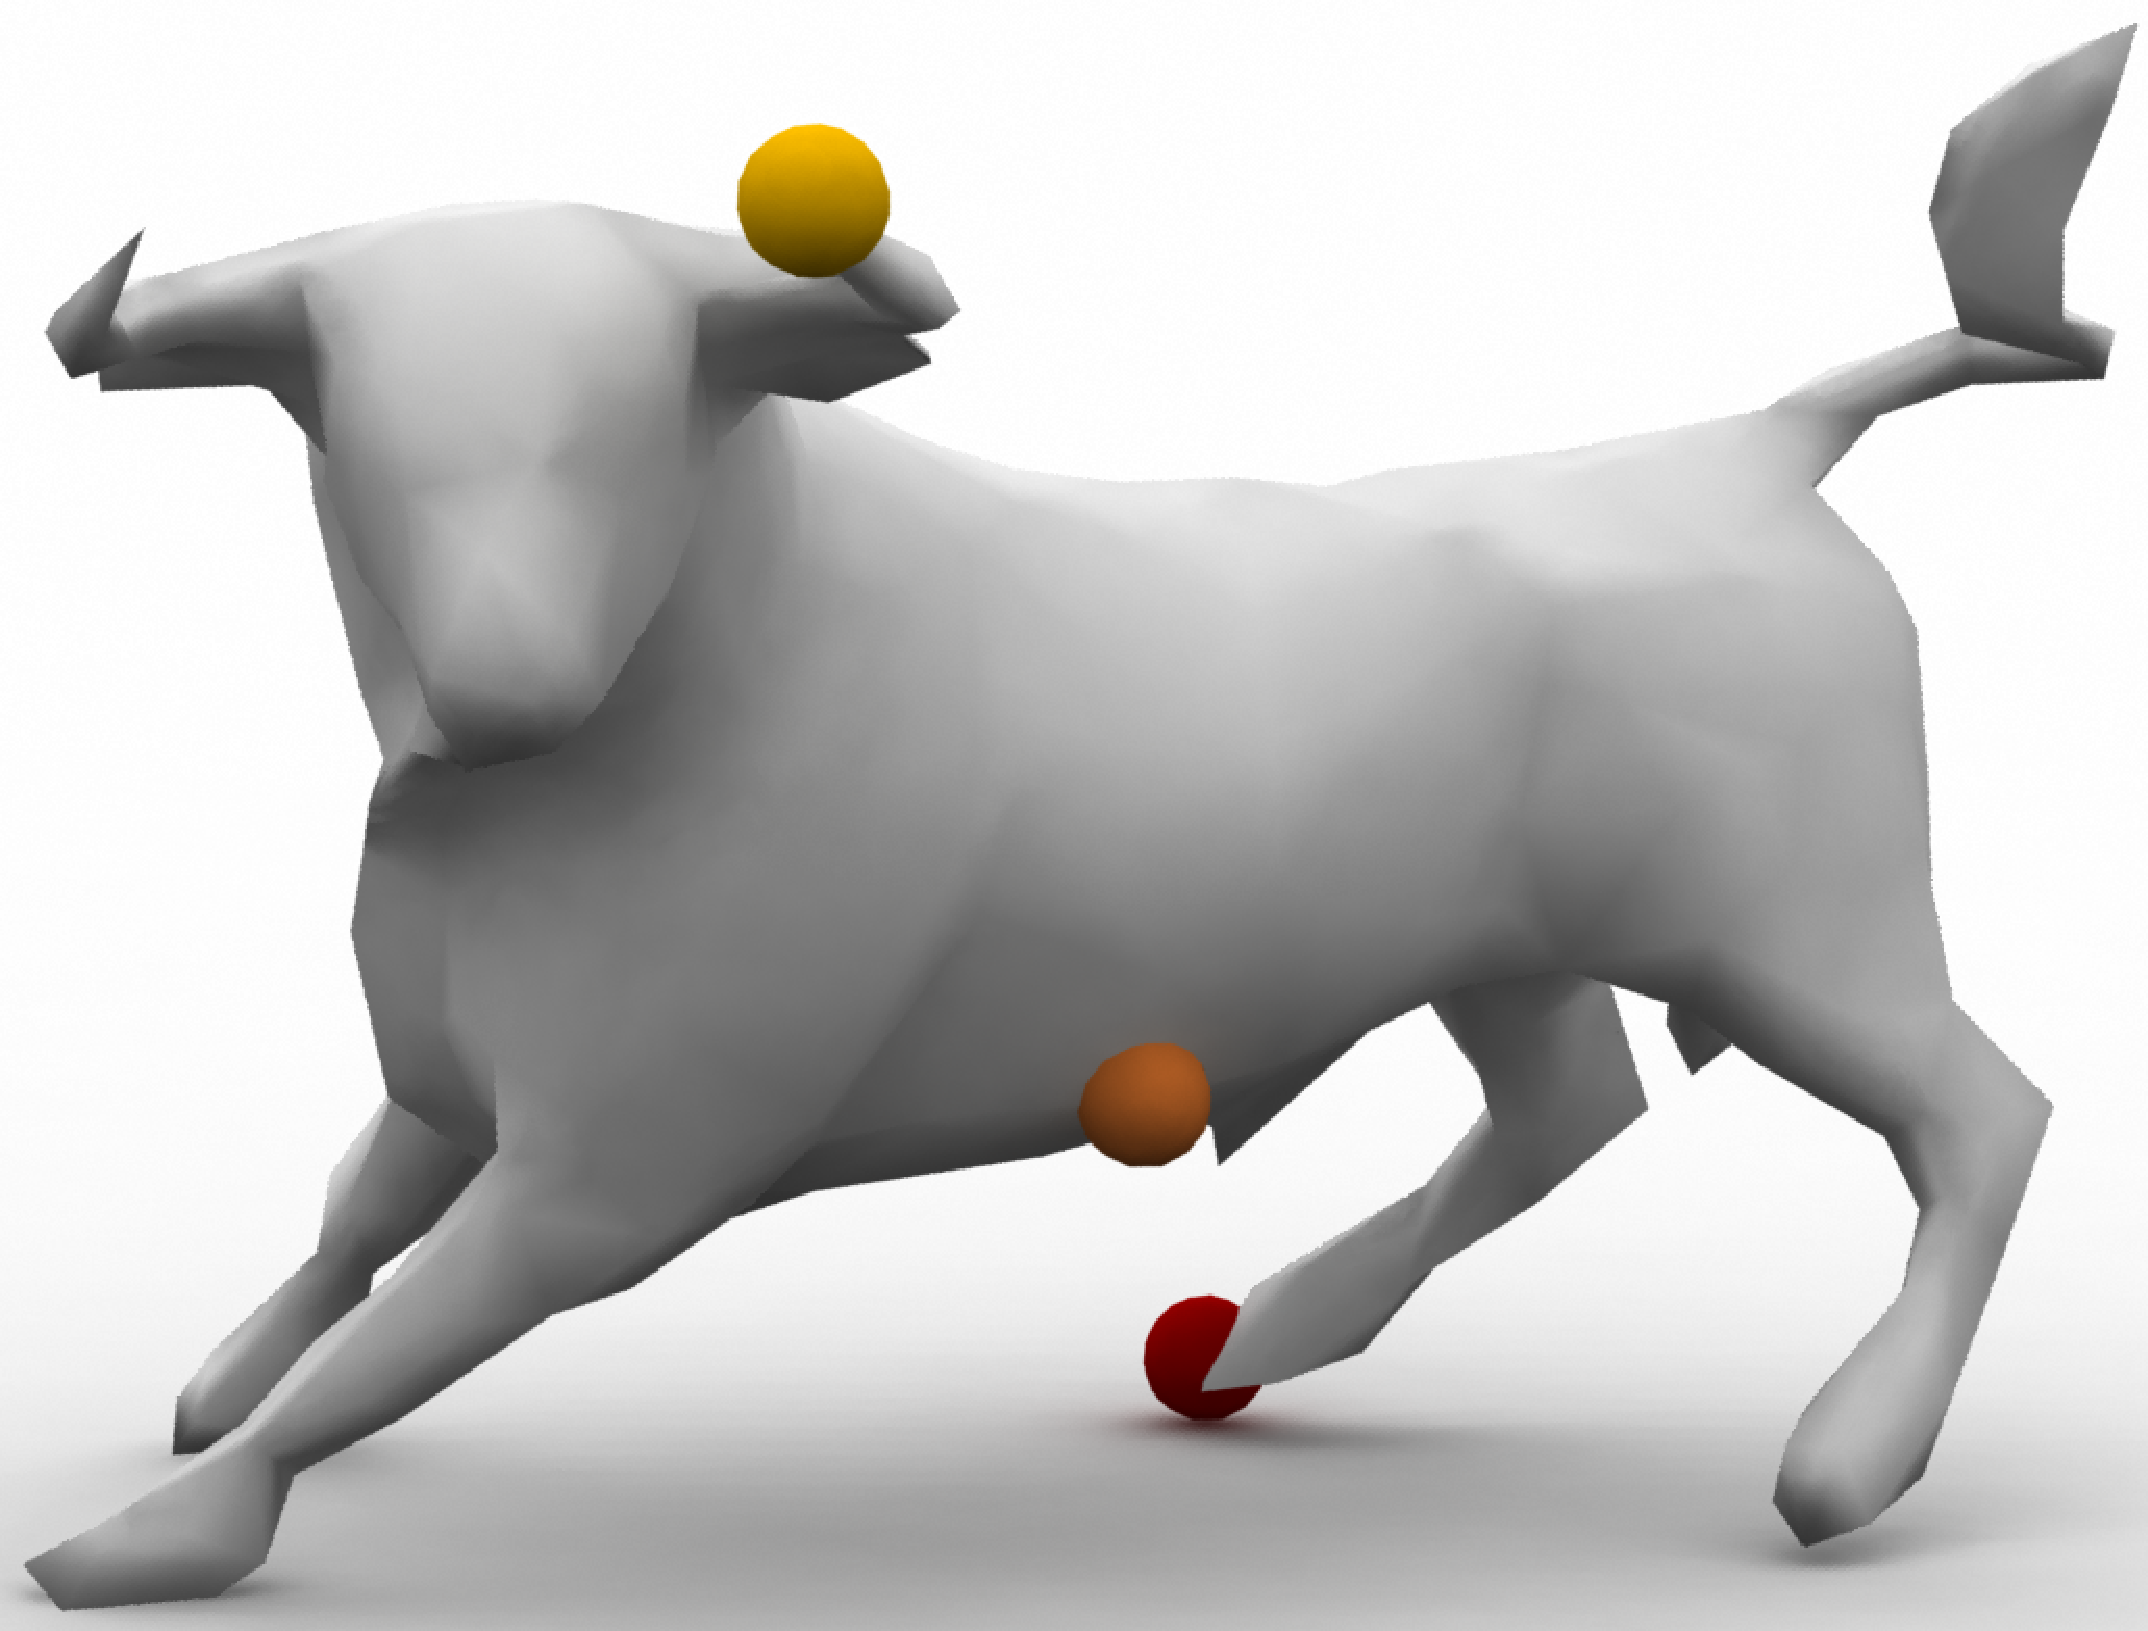
\includegraphics[height=.2\linewidth]{figures/stability/source_bull.pdf}&
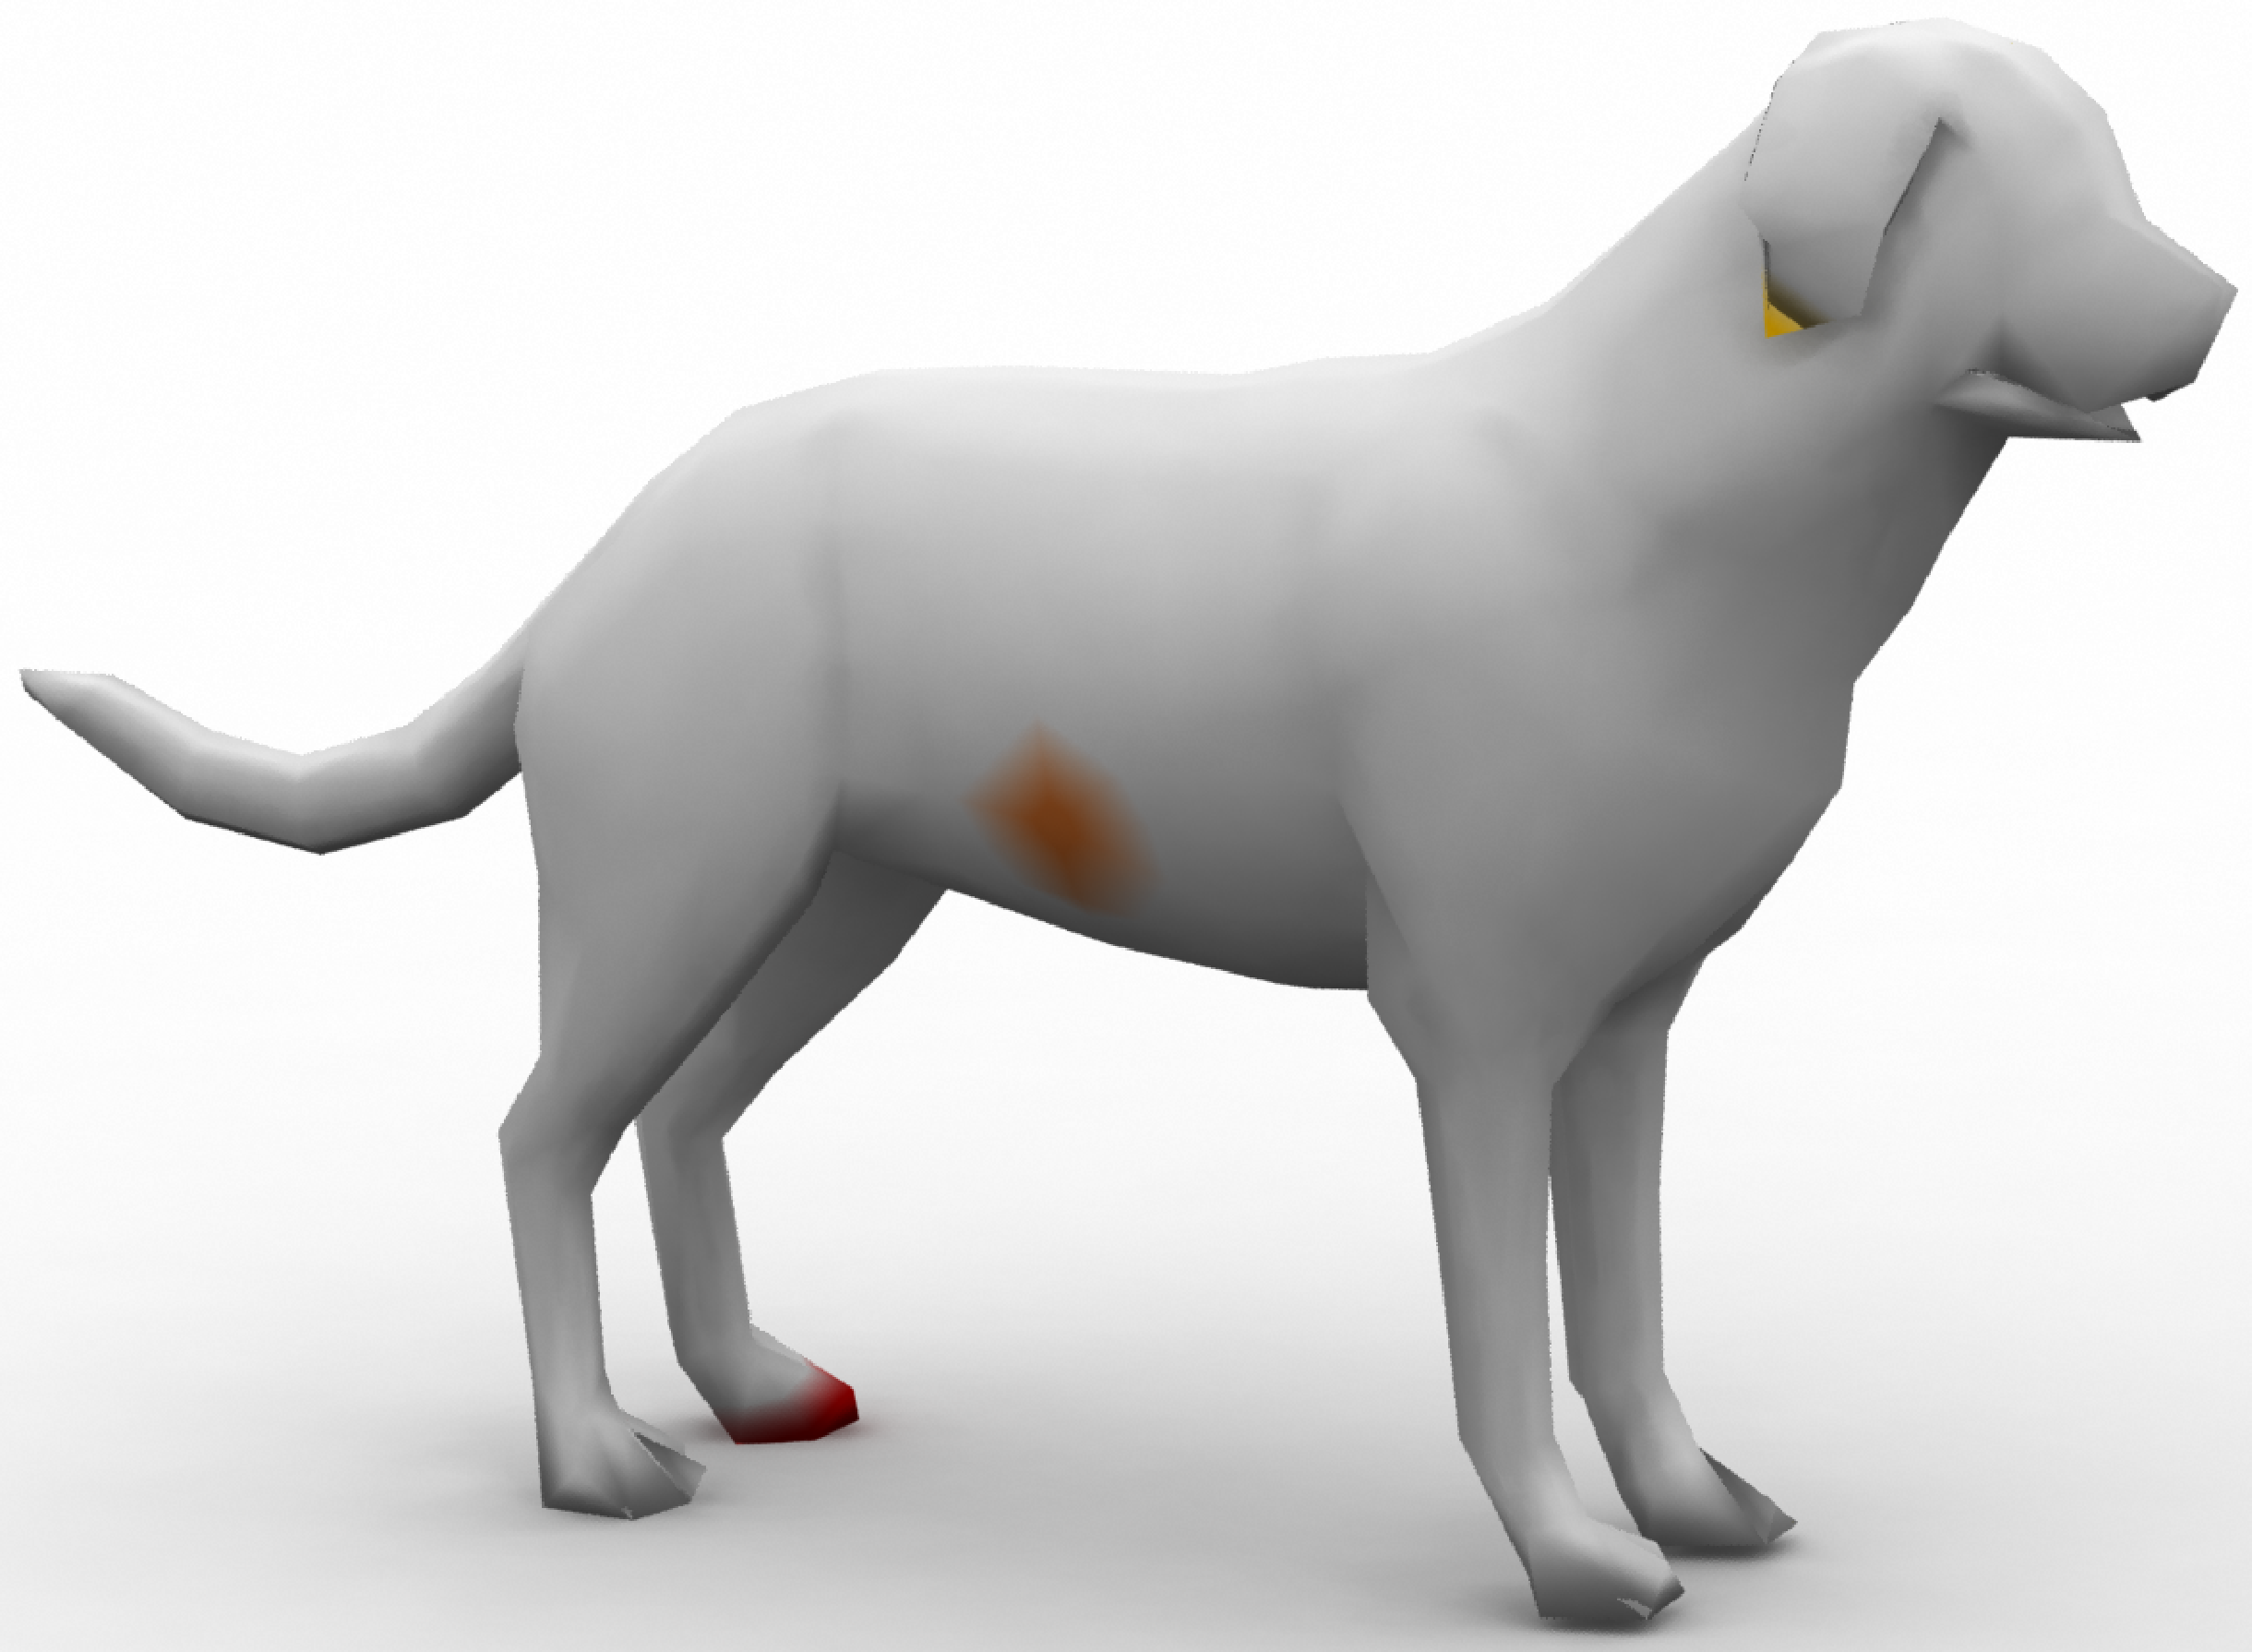
\includegraphics[height=.2\linewidth]{figures/stability/minAlphaTarget_cropped.pdf}&
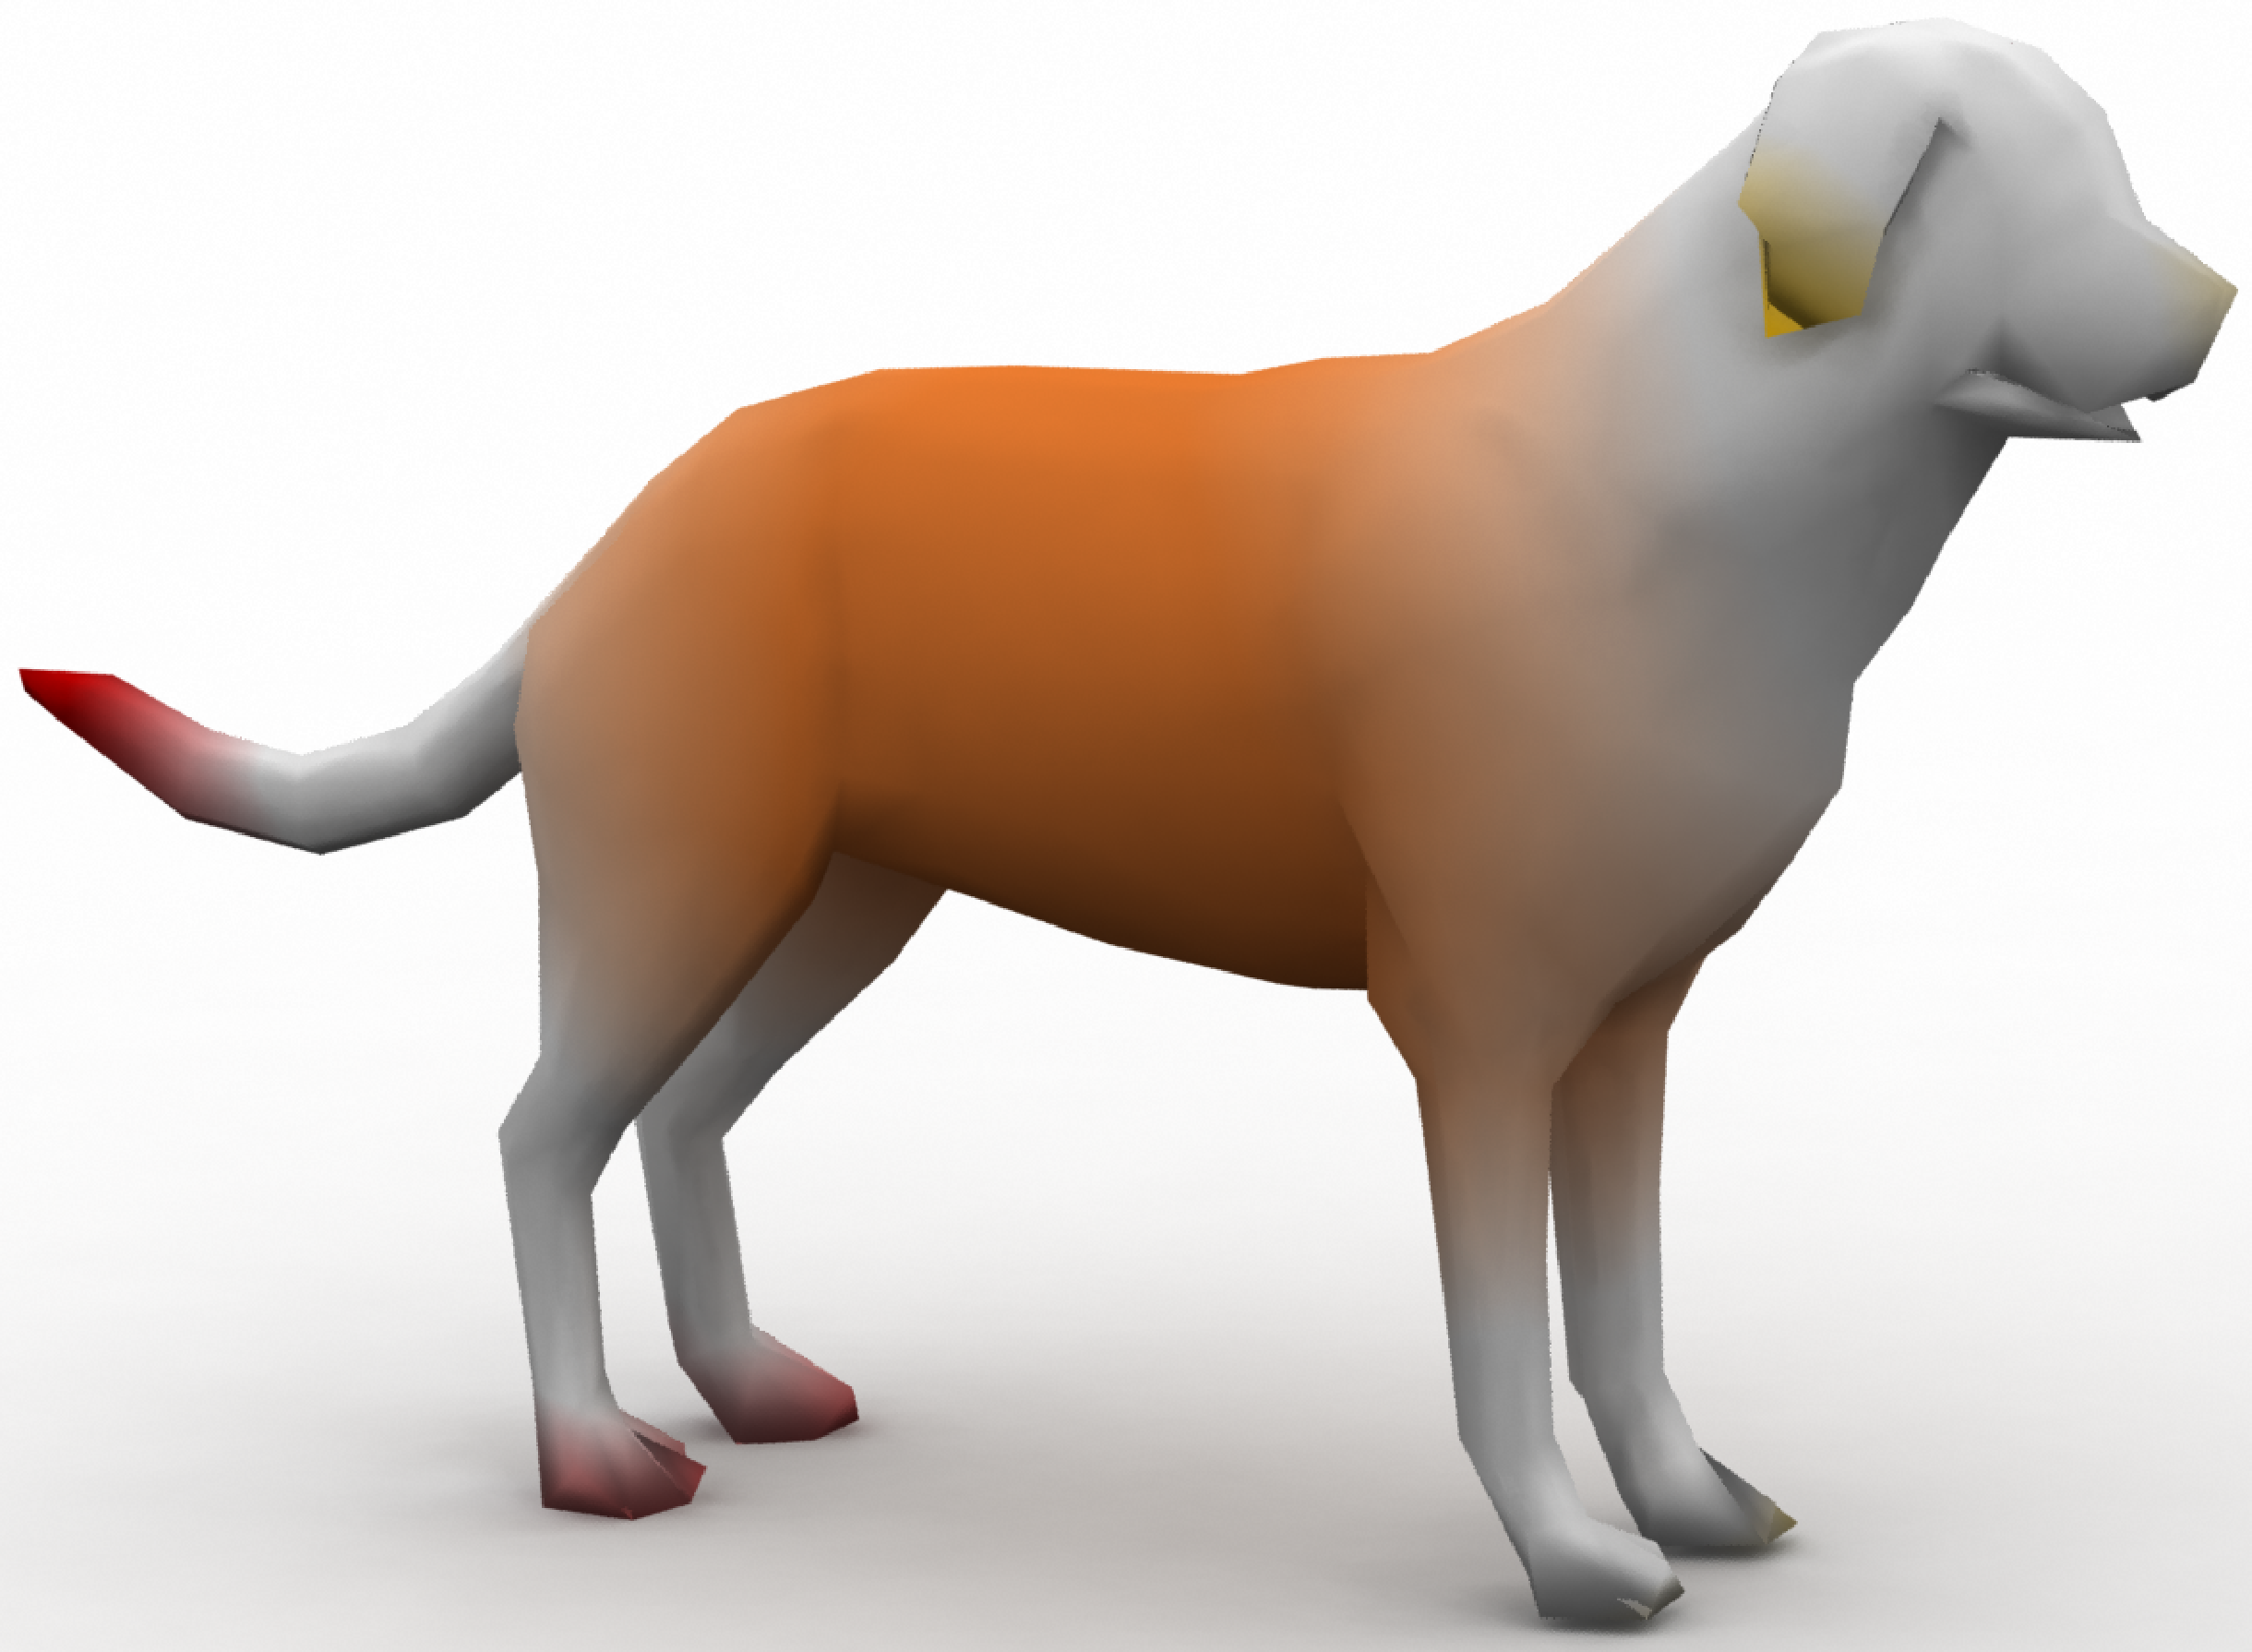
\includegraphics[height=.2\linewidth]{figures/stability/maxAlphaTarget_cropped.pdf}\\
\small Source & \small$\alpha=5\times 10^{-4}$ &\small $\alpha=10^{-2}$
\end{tabular}
%
%
\begin{tikzpicture}
\begin{axis}[xlabel={\footnotesize $\alpha$},ylabel={\footnotesize Objective term},width=\columnwidth,height=.5\columnwidth,
%xlabel near ticks,
ylabel near ticks,
line cap = round,
line join = round,
xlabel shift = -.08in,
ylabel shift = -.08in,
xmin = 0.001,
xmax = .1,
ymin = .2,
yticklabel style={
        /pgf/number format/fixed,
        /pgf/number format/precision=3
},xmode=log,%ymode=log,
scaled y ticks=false,legend cell align=left,legend pos = north west]
\addplot[only marks,color=blue,mark size = .3] table[x index=0,y index=1,col sep=comma,mark=none] {figures/stability/initialGuess.txt};\addlegendentry{\footnotesize $\langle \G,\bL(\G)\rangle$};
\end{axis}
\end{tikzpicture}\\\vspace{-.075in}
(a) Triangle mesh matching ($n_0=n=502$)\\
\vspace{.1in}\hrule
\vspace{.1in}
%
%
\begin{tabular}{cccc}
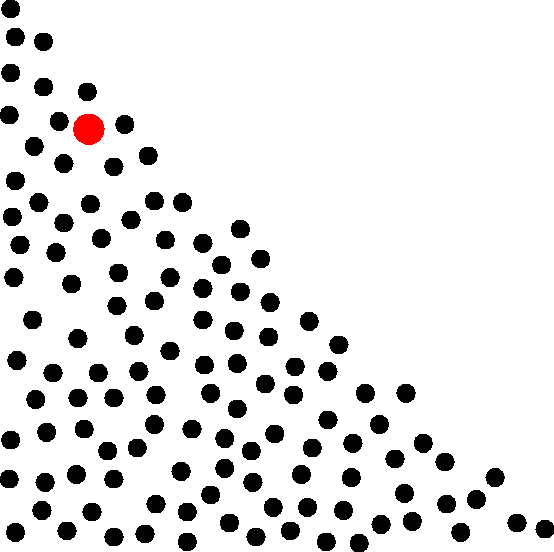
\includegraphics[height=.2\linewidth]{figures/stability/source2d.pdf}&

\includegraphics[height=.2\linewidth]{figures/stability/target2d1.pdf}&

\includegraphics[height=.2\linewidth]{figures/stability/target2d2.pdf}&
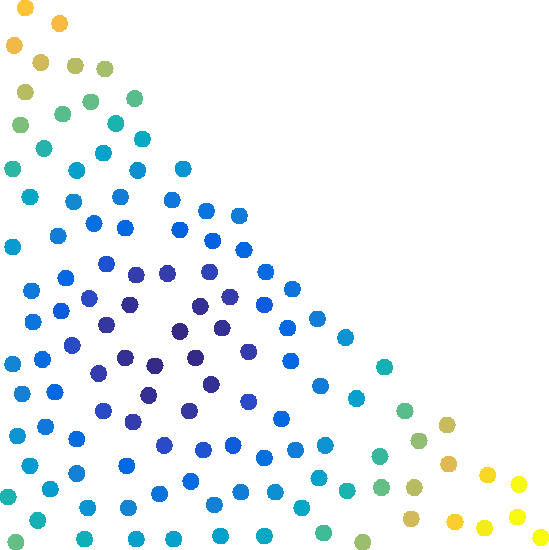
\includegraphics[height=.2\linewidth]{figures/stability/target2d3.pdf}\\
\small Source & \small$\alpha=5\times 10^{-4}$ &\small $\alpha=5\times 10^{-4}$&\small$\alpha=2\times10^{-2}$\vspace{-.05in}\\
& \small\emph{(trial 1)} & \small\emph{(trial 2)}
\end{tabular}\vspace{-.05in}
%
%
\begin{tikzpicture}
\begin{axis}[xlabel={\footnotesize $\alpha$},ylabel={\footnotesize Objective term},width=\columnwidth,height=.5\columnwidth,
%xlabel near ticks,
ylabel near ticks,
line cap = round,
line join = round,
xlabel shift = -.08in,
ylabel shift = -.08in,
xmax = 0.001,
xmin = .0006,
ymin = 0.002,
ymax = .004,
yticklabel style={
        /pgf/number format/fixed,
        /pgf/number format/precision=3
},xmode=log,%ymode=log,
scaled y ticks=false,legend cell align=left,legend pos = north west]
\addplot[only marks,color=blue,mark size = .3] table[x index=0,y index=1,col sep=comma,mark=none] {figures/stability/initialGuess2.txt};\addlegendentry{\footnotesize $\langle \G,\bL(\G)\rangle$};
\end{axis}
\end{tikzpicture}\\\vspace{-.075in}
(b) 2D point sample matching ($n_0=119$, $n=121$)
%
%
\caption{Sensitivity to initial guess of $\G$ for matching (a) surfaces and (b) planar point samples.\vspace{-.2in}}\label{fig:sensitivity}
\end{figure}

Since Algorithm~\ref{alg:gw} optimizes a non-convex objective, the output may depend on the initial $\G$. Figure~\ref{fig:sensitivity} tests sensitivity to the initial guess.  Like the previous test, for a given matching task we plot the optimized GW objective $\langle \G,\bL(\G)\rangle$ as a function of $\alpha$; this roughly should increase as $\alpha$ increases.  In this test, however, we randomly generate an initial $\G$ in each trial.% rather than using the matrix of all ones suggested in Algorithm~\ref{alg:gw}.

We evaluate surface matching stability in Figure~\ref{fig:sensitivity}a; distance matrices $\D_0,\D$ contain geodesic distances.  This test, representative of many similar experiments involving surfaces, shows little dependence on the initial $\G$ even for sharp matchings (low $\alpha$), as reflected by the single coherent curve of objective values.

To reveal a case where multiple optima appear, we consider the task of matching two Poisson disk samples from a right triangle in Figure~\ref{fig:sensitivity}b; here, $\D_0,\D$ contain planar Euclidean distances.  Since the triangle has a reflectional symmetry, we expect there to be two nearly-optimal maps from the source to the target.  When $\alpha$ is sufficiently small, we do observe two different optimized objectives for the same $\alpha$ depending on which symmetric map is closer to the initial estimate of $\G$.  For large enough $\alpha$ (displayed above the plot), the optimal coupling superposes the two optimal maps and the two parallel curves merge.

\paragraph*{Efficiency.}  

\begin{figure}[t]\centering
\begin{tikzpicture}
\begin{axis}[xlabel={\footnotesize Time (sec.)},ylabel={\footnotesize \GWa objective},width=\columnwidth,height=.6\columnwidth,
ylabel near ticks,xlabel near ticks,
line cap = round,
line join = round,
xlabel shift = -.08in,
ylabel shift = -.08in,
xmin = 0,
xmax=5,
ymin = 0,
ymax = .05,
yticklabel style={
        /pgf/number format/fixed,
        /pgf/number format/precision=3
},
legend style = {row sep =-.05in, inner sep = .01in,anchor=south east,at={(.98,.15)}},
scaled y ticks=false,legend cell align=left,
%legend pos = south east
]
\addplot[color=red,mark size = 1,dashed,mark=*] table[x index=0,y index=1,col sep=comma] {figures/efficiency/bfgs119alpha0.001.txt};\addlegendentry{\footnotesize BFGS, $n_0\!=\!n\!=\!119$};
\addplot[color=red,mark size = 1,mark=*] table[x index=0,y index=1,col sep=comma] {figures/efficiency/gw119alpha0.001.txt};\addlegendentry{\footnotesize GW, $n_0\!=\!n\!=\!119$};
\addplot[color=blue,mark size = 1,mark=*,dashed] table[x index=0,y index=1,col sep=comma] {figures/efficiency/bfgs333alpha0.001.txt};\addlegendentry{\footnotesize BFGS, $n_0\!=\!n\!=\!333$};
\addplot[color=blue,mark size = 1,mark=*] table[x index=0,y index=1,col sep=comma] {figures/efficiency/gw333alpha0.001.txt};\addlegendentry{\footnotesize GW, $n_0\!=\!n\!=\!333$};
\end{axis}
\end{tikzpicture}\\\vspace{-.15in}
\caption{Objective value vs.\ time for triangular samples as in Figure~\ref{fig:sensitivity}b ($\alpha\equiv10^{-3}$); markers indicate iterations.}\label{fig:efficiency}
\end{figure}

Figure~\ref{fig:efficiency} tests efficiency of our technique.  Here, we plot the \GWa objective as a function of time, measured using a single-threaded implementation in Matlab on a 2.1 GHz Intel i7 CPU with 8GB memory.  \cite{memoli-2011} and subsequent works mention two optimization algorithms (without regularization):  gradient descent and alternation.  The latter solves an optimal transportation-style linear program in each step.  Our method directly improves that technique, so to compare to a more distant alternative we consider gradient-based routines popular in graphics.  In particular, we employ a standard implementation of the interior point method~\cite{waltz-2006} with ``limited-memory'' BFGS Hessian estimates.  Both in terms of elapsed time and number of iterations, our method reaches a critical point far faster than the interior point alternative.  The difference widens as the size of the problem increases.
%\suv{What would be a competing fast method that the reviewers may know about?}%for GW?  Just BFGS I think...Graphics is a relatively late arriver to the optimization world.

\paragraph*{Robustness.} To demonstrate the robustness of $\GWa$-based matching, Figure~\ref{fig:more_maps} illustrates couplings between pairs of triangulated surfaces computed using our algorithm.  Even when the surfaces undergo significant geometric and topological changes (e.g.\ adding slats to the chair backs and matching a cup to a mug twice its height) that deviate considerably from isometry, conformality, and other assumptions imposed by surface matching algorithms, our method stably recovers a reasonable correspondence.  We visualize  maps by showing rows of the measure coupling color coded on a target from corresponding points on a source. %using the method proposed in~\cite[Fig.\ 10]{solomon-2015}, but in contrast to their method for correspondence our algorithm (1) does not need ground truth correspondences or feature descriptors and (2) runs in a small fraction of their reported runtimes.

% \suv{Should this type of capability not be highlighted earlier on in contributions?}% Comparing against my old paper is probably not much of a contribution --- not sure anyone uses it :-) --- but added myself a to-do to mention in the contributions

\begin{figure*}\centering
\setlength{\fboxsep}{0pt}%
\setlength{\fboxrule}{1pt}%
\fbox{
\!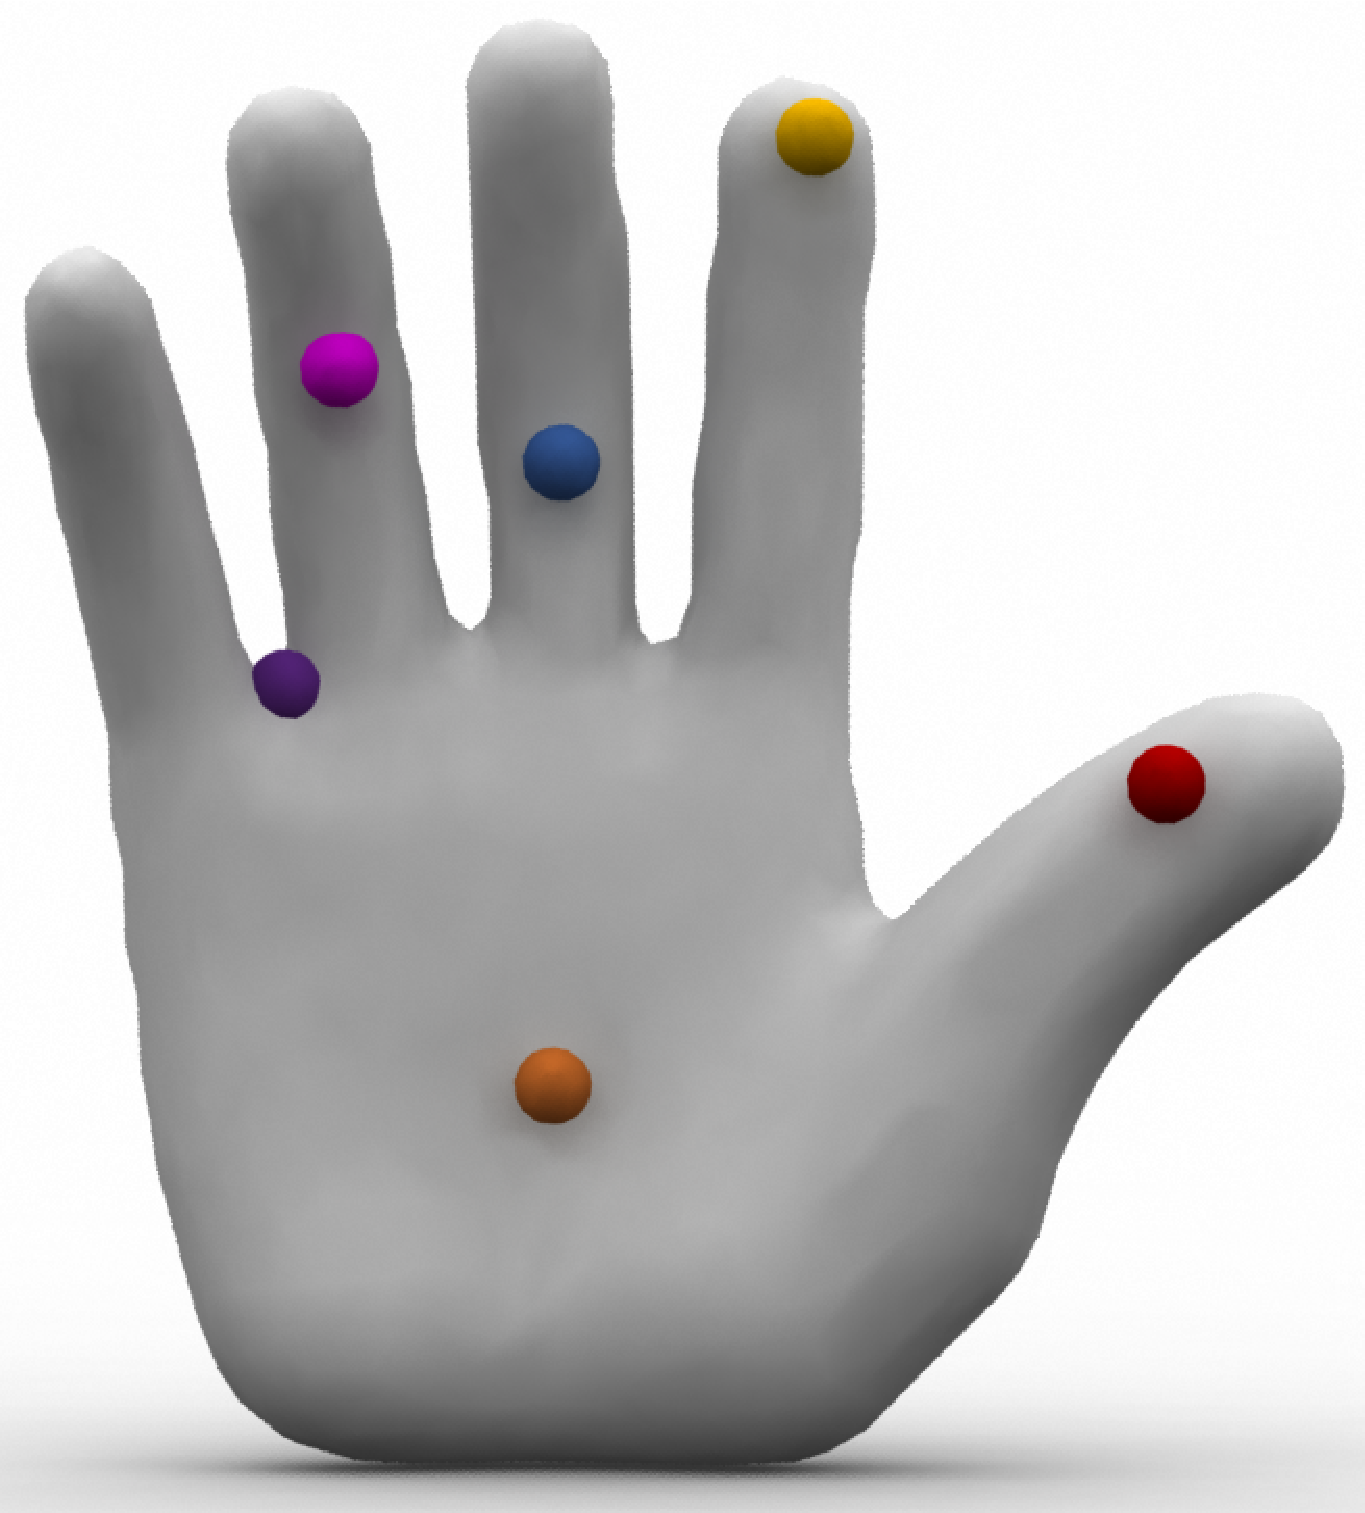
\includegraphics[height=.11\linewidth]{figures/surface_maps/source_hands.pdf}
\!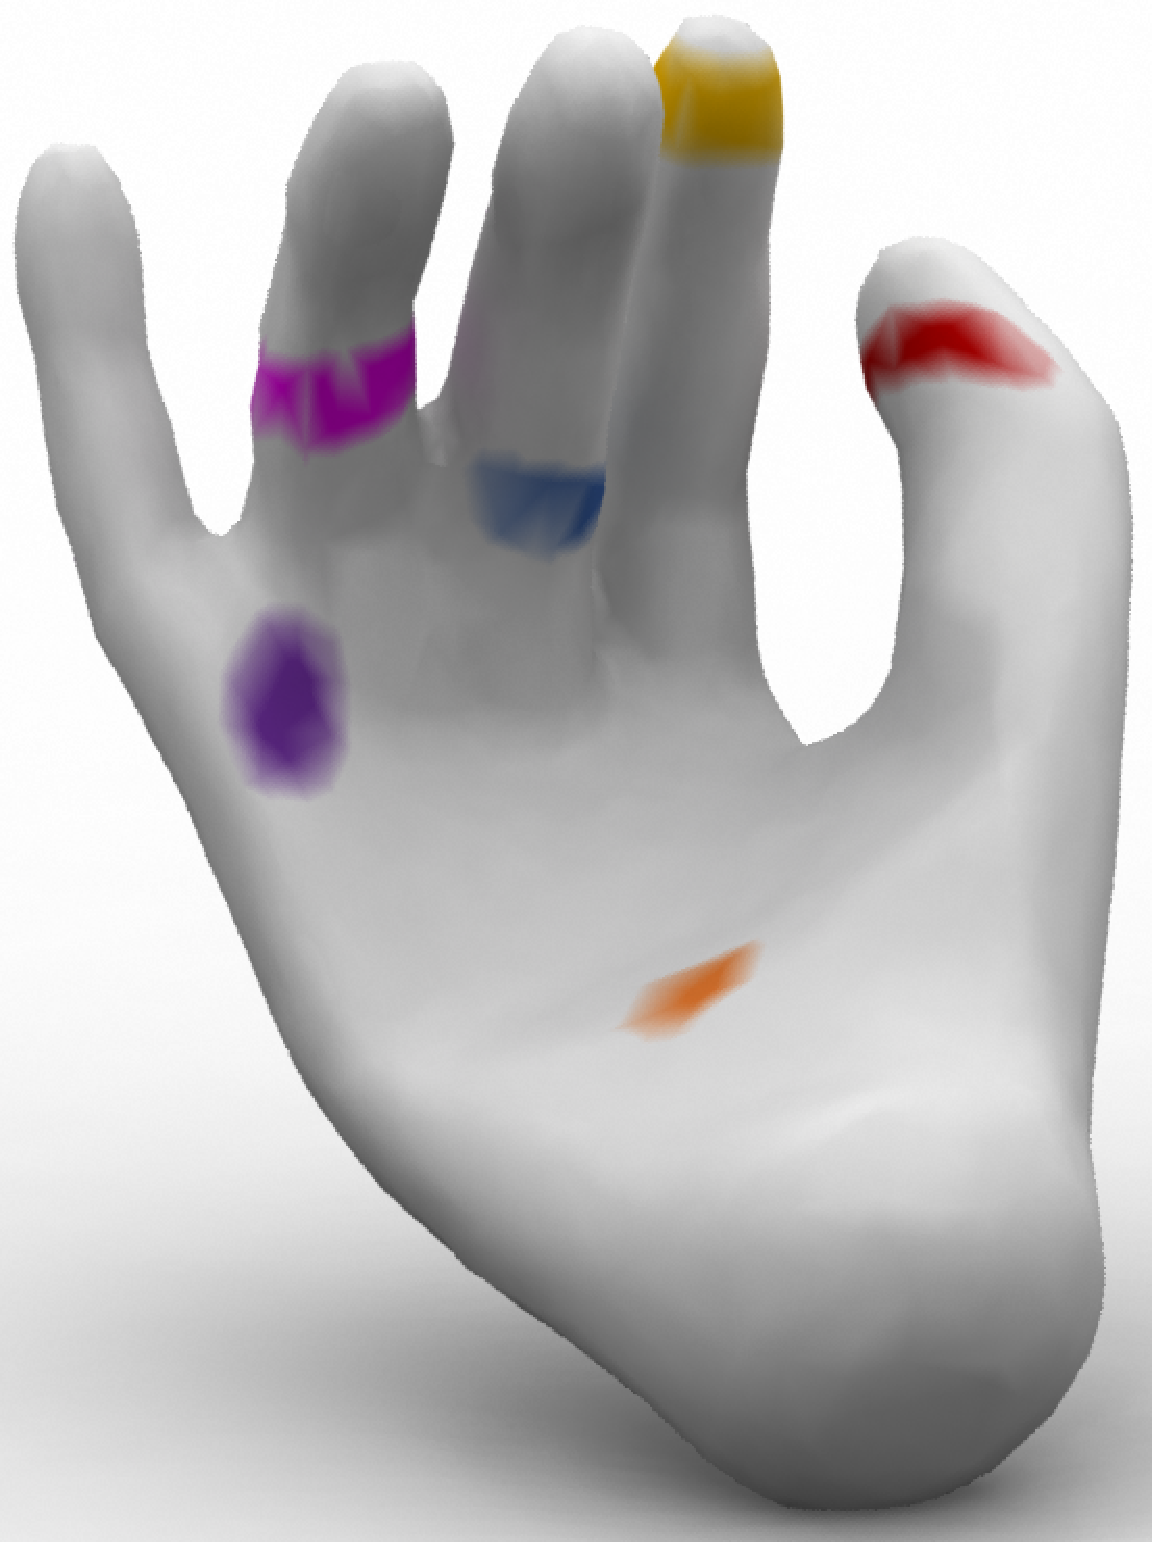
\includegraphics[height=.11\linewidth]{figures/surface_maps/target_hands.pdf}
\!}
\fbox{
\!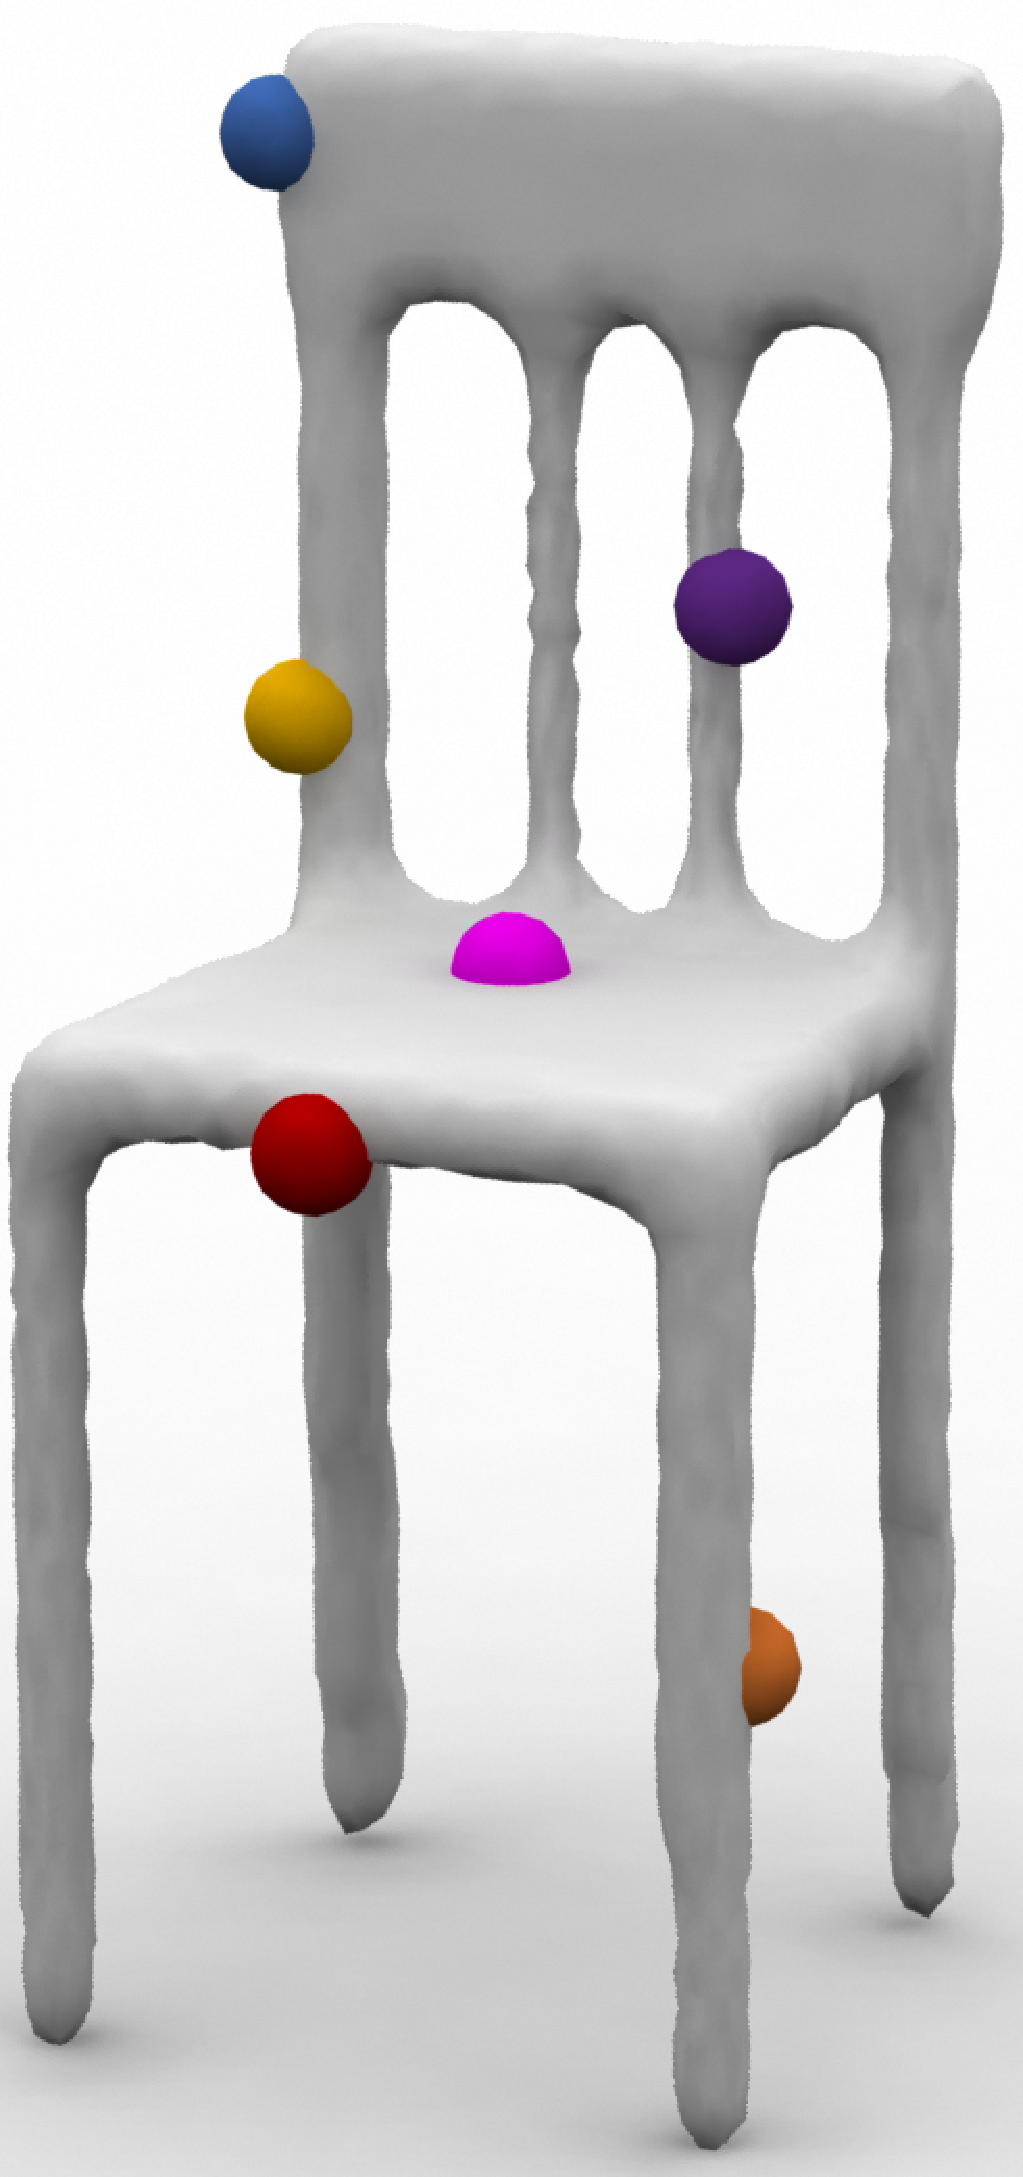
\includegraphics[height=.15\linewidth]{figures/surface_maps/source_chair.pdf}
\!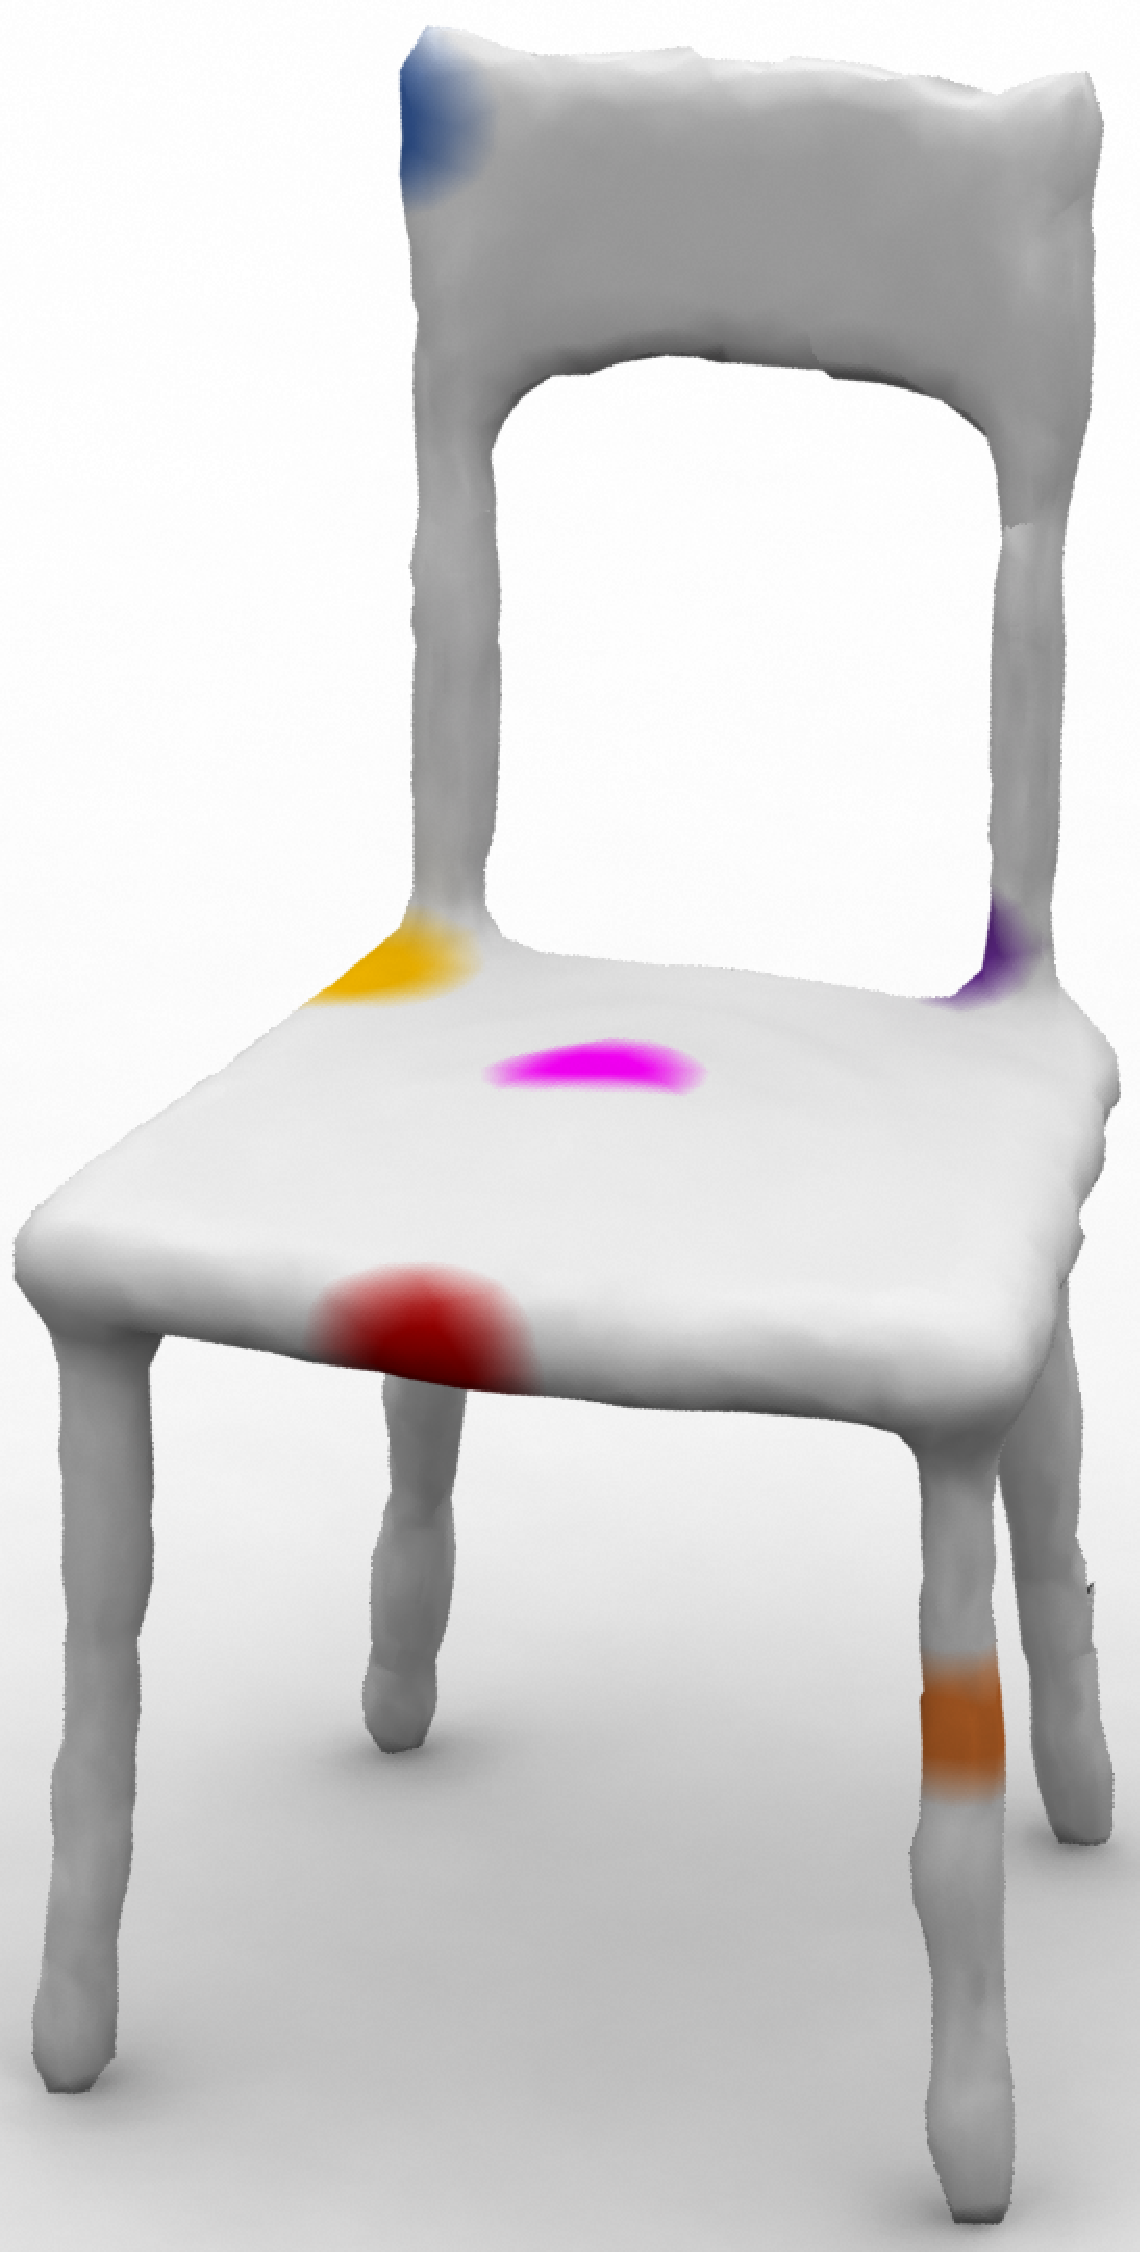
\includegraphics[height=.15\linewidth]{figures/surface_maps/target_chair.pdf}
\!}
\fbox{
\!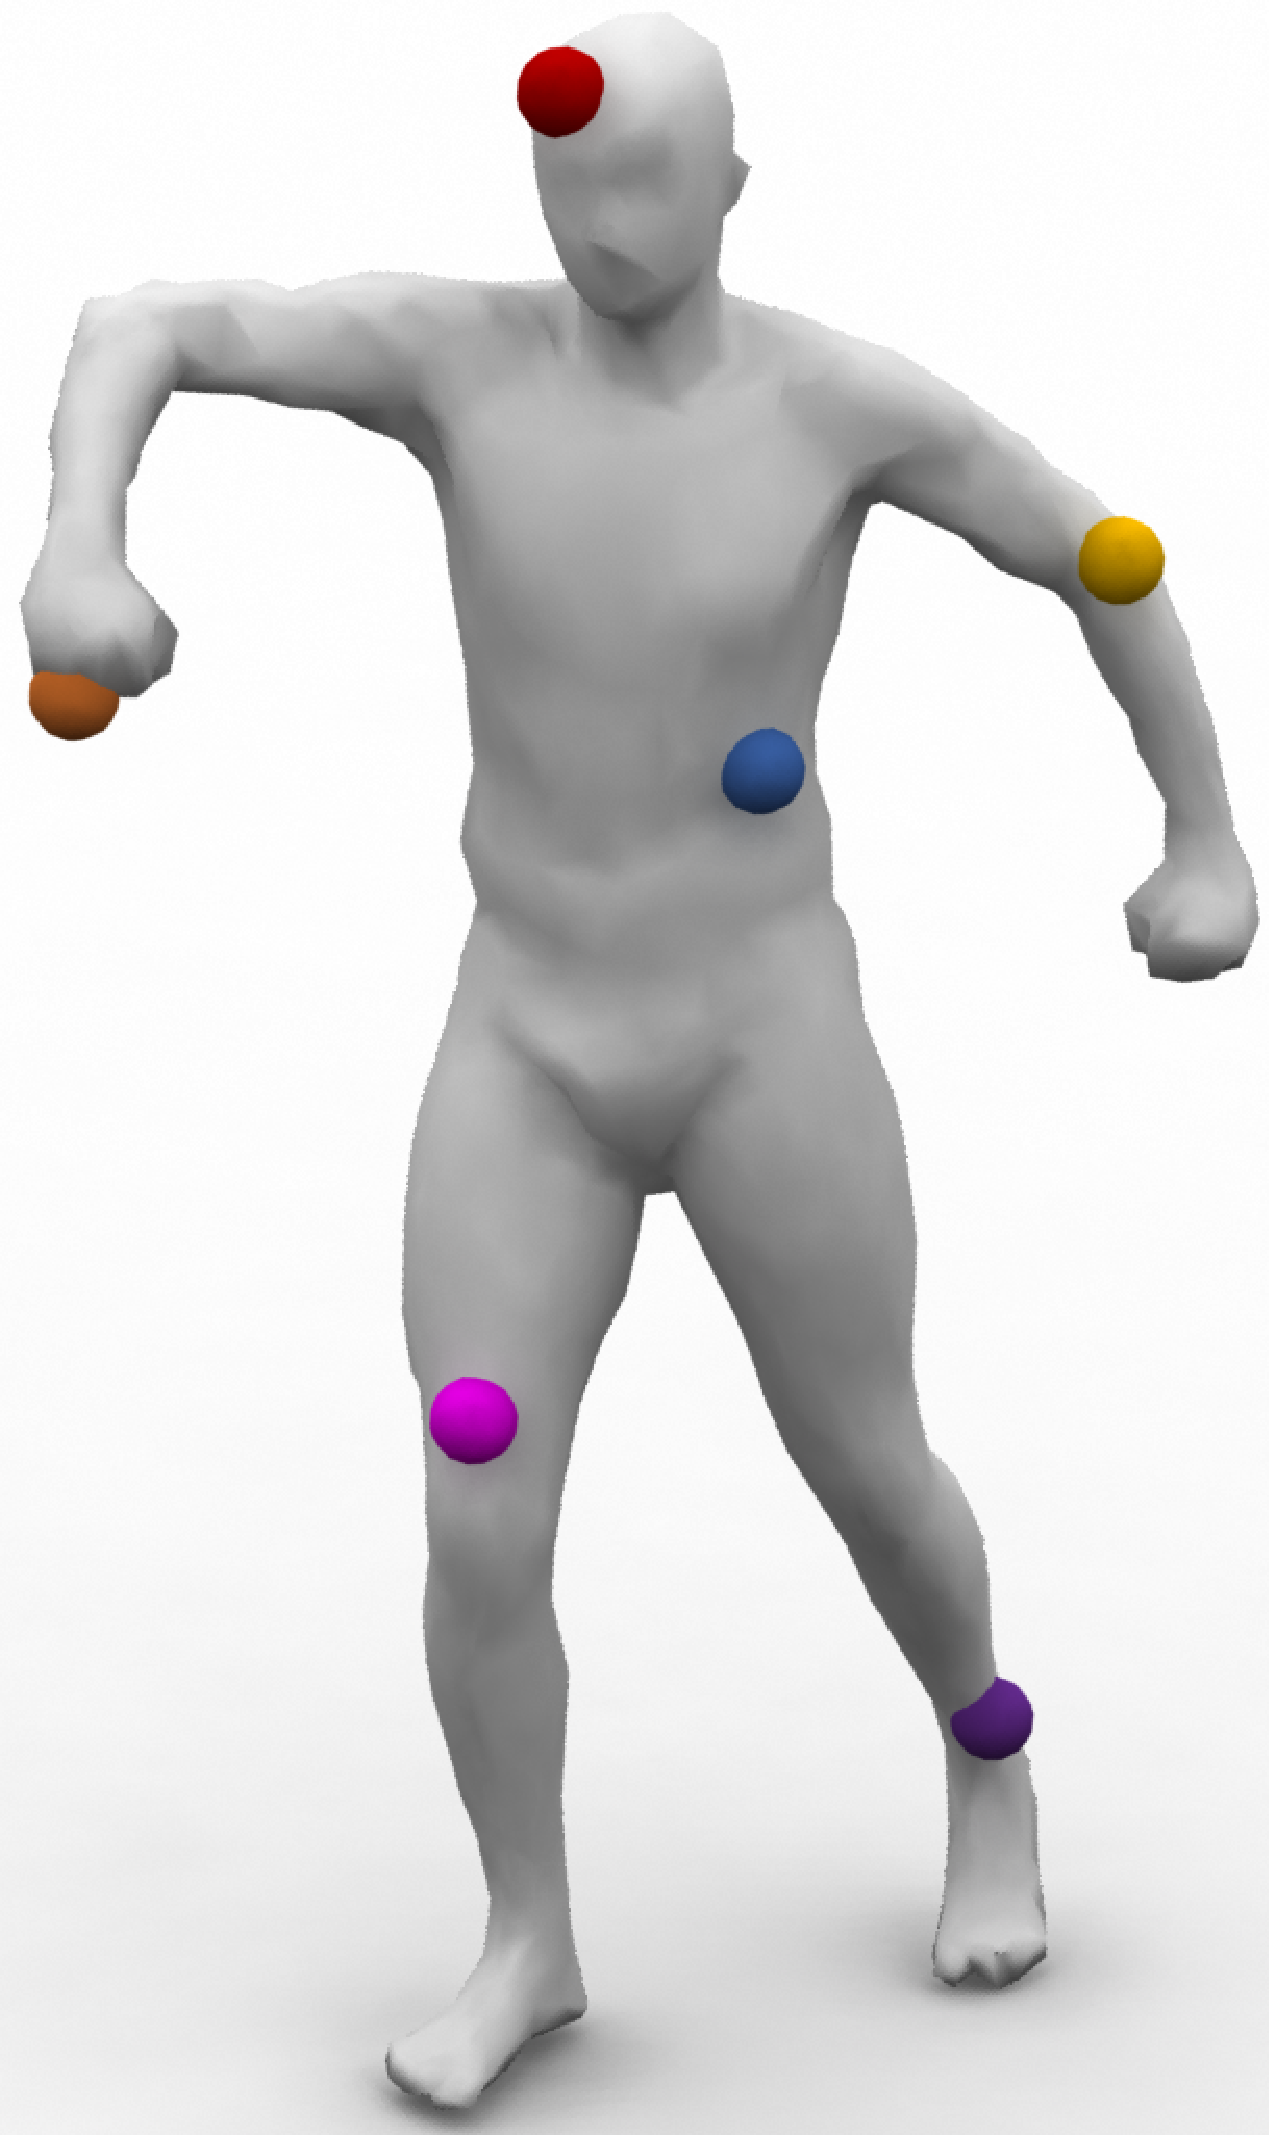
\includegraphics[height=.15\linewidth]{figures/surface_maps/source_human.pdf}
\!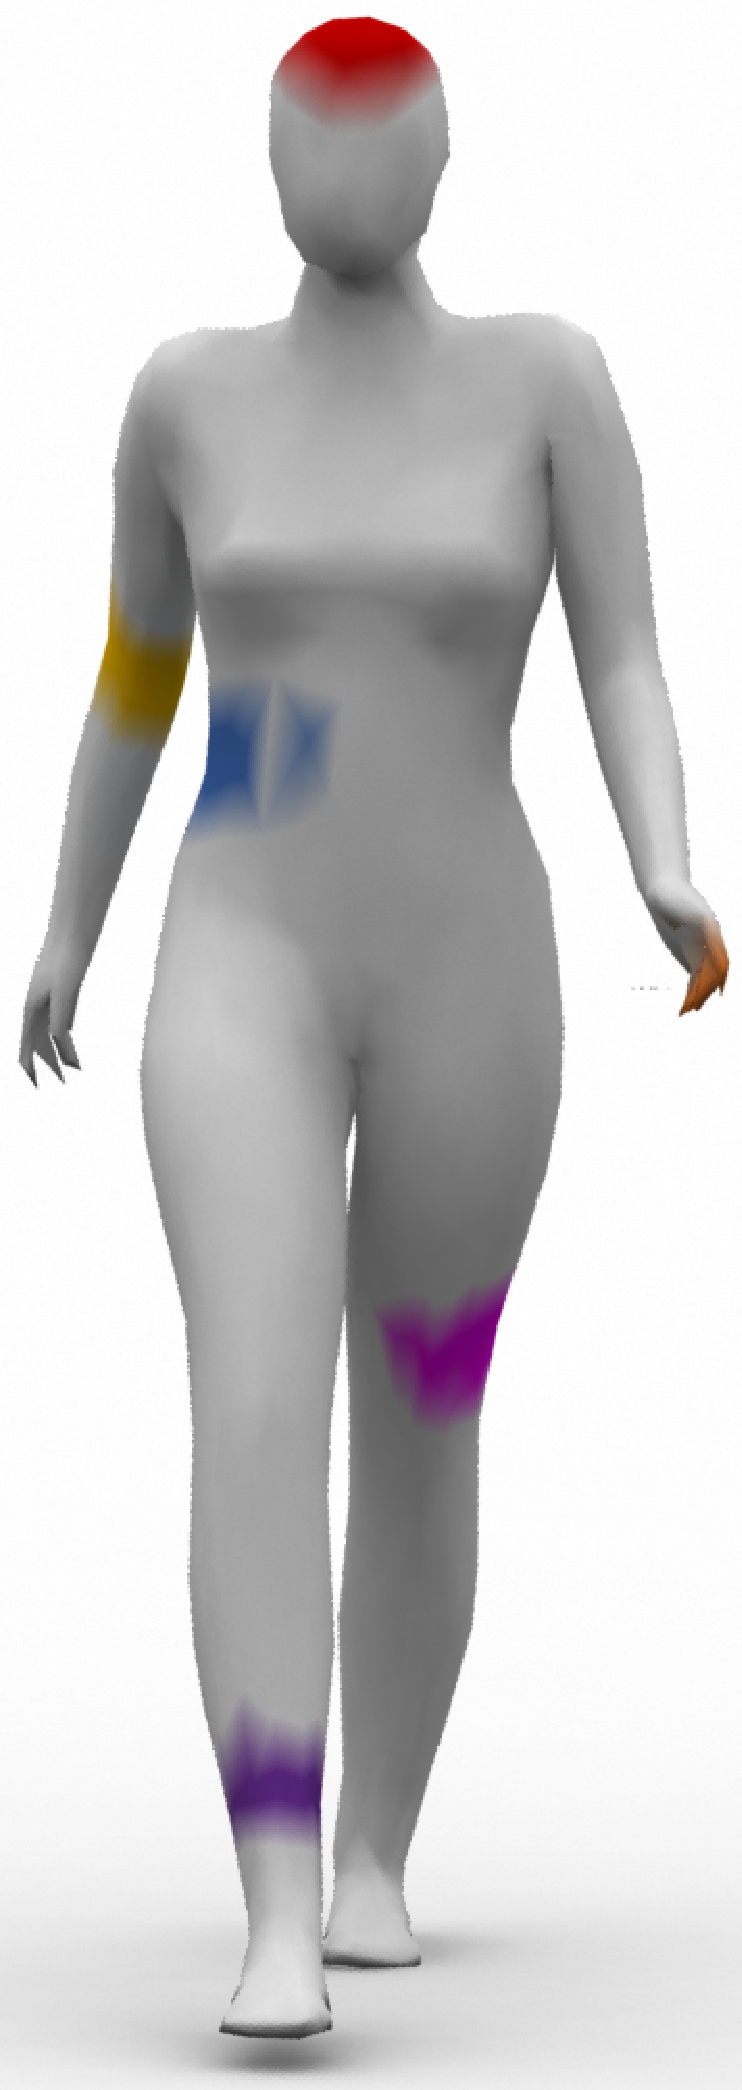
\includegraphics[height=.15\linewidth]{figures/surface_maps/target_human.pdf}
\!}
\fbox{
\!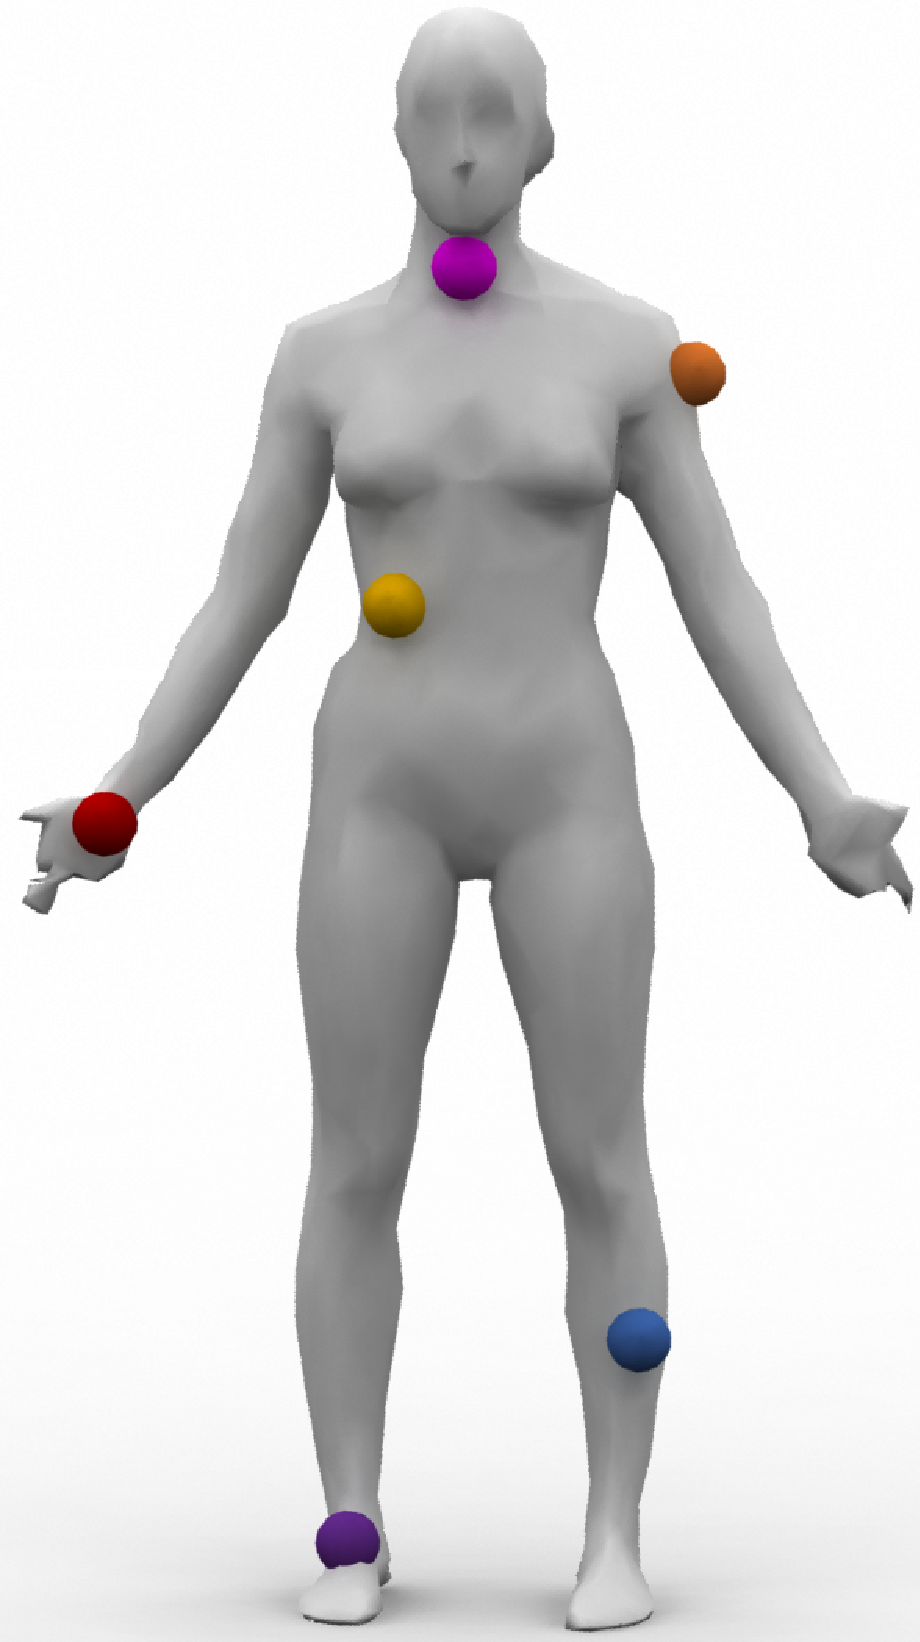
\includegraphics[height=.15\linewidth]{figures/surface_maps/source_humantostick.pdf}
\!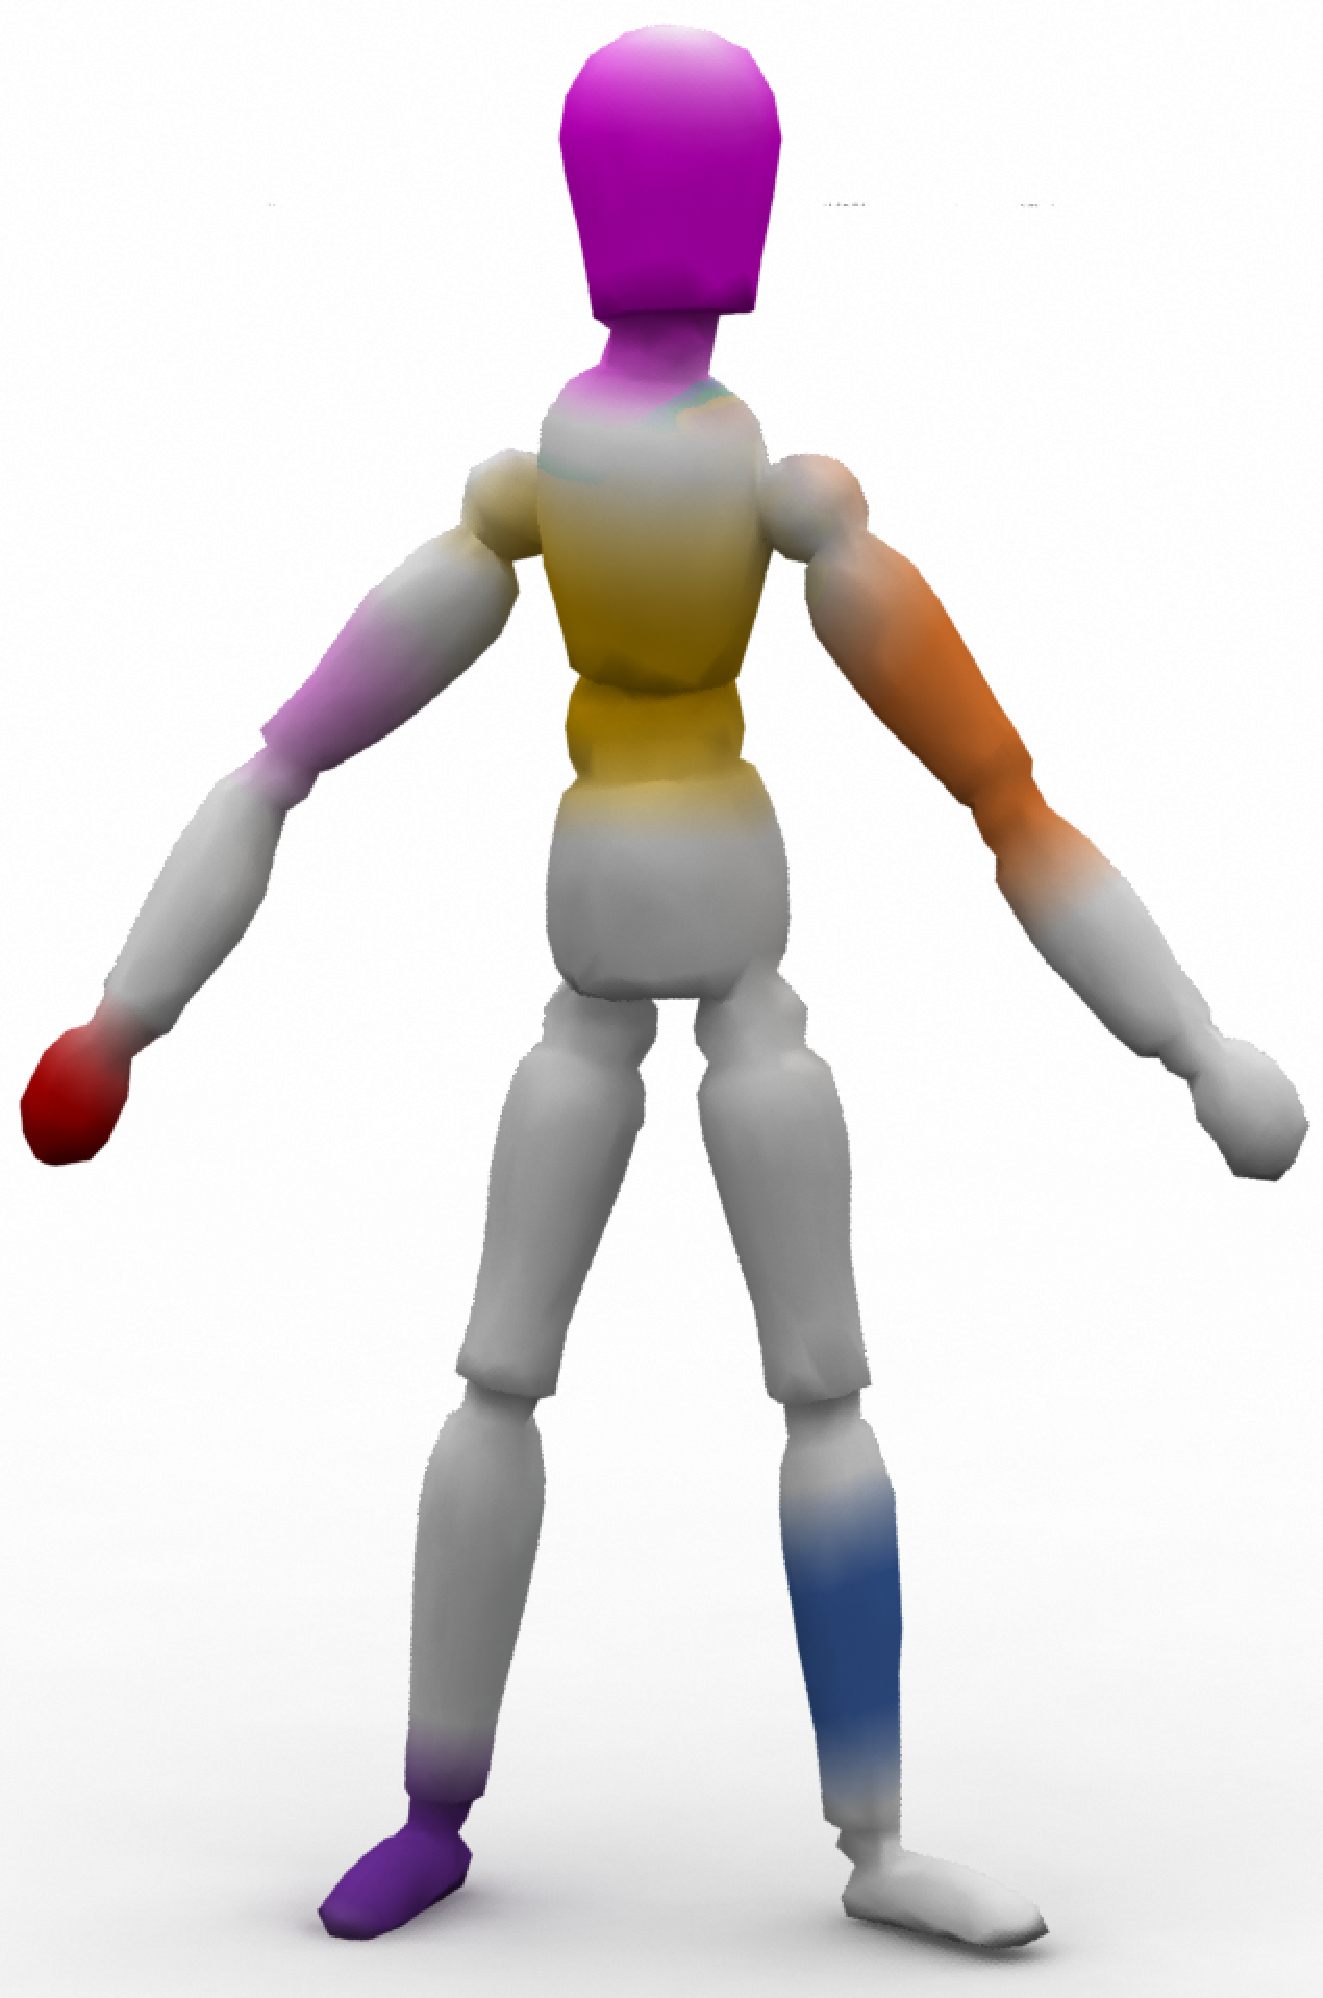
\includegraphics[height=.15\linewidth]{figures/surface_maps/target_humantostick.pdf}
\!}
\fbox{
\!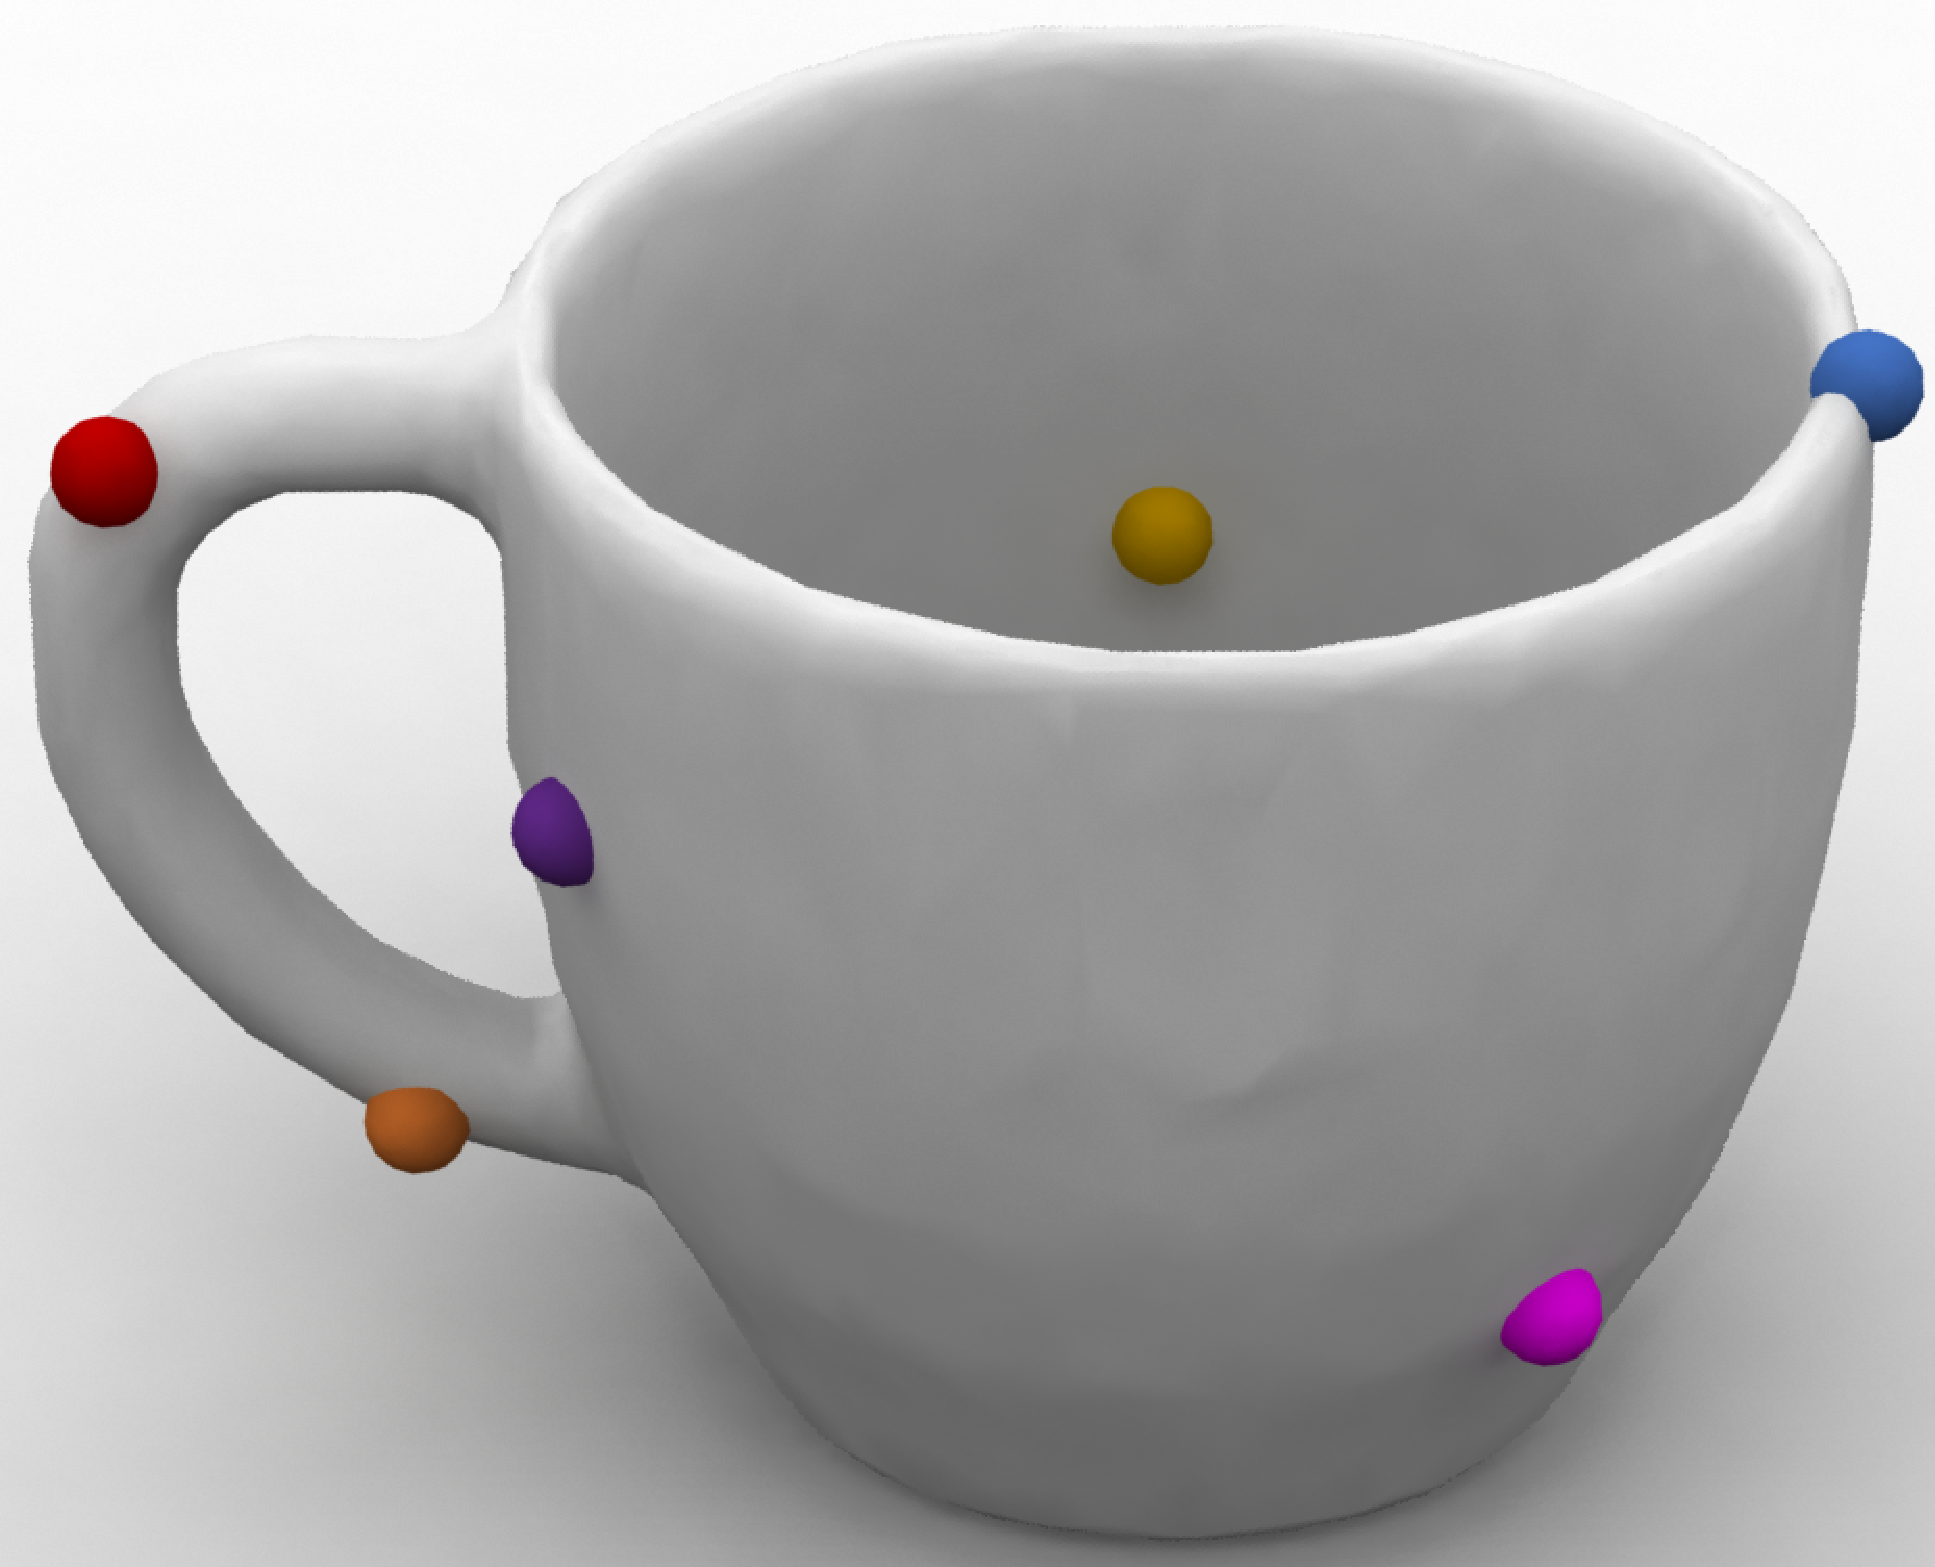
\includegraphics[height=.11\linewidth]{figures/surface_maps/source_mugs.pdf}
\!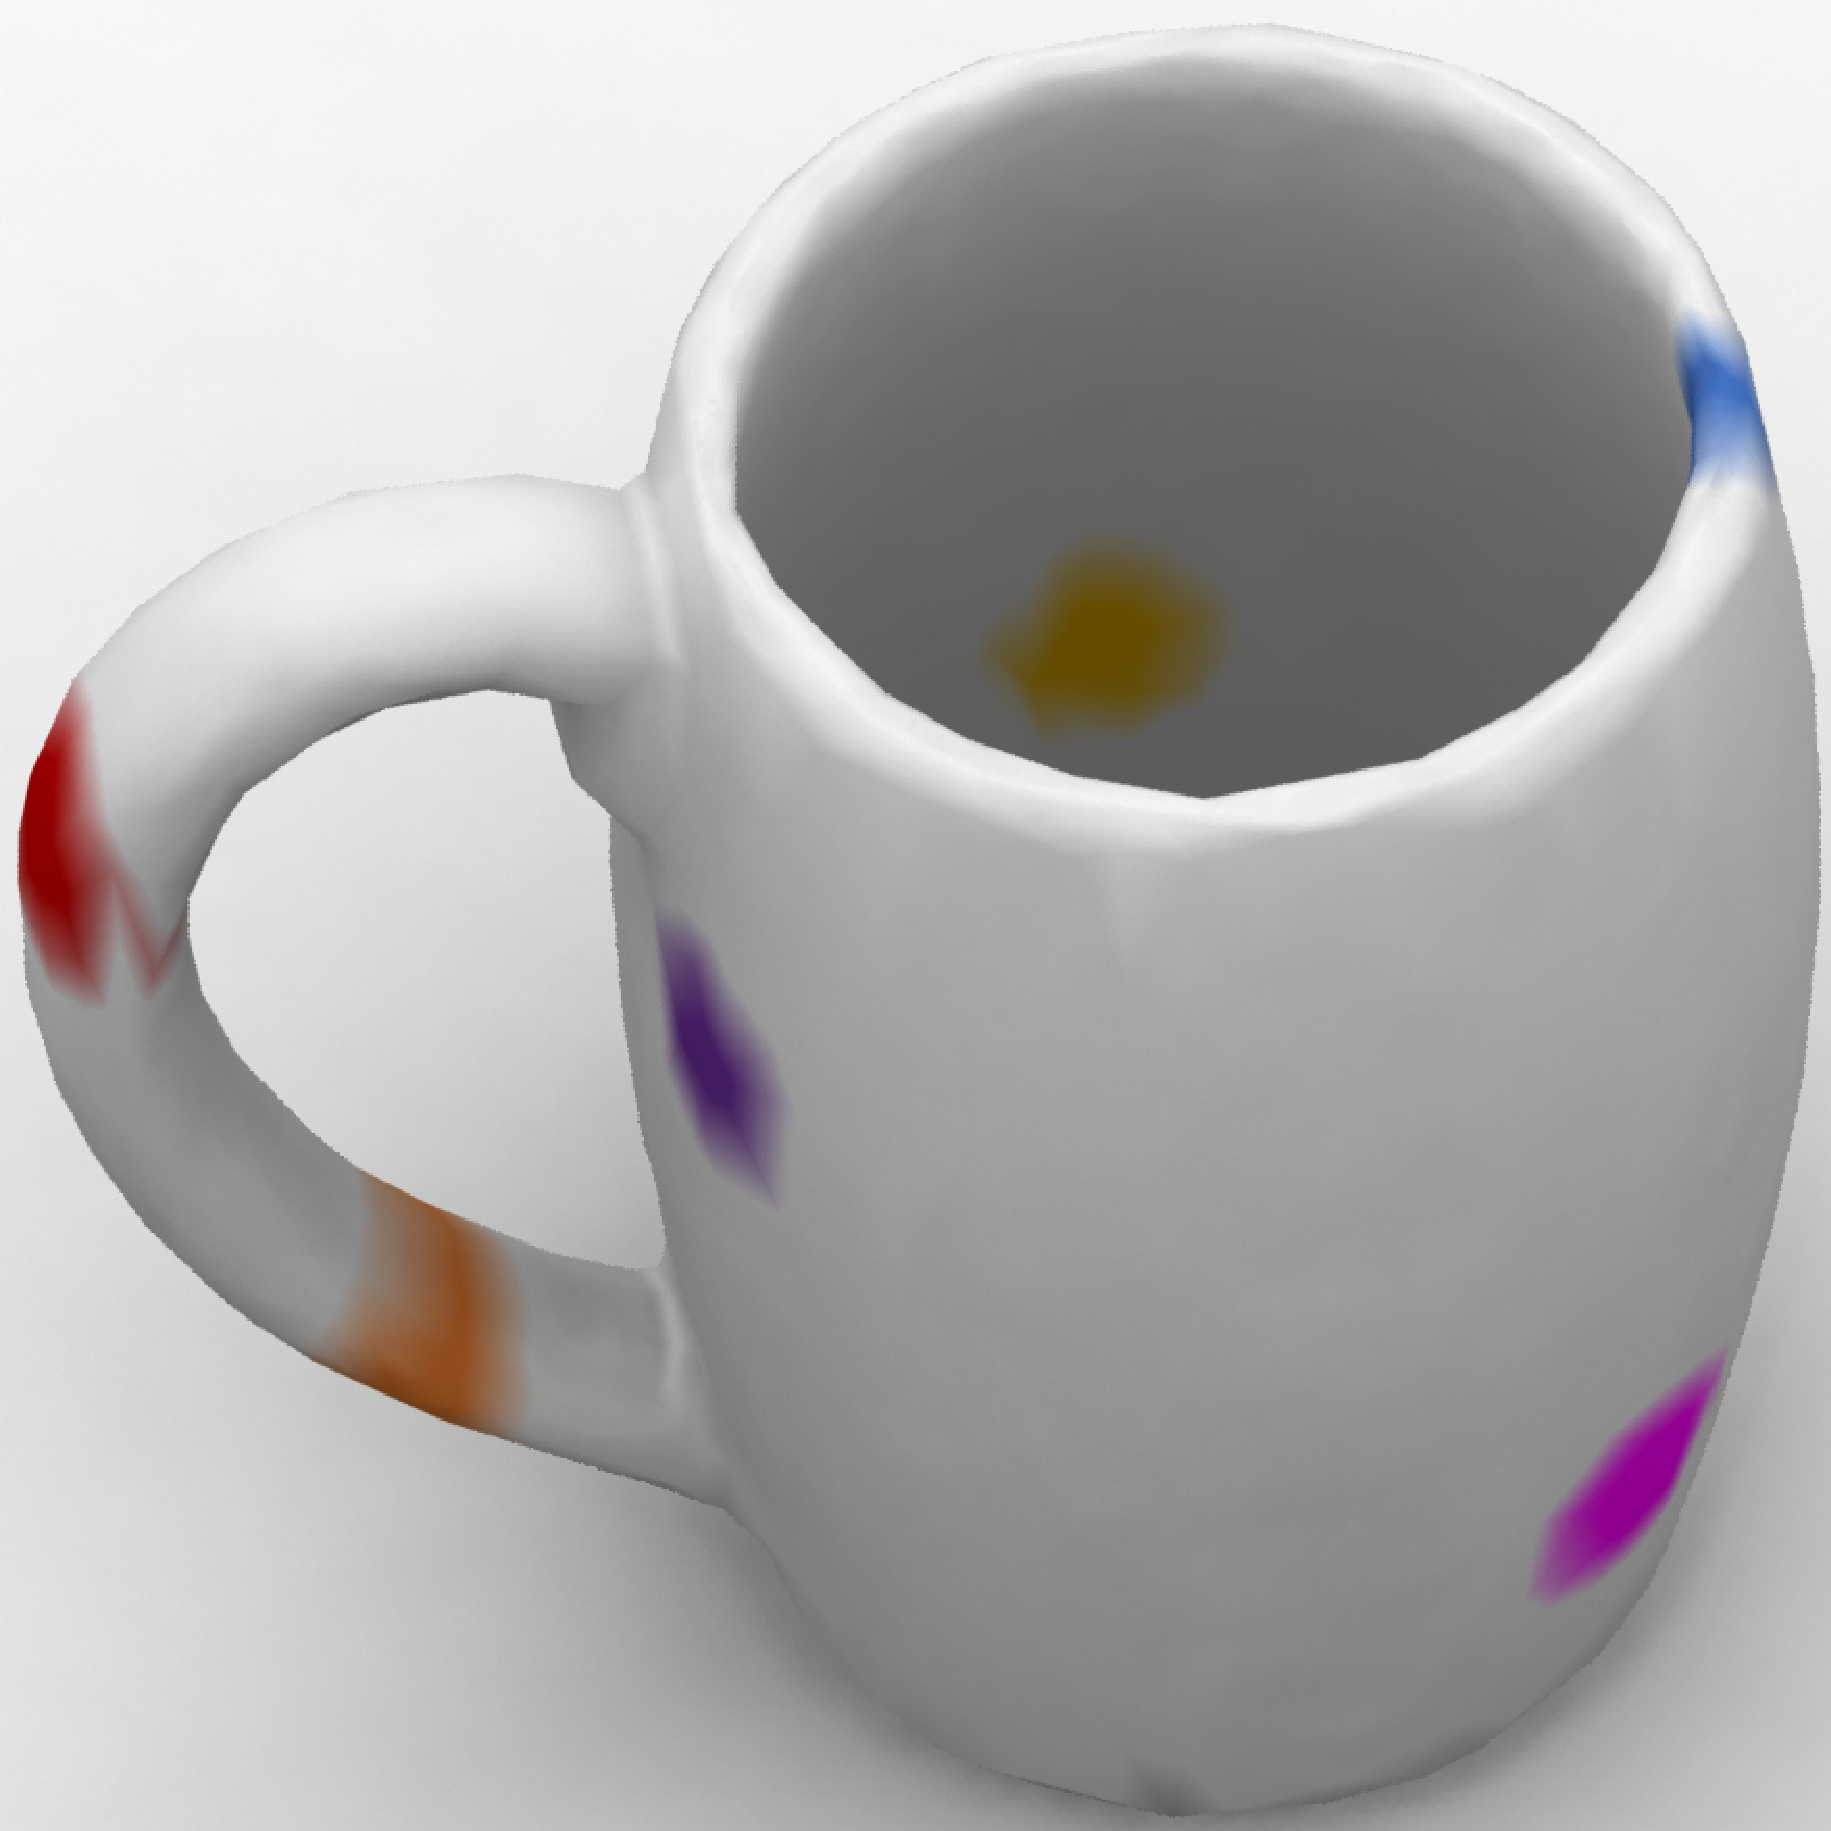
\includegraphics[height=.11\linewidth]{figures/surface_maps/target_mugs.pdf}
\!}
\caption{Additional surface correspondences computed using Algorithm~\protect\ref{alg:gw} ($\alpha\!\equiv\!5\!\times\!10^{-4},\eta\!\equiv\!1$).  As in~\protect\cite{solomon-2015},  colored points on the left are mapped to colored distributions on the right.  \S\ref{sec:symmetry} details a method for addressing the symmetry reversal in the third map.\vspace{-.15in}}\label{fig:more_maps}
\end{figure*}

\paragraph*{Generality.} Throughout this paper, we attempt to demonstrate our algorithm on a variety of matching tasks.  In this section, we highlight a few additional examples to underscore its wide applicability.

%\begin{figure}[t]\centering % became the teaser
%\begin{tabular}{c@{\hspace{.25in}}c}
%\includegraphics[height=.5\linewidth]{figures/icon/icon_source.pdf}&
%\includegraphics[height=.5\linewidth]{figures/icon/icon_target.pdf}
%\end{tabular}
%\caption{Mapping a 3D model onto a 2D icon ($n_0\!=\!2002,n\!=\!2315,\alpha\!=\!3\times10^{-5}$).}\label{fig:shape_to_icon}
%\end{figure}
Figure~\ref{fig:shape_to_icon} (page 1) tests our algorithm's flexibility to domain class.  Here, we map a triangle mesh to five different classes of target domains.  Despite the contrasting structures and even dimensionalities of the targets, our algorithm extracts a meaningful correspondence.

\begin{figure}[t]\centering
\begin{tabular}{c@{\hspace{.25in}}c}
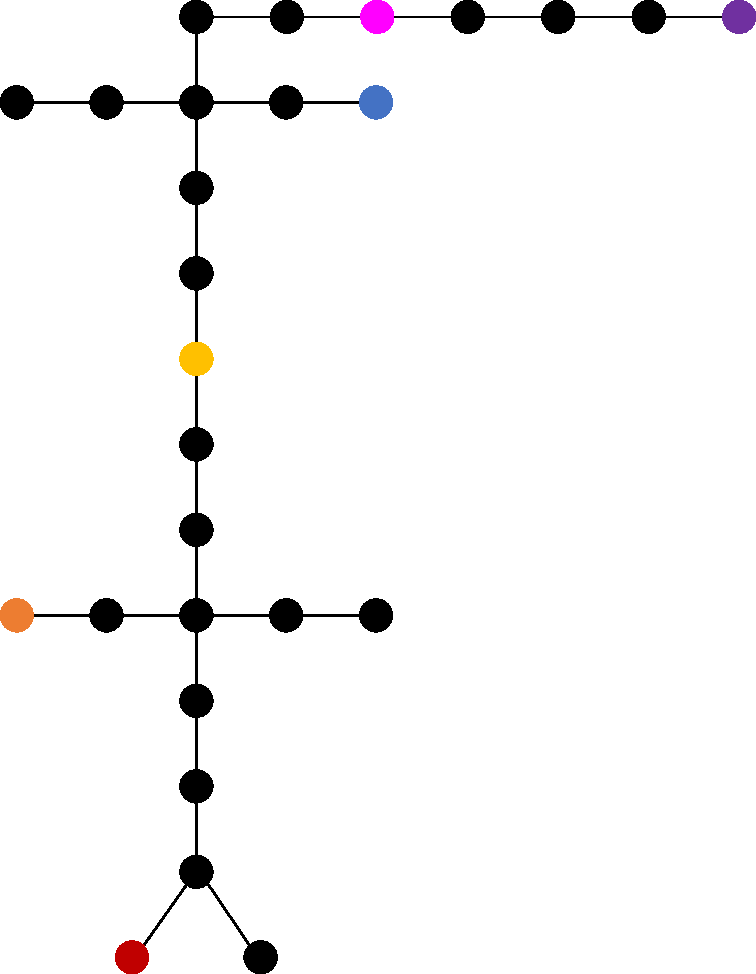
\includegraphics[height=.5\linewidth]{figures/graph_to_shape/graph.pdf}&
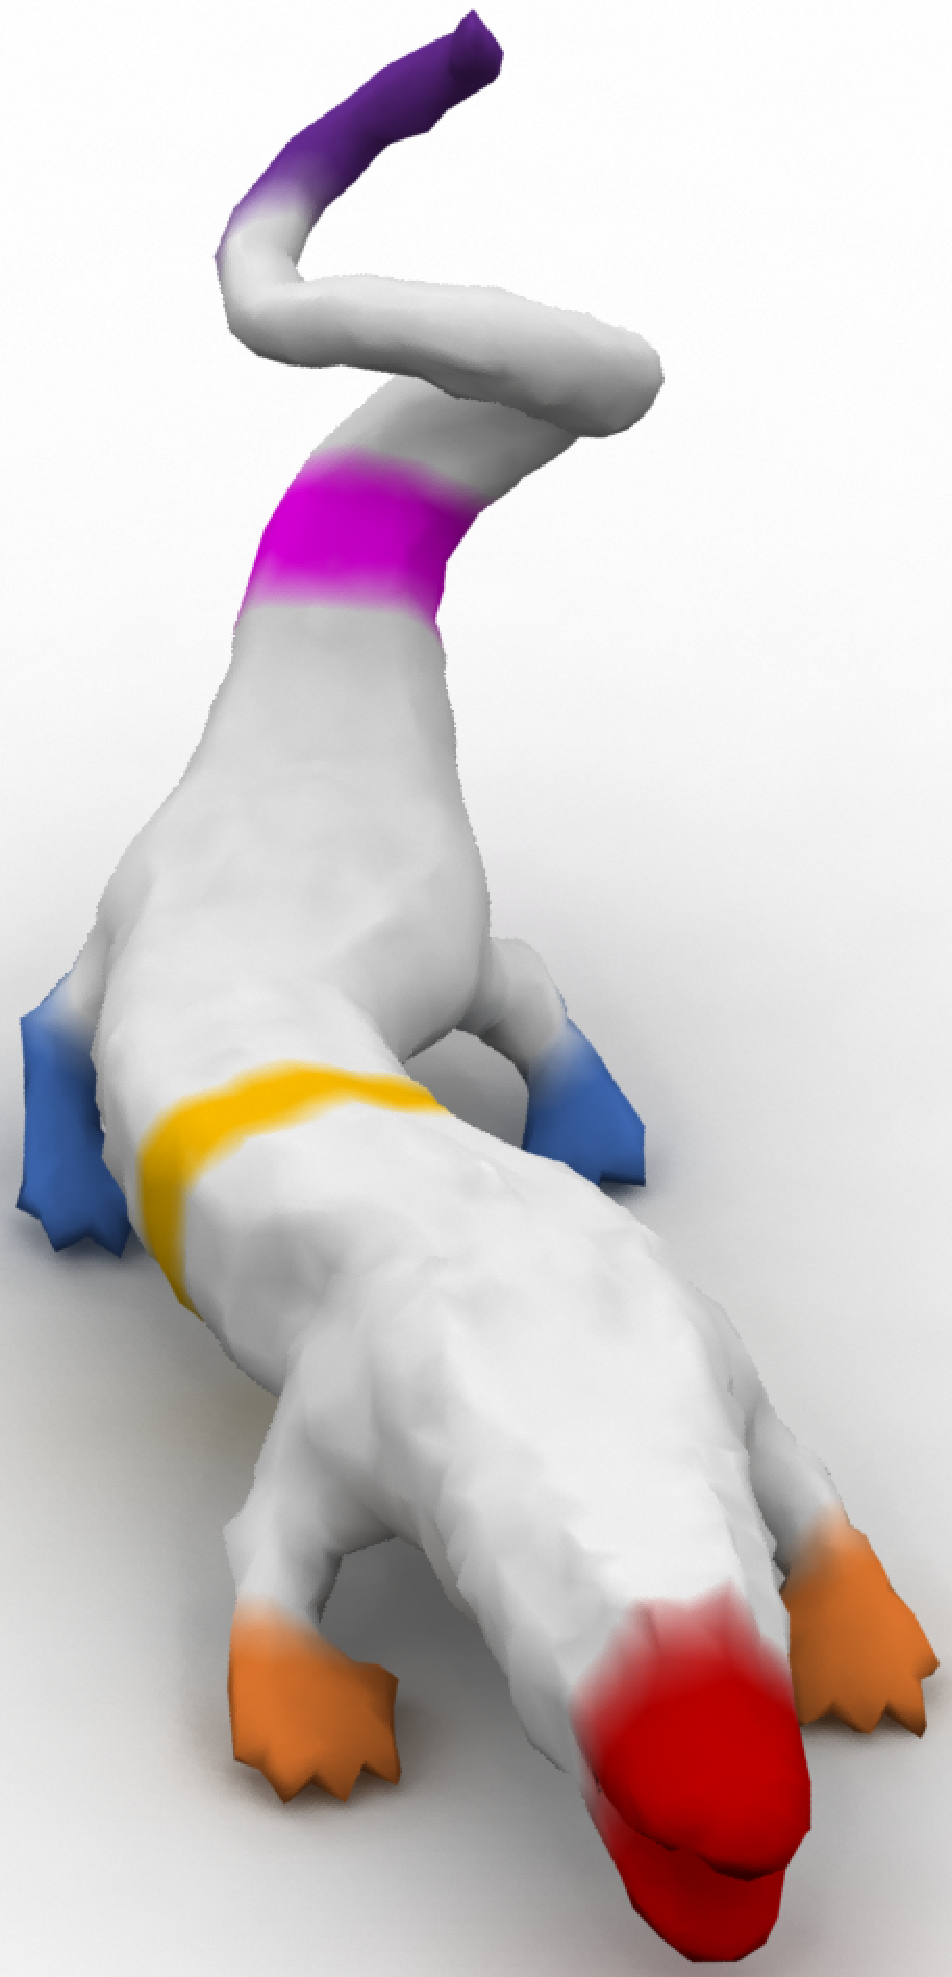
\includegraphics[height=.5\linewidth]{figures/graph_to_shape/alligator_target.pdf}
\end{tabular}
\caption{Mapping a graph onto a shape ($n_0\!=\!27,n\!=\!2502,\alpha\!=\!1.8\times10^{-4}$).\vspace{-.15in}}\label{fig:graph_to_shape}
\end{figure}
Similarly, Figure~\ref{fig:graph_to_shape} shows an example of mapping a graph onto a surface.  Here, distances $\D_0$ on the graph are all-pairs shortest-path distances with unit edge weights, and $\D$ contains geodesic distances on the target surface.  Convergence for this example was particularly fast given the small size of the source domain.

\begin{figure}[t]\centering
\includegraphics[height=\linewidth]{figures/image_grid/imageLayout.pdf}
\caption{Mapping 196 images onto a $14\times14$ image grid while preserving color similarity. \small{(Images from Flickr public domain collection.)}\vspace{-.15in}}\label{fig:images}
\end{figure}

Figure~\ref{fig:images} applies our machinery to mapping a set of images onto a grid layout; as a point of comparison, Fried et al.~\shortcite{fried-2015} recently proposed a more complicated optimization routine for the same problem.  Here, $\D_0$ contains distances between average \textsc{Lab} color over an image, and $\D$ contains Euclidean distances between grid cells.  For this application, we need to extract a matching rather than a soft measure coupling $\G$.  To do so, after optimizing for $\G$, we solve a linear assignment problem
$$
\begin{array}{rl}
\max_{\tilde\G} & \langle \tilde \G,\G\rangle\\
\textrm{s.t.} & \tilde\G\geq0\\
&\tilde\G\1=\1n\hspace{.25in}\tilde\G^\top\1=\1n_0.
\end{array}
$$
When $n_0=n$, this linear program admits a permutation matrix solution computable using a standard convex optimization tool or any of the many fast solvers for assignment problems.%\suv{Or using any of the 10s of fast solvers that exist for assignment problems.}

\setlength{\columnsep}{2pt}
\begin{wrapfigure}[9]{r}{0.23\textwidth}\centering
\vspace{-.15in}
\begin{tabular}{c@{}c}
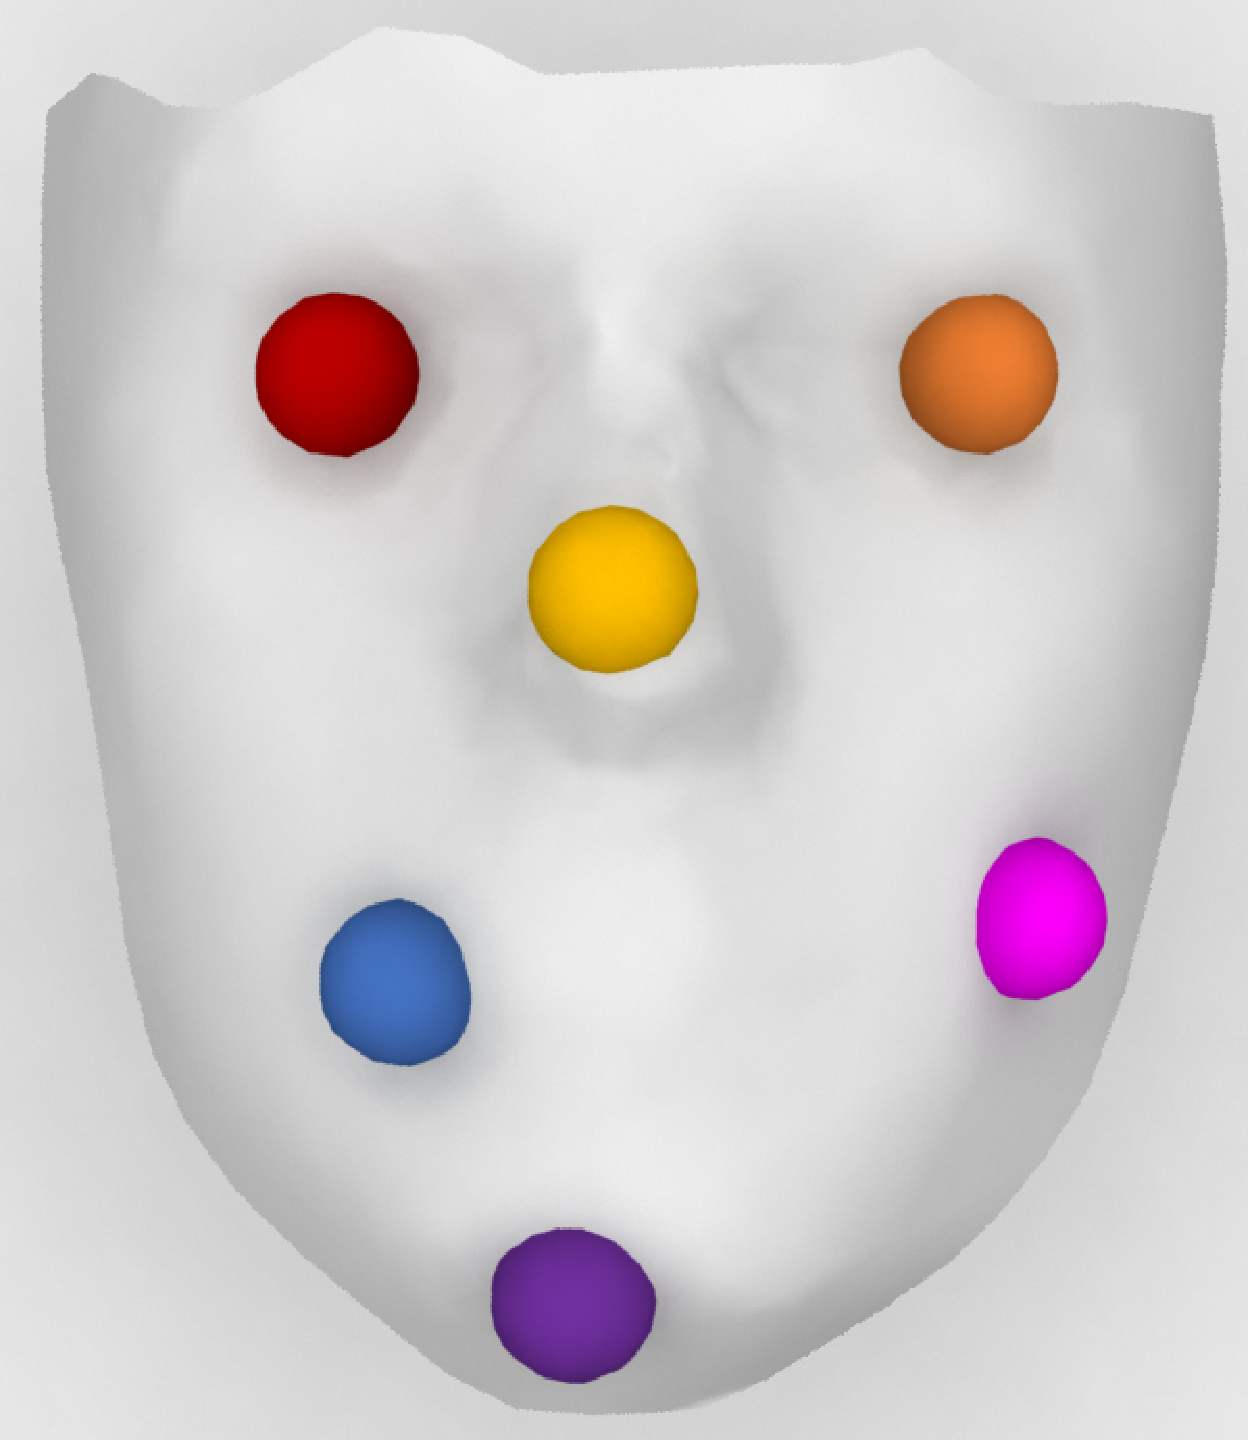
\includegraphics[height=.6\linewidth]{figures/cloud/source_cloud.pdf}&
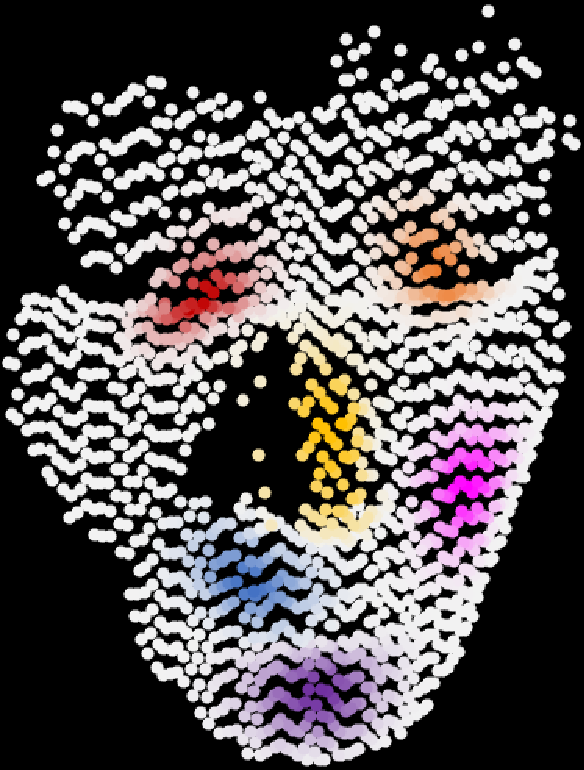
\includegraphics[height=.6\linewidth]{figures/cloud/cloud.pdf}
\end{tabular}
\vspace{-.15in}
\caption{Point clouds.}\label{fig:clouds}
\end{wrapfigure}
Figure~\ref{fig:clouds} shows an example matching a triangle mesh to a point cloud.  Here, we match a noisy and sparse point cloud face scan to a generic mesh of a face. Since the two shapes are in approximately the same pose, we take $\D_0, \D$ to contain Euclidean (rather than geodesic) distances.  We use mesh-based area weights on the source and uniform area weights on the target.  The match is successful despite the nonuniform sampling of the point cloud and a missing patch on the nose.

%\begin{figure}[t]\centering
%\fbox{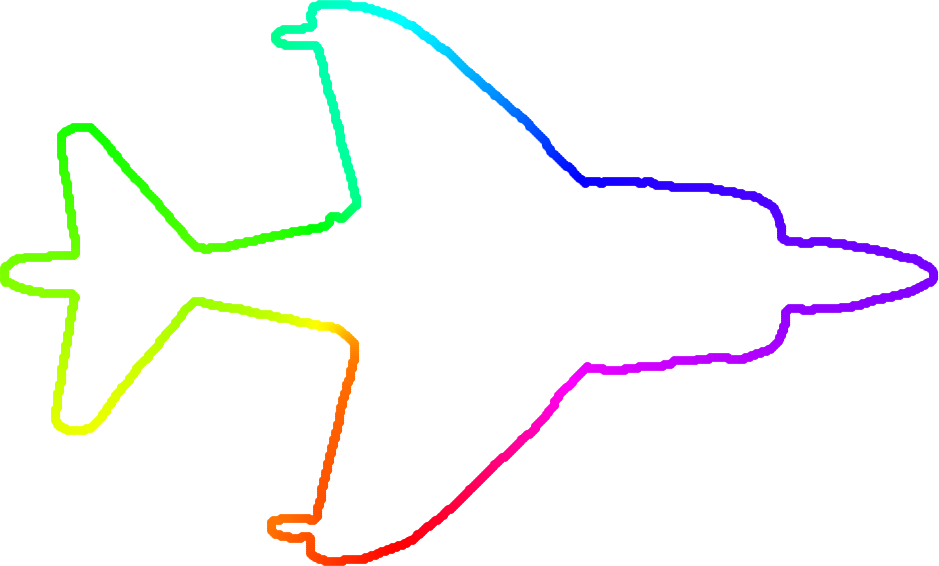
\includegraphics[scale=.1]{figures/2d_shape_match/source.pdf}}\ \ \foreach \n in {1,...,4}{\includegraphics[scale=.09]{figures/2d_shape_match/target\n.pdf}\ \ }\\
%\fbox{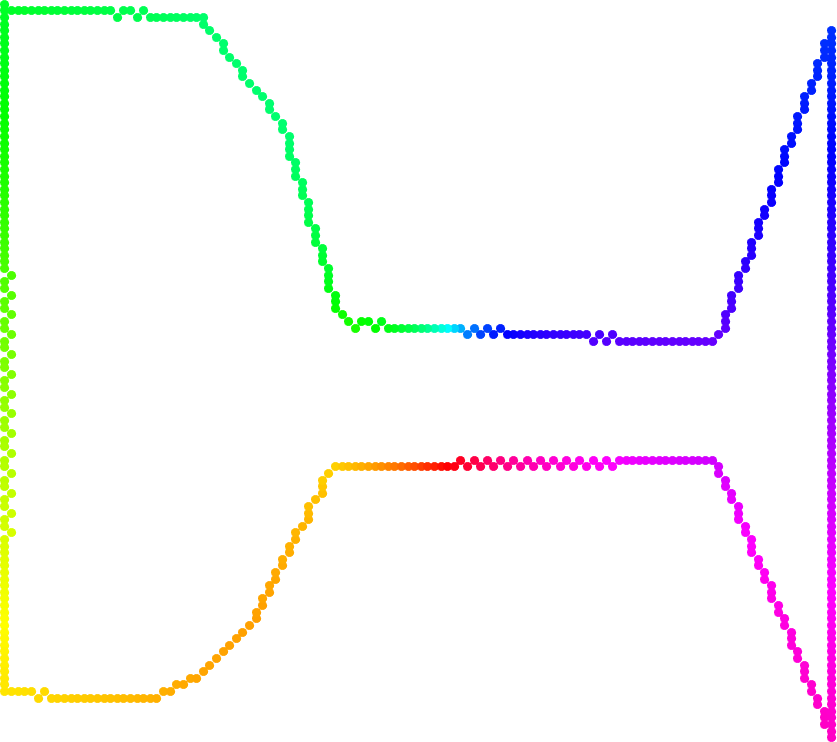
\includegraphics[scale=.1]{figures/2d_shape_match/source_glass.pdf}}\ \ \foreach \n in {1,...,4}{\includegraphics[scale=.1]{figures/2d_shape_match/target_glass\n.pdf}\ \ }\\
%\fbox{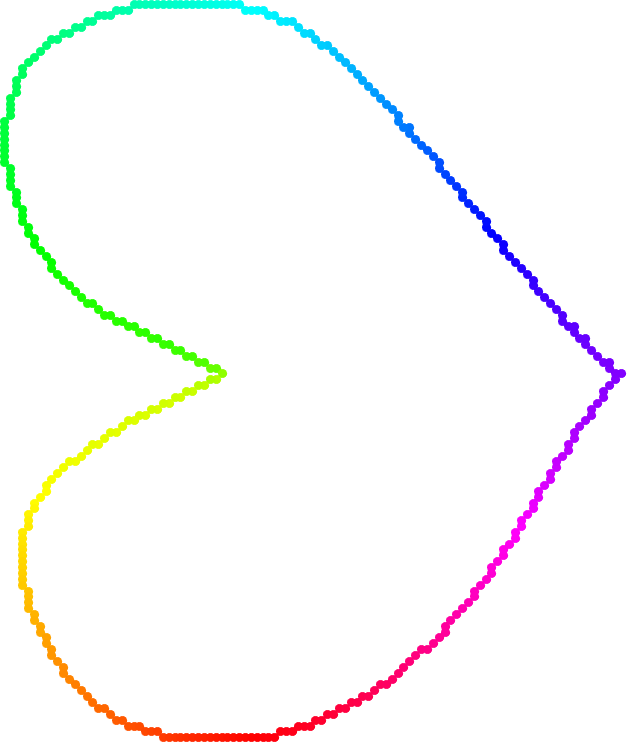
\includegraphics[scale=.1]{figures/2d_shape_match/source_heart.pdf}}\ \ \foreach \n in {1,...,4}{\includegraphics[scale=.12]{figures/2d_shape_match/target_heart\n.pdf}\ \ }\\
%\fbox{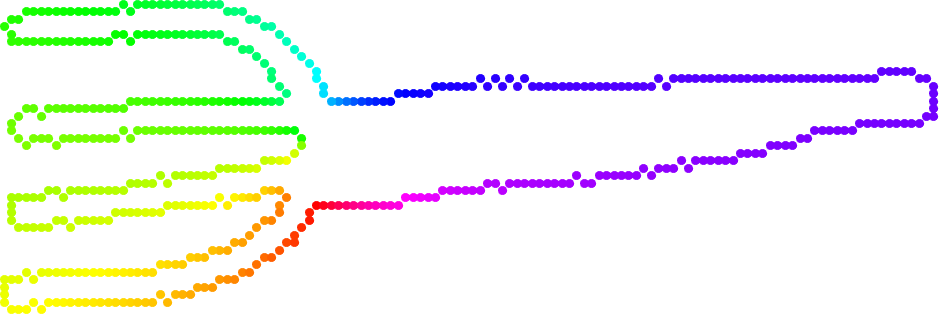
\includegraphics[scale=.1]{figures/2d_shape_match/source_fork.pdf}}\ \ \foreach \n in {1,...,4}{\includegraphics[scale=.1]{figures/2d_shape_match/target_fork\n.pdf}\ \ }
%\caption{2D shape matching; color on the boxed model is transferred to the remaining models ($\alpha\equiv7.5\times10^{-4}$); results on full dataset in supplemental material.}\label{fig:2d_shape}
%\end{figure}

\setlength{\columnsep}{2pt}
\begin{wrapfigure}[7]{r}{0.12\textwidth}\centering
\vspace{-.15in}
\begin{tabular}{cc}

\includegraphics[height=.9\linewidth]{figures/2d_shape_match/source_fuzzy_fork.pdf}&

\includegraphics[height=.9\linewidth]{figures/2d_shape_match/target_fuzzy_fork.pdf}
\end{tabular}
\vspace{-.15in}
\caption{}\label{fig:forks}
\end{wrapfigure}
%Figure~\ref{fig:2d_shape} shows 
The supplemental document includes a 2D shape matching test (data from~\cite{thakoor-2007}).  The shapes are point clouds without topology.  We use the rounding procedure outlined for image layout to display the maps, transferring colors from the matched point on a source shape (boxed). Our algorithm recovers smooth maps for most 2D test cases.  The most challenging test in the dataset is the ``fork'' class; these shapes admit symmetries \emph{and} thin structures that make it difficult to extract a point-to-point map after applying the entropic regularizer.  Figure~\ref{fig:forks} shows an example before rounding.

%\paragraph*{Validation.} \justin{Hoping Vova can think of some dataset to test on.}

\paragraph*{Comparison.}  Here we provide a few examples qualitatively demonstrating how our method differs from existing work.

\begin{figure}[t]\centering\renewcommand{\arraystretch}{0.8}% Tighter
\begin{tabular}{@{}c@{\hspace{.1in}}c|c@{\hspace{.1in}}c@{}}
\includegraphics[height=.13\linewidth]{figures/sdp/sdp1.pdf}&
\includegraphics[height=.17\linewidth]{figures/sdp/sdp2.pdf}&
\includegraphics[height=.13\linewidth]{figures/sdp/gw1.pdf}&
\includegraphics[height=.17\linewidth]{figures/sdp/gw2.pdf}\\
Test 1 & Test 2 & Test 1 & Test 2\\
\tiny$\lambda_1\!=\!7,\lambda_2\!=\!0$
&
\tiny$\lambda_1\!=\!4,\lambda_2\!=\!3$
&
\tiny 6 iterations
&
\tiny 14 iterations
\\\hline
\multicolumn{2}{|c|}{\small \cite{kezurer-2015}, 2499 variables}&
\multicolumn{2}{c|}{\small $\GWa$, $\alpha\!=\!10^{-3}$, 49 variables}\\\hline
\end{tabular}
\caption{Comparison to SDP matching.  The points on the left of the vertical dotted lines are mapped to the right; edge darkness indicates value of $\G$.  The two largest eigenvalues are shown for~\protect\cite{kezurer-2015}; the second test case is not tight.  The number of iterations for six digits of precision is shown for \GWa.}\label{fig:sdp}
\end{figure}
Figure~\ref{fig:sdp} compares to~\cite{kezurer-2015} for a 2D matching problem using pairwise Euclidean distances.  We show a symmetric test case and an asymmetric test case.  For fair comparison, we use their SDP relaxation on the GW objective.  Our unoptimized implementation instantiated 2499 variables to match seven points using their method, which has $O(n^4)$ variables for $n$ matched points.  Beyond an obvious difference in timings, their relaxation was not tight in the symmetric test.  %; in their notation, the output  satisfied $Y\neq[X][X]^\top$.  
While optimization via the interior point method recovered a map that arbitrarily superposed the two equally optimal maps, the weights of the superposition were not isotropic or controllable.  Our method recovered a sharp map; the symmetric map can be recovered as described in \S\ref{sec:symmetry}.

The supplemental document includes a comparison to~\cite{aflalo-2015} in which we minimize $\|\D_0\G-\G\D\|_{\mathrm{Fro}}$ over doubly stochastic $\G$.  To match their setup, we assume $n_0\!=\!n$ with uniform area weights.  Although their method does not require an SDP, the convexity of their objective is problematic for (nearly-)symmetric domains; see the supplemental document for discussion.

\setlength{\columnsep}{1pt}
\begin{wrapfigure}[10]{r}{0.3\textwidth}\centering\centering\renewcommand{\arraystretch}{0.8}% Tighter
\vspace{-.15in}
\begin{tabular}{@{}c@{}c@{}c@{}}
\includegraphics[height=.25\linewidth]{figures/bim/bimSource.pdf}&
\includegraphics[height=.5\linewidth]{figures/bim/bimTarget.pdf}&
\includegraphics[height=.5\linewidth]{figures/bim/gwTarget.pdf}\\
\small Source & \small BIM & \small \GWa
\end{tabular}
\vspace{-.15in}
\caption{Blended intrinsic maps.}\label{fig:bim}
\end{wrapfigure}
Figure~\ref{fig:bim} compares to the Blended Intrinsic Maps (BIM) method of~\cite{kim-2011} for triangle mesh correspondence.  BIM constructs point-to-point maps between triangulated surfaces by patching together conformal (angle-preserving) maps.  For comparison, we compute a sharp \GWa map ($\alpha\!=\!5\!\times\!10^{-4}$) and show the highest-probability match for each source point.  Because BIM restricts to conformal maps rather than minimizing a measure of stretch like $\GWa$, it cannot capture the stretch of the neck and legs from the bull source model to the giraffe target.  \GWa more evenly distributes the distortion.

\begin{figure}[t]\centering
\begin{tikzpicture}
\begin{axis}[xlabel={\footnotesize Geodesic error},ylabel={\footnotesize \% correspondences},width=.8\columnwidth,height=.6\columnwidth,
ylabel near ticks,xlabel near ticks,
line cap = round,
line join = round,
xlabel shift = -.04in,
ylabel shift = -.08in,
xmin = 0,
xmax=.25,
ymin = 0,
ymax = 100,
yticklabel style={
        /pgf/number format/fixed,
        /pgf/number format/precision=3
},
xticklabel style={
        /pgf/number format/fixed,
        /pgf/number format/precision=3
},
legend style = {row sep =-.05in, inner sep = .01in,anchor=south east,at={(.98,.15)}},
scaled y ticks=false,legend cell align=left,
%legend pos = south east
]
\addplot[color=blue] table[x index=0,y index=1,col sep=comma] {figures/correspondence_benchmark/scape.txt};\addlegendentry{\footnotesize SCAPE};
\addplot[color=red] table[x index=0,y index=1,col sep=comma] {figures/correspondence_benchmark/shrec.txt};\addlegendentry{\footnotesize SHREC '07 animals};
\end{axis}
\end{tikzpicture}\\\vspace{-.2in}
\caption{Benchmark tests from~\protect\cite{kim-2011}.\vspace{-.2in}}\label{fig:benchmarks}
\end{figure}

Figure~\ref{fig:benchmarks} illustrates performance on benchmarks from~\cite{kim-2011}; the units of the plots and experiments are identical to the ones used in their paper to ease comparison to~\cite{kim-2011} and follow-on work.  For these experiments, we round measure couplings to sharp maps by mapping source points to the maximum of their corresponding rows in the coupling.  Despite our method's generality and design for rough rather than dense correspondence, it behaves comparably to algorithms for dense, isometry-invariant mapping on the near-isometric SCAPE dataset.  Error is higher the non-isometric SHREC '07 dataset; for some geometrically diverse surface pairs, \GWa takes the front of one animal to the back of another.  While the plots show results without user guidance, these negative results could easily be addressed using the supervised matching pipeline outlined in \S\ref{sec:supervised_matching}.  
% !TEX root = ../gw.tex

\section{Applications and Extensions}

The basic $\GWa$ optimization can be applied to many graphics tasks and admits countless extensions to variations of the original problem.  To emphasize how \GWa fits into different pipelines, here we provide several examples of adapting \GWa to diverse matching problems, accompanied by proof-of-concept examples validating stability to these changes.

\subsection{Organizing Shape Collections}

%\suv{What does ``optimized GW objective'' mean? The argmin?}
The \GWa objective value after minimization is a \emph{distance} between metric spaces. These distances can be used for shape retrieval, search, exploration, or organization of shape databases. \GWa distances between geodesic distance matrices are isometry-invariant, popular for deformable shape retrieval~\cite{bronstein-2011,rustamov-2013}. For example, Figure~\ref{fig:shrec_mds} shows a multidimensional scaling (MDS) embedding of 80 models from four different categories in the SHREC dataset~\cite{Giorgi07} using pairwise \GWa distances. Note that models from the same class form distinct clusters.%have smaller distances among them. 

Computing pairwise \GWa distances can be prohibitively expensive for large datasets, so we leverage the observation of Rustamov et al.~\shortcite{rustamov-2013} that collections of similar 3D models can be compared to a single ``base shape.'' In this case, we use the \GWa maps $\G\!_{i,0}$ (where $0$ is the base shape) as a feature vector for shape $i$. We reproduce the result presented in the work of Rustamov et al., recovering the circular structure of meshes from a galloping horse animation sequence (Figure~\ref{fig:gallop}). Unlike Rustamov et al., however, our method does not require ground truth maps between shapes as input. 

% Such distances are used for shape retrieval; see~\cite{tangelder-2008} for a survey.  GW distances between geodesic distance matrices are isometry-invariant, popular in pipelines for deformable shape retrieval~\cite{bronstein-2011,rustamov-2013}.


%\if 0 %% COMMENTED BY GAB
\begin{figure}[t]\centering
\begin{tikzpicture}
\begin{axis}[ unit vector ratio*=1 1 1,
	view={10}{10},
height=.65\columnwidth,
yticklabel style={
        /pgf/number format/fixed,
        /pgf/number format/precision=3
},scaled y ticks=false,
xticklabel style={
        /pgf/number format/fixed,
        /pgf/number format/precision=3
},scaled x ticks=false,
zticklabel style={
        /pgf/number format/fixed,
        /pgf/number format/precision=3
},scaled z ticks=false,y dir = reverse,
line cap = round,
line join = round,
	grid=major,
	z buffer=sort,
	enlargelimits=upper,
legend style = {row sep =-.05in, inner sep = 0.01in},
legend cell align=left,
legend pos=outer north east
	]
		\addplot3[fill=blue,only marks,mark=cube*,mark size=3] 
		table [x index=0,y index=1,z index=2,col sep=comma] {figures/exploration/teddies.dat};
		\addlegendentry{\footnotesize Teddies};
		\addplot3[fill=red,only marks,mark=cube*,mark size=3] 
		table [x index=0,y index=1,z index=2,col sep=comma] {figures/exploration/humans.dat};
		\addlegendentry{\footnotesize Humans};
		\addplot3[fill=orange,only marks,mark=cube*,mark size=3] 
		table [x index=0,y index=1,z index=2,col sep=comma] {figures/exploration/fourlegged.dat};
		\addlegendentry{\footnotesize Four-legged};
		\addplot3[fill=violet,only marks,mark=cube*,mark size=3] 
		table [x index=0,y index=1,z index=2,col sep=comma] {figures/exploration/armadillo.dat};
		\addlegendentry{\footnotesize Armadillo};
\end{axis}
\end{tikzpicture}\vspace{-.1in}
\caption{MDS embedding of four classes from SHREC dataset.}
\label{fig:shrec_mds}
\end{figure}

\begin{figure}[t]\centering\pgfplotsset{scaled y ticks=false}
\begin{tikzpicture}
\begin{axis}[xlabel={\footnotesize PCA 1},ylabel={\footnotesize PCA 2},width=.75\columnwidth,height=.65\columnwidth,
xlabel near ticks,
ylabel near ticks,
line cap = round,
line join = round,
xlabel shift = 0,%-.08in,
ylabel shift = 0,%-.08in,
ymin = -.05, ymax = 1.05,xmin = -.05, xmax = 1.05,
yticklabel style={
        /pgf/number format/fixed,
        /pgf/number format/precision=3
},
scaled y ticks=false]%,legend cell align=left,legend pos = north west]
\addplot[color=blue,mark size = 1,mark=*,
nodes near coords, % Place nodes near each coordinate
    point meta=explicit symbolic, % The meta data used in the nodes is not explicitly provided and not numeric
    every node near coord/.append style={yshift=-.02in}, % Align each coordinate at the anchor 40 degrees clockwise from the right edge
   font=\tiny,text=black ] table[x index=0,y index=1,meta index = 2,col sep=comma] {figures/exploration/gallop_labels.txt};
\end{axis}
\end{tikzpicture}\vspace{-.15in}
\caption{Recovery of galloping horse sequence.\vspace{-.15in}}\label{fig:gallop}
\end{figure}
%\fi



%\vova{Note that in comparison to \cite{rustamov-2013} our exploration tool does not need input to be manifold meshes (it also works with point clouds), does not need input correspondences. A difference between shapes can be computed in Xs including correspondence computation, and one can control the tradeoff of efficiency vs quality by reducing the number of elements in the distance matrix. The method also works with intrinsic and extrinsic distances to capture various shape differences (try it). }
%
%\justin{Use Gromov-Wasserstein distances as distances.  Find $k$ nearest neighbors in a collection?}

\subsection{Supervised Matching}\label{sec:supervised_matching}

An important feature of a matching tool is the ability to incorporate user input, e.g.\ ground truth matches of points or regions.  In the \GWa framework, one way to enforce these constraints is to provide a \emph{stencil} $\bS$ specifying a sparsity pattern for the map $\G$.  Incorporating constraints in this form is as simple as replacing $\K\gets \K\otimes\bS$ in Algorithm~\ref{alg:gw} before Sinkhorn projection.

\begin{figure*}
\centering
\begin{tabular}{cc@{}cc@{}cc@{}c}
&
{\small \emph{Top}} & {\small\emph{Bottom}}&
{\small \emph{Top}} & {\small\emph{Bottom}}&
{\small \emph{Top}} & {\small\emph{Bottom}}\\
\includegraphics[height=.12\linewidth]{figures/interactive/source_surface.pdf}&
\includegraphics[height=.12\linewidth]{figures/interactive/initial_map_target_cropped.pdf}&
\includegraphics[height=.12\linewidth]{figures/interactive/initial_map_target_flip_cropped.pdf}&
\includegraphics[height=.12\linewidth]{figures/interactive/point_map_target_cropped.pdf}&
\includegraphics[height=.12\linewidth]{figures/interactive/point_map_target_flip_cropped.pdf}&
\includegraphics[height=.12\linewidth]{figures/interactive/reflection_map_target_cropped.pdf}&
\includegraphics[height=.12\linewidth]{figures/interactive/reflection_map_target_flip_cropped.pdf}\\
Source  & 
\multicolumn{2}{c}{Unconstrained (black point image)}&
\multicolumn{2}{c}{Point constraint}&
\multicolumn{2}{c}{Point \& plane constraints}\\
& \multicolumn{2}{c}{\small $\alpha\!=\!8\!\times\!10^{-3}$}
& \multicolumn{2}{c}{\small $\alpha\!=\!5\!\times\!10^{-4}$}
& \multicolumn{2}{c}{\small $\alpha\!=\!2.5\!\times\!10^{-4}$}
\end{tabular}\vspace{-.125in}
\caption{Steps in supervised map design user session, outlined in \S\ref{sec:supervised_matching}.\vspace{-.15in}}\label{fig:supervised_map}
\end{figure*}
Figure~\ref{fig:supervised_map} illustrates a prototype ``user session'' in interactive map design.  Initially, we optimize with high regularization and no constraints, yielding a superposition of symmetric maps.  The user is prompted with the highest-entropy row (leftmost target; source point marked in black) and inputs a ground truth match, marked in black in the remaining target images.  The map is recomputed with a lower regularizer and the ground truth match in $\bS$, disambiguating the rotational symmetry (center target).  \GWa is still unable to disambiguate the top-bottom reflectional symmetry, so the user further constrains the upper half of the source to map to the upper half of the target by using $\S$ to zero out undesired matches.  With this additional change and after decreasing regularization, the algorithm produces a near point-to-point map (rightmost target).  Each map update takes a few seconds.

\subsection{Weighted Distance Matrix}\label{sec:weighted_mtx}

\begin{figure}[t]\centering
\includegraphics[width=\linewidth]{figures/image_grid/weightedImageLayout.pdf}
\caption{Mapping a set of 185 images onto a two shapes while preserving color similarity. \small{(Images from Flickr public domain collection.)}\vspace{-.15in}}\label{fig:weighted_images}
\end{figure}

In some scenarios, only distances in a particular range are relevant to matching, e.g.\ keeping certain points close to one another while pushing others far apart.  In other contexts, distance values may be known with varying confidence.

More generally, suppose in addition to distance matrices $\D_0\in\R_+^{n_0\times n_0}$ and $\D\in\R_+^{n\times n}$ we are given symmetric weight matrices $\bW_0\in\R_+^{n_0\times n_0}$ and $\bW\in\R_+^{n\times n}$.  We could solve a \emph{weighted} version of the \GWa matching problem~\eqref{eq:GW2} that prioritizes maps preserving distances corresponding to large $\bW$ values:
\begin{equation}\label{eq:weighted_gw}
\min_{\G\in\bM} \sum_{ijk\ell} (\D_{0ij}\!-\!\D_{k\ell})^2\G\!_{ik}\G\!_{j\ell}\!\bW_{0ij}\!\bW_{j\ell}\bmu_{0i}\bmu_{0j}\bmu_k\bmu_\ell.
\end{equation}
For instance, $(\bW_0,\bW)$ might contain confidence values expressing the quality of the entries of $(\D_0,\D)$.  Or, $\bW_0,\bW$ could take values in $\{\varepsilon,1\}$ reducing the weight of distances that are unknown or do not need to be preserved by $\G$.

Following the same simplifications as \S\ref{sec:gw_matching}, we can optimize this objective by minimizing $\langle\G,\bL_\bW(\G)\rangle,$ where
\begin{align*}
\bL_\bW(\G)\eqdef&
\frac{1}{2}[\D_0^{\wedge2}\otimes \bW_0]\diag{\bmu_0}\G\diag{\bmu}\bW
\\&- [\D_0\otimes \bW_0]\diag{\bmu_0}\G\diag{\bmu}[\D\otimes \bW]
\\ &+\frac{1}{2} \bW_0\diag{\bmu_0}\G\diag{\bmu} [\D^{\wedge2}\otimes \bW]
\end{align*}
The remainder of the derivation in \S\ref{sec:gw_matching} remains unchanged, and hence we can optimize~\eqref{eq:weighted_gw} using a small modification of Algorithm~\ref{alg:gw} corresponding to the new update rule
$$
\G^{(k\!+\!1)}_\bW\!\gets\!\argmin_{\G\in\bM}%(\bmu_0,\bmu)}
%
\KL\!\left(\!\G\!
\left|\!
\left[\!\exp\!\left(\!-\frac{\bL_\bW(\G^{(k)}_\bW\!)}{\alpha}\!\right)\!\right]^{\wedge\eta}\!\otimes\!\left[\G^{(k)}_\bW\right]^{\wedge(1-\eta)}\right.
\!\right)\!.
$$
In practice, giving $\bW$ exactly zero entries can cause numerical problems during Sinkhorn rescaling, so we bound it below by a small $\varepsilon>0$.%\suv{Hopefully zero weights don't break the KL-divergence stuff, e.g. iteration (7)}

Figure~\ref{fig:weighted_images} illustrates an application of this technique ($\alpha\!=\!3\!\times\!10^{-3},\eta\!=\!2.5\!\times\!10^{-2}$).  Here, we extend the image example from \S\ref{sec:experiments} to map images onto shapes on a shared grid.  We take $\bW_{ij}\!=\!1$ if $i$ and $j$ are in the same connected component and $\bW_{ij}\!=\!0$ otherwise; this objective does not enforce color continuity between the connected components.  As a result, the components exhibit different (but still smooth) color variations, e.g.\ the clusters of blue images on the two components are distant from each other.  Note the optimization decides which image appears in which cluster.


\subsection{Symmetry Detection}\label{sec:symmetry}

\cite{pauly2015} recently posed the question of whether optimal transportation can be used for symmetry analysis.  We outline one strategy here for dealing with symmetries intrinsic to the distance matrices $\D_0,\D$ leveraging the \emph{non}-convexity of the \GWa objective function.

Suppose Algorithm~\ref{alg:gw} yields a measure coupling $\G$ corresponding to a map $\source\mapsto\target$.  If the distance matrix $\D$ on $\target$ has a symmetry, then there exists a second coupling $\G'$ with a similar \GWa objective value encoding the symmetric map.  We optimize for this map by biasing the \GWa objective slightly against $\G$ in~\eqref{eq:reg_gw}:% for $\varepsilon\!>\!0$:
\begin{equation}\label{eq:symm_objective}
\f^{\mathrm{symm}}_\alpha(\G';\G)\eqdef\exp([\D_0\diag{\bmu_0}\G'\diag{\bmu}\D-\varepsilon \G]/\alpha).
\end{equation}
Now, the symmetric map should have a slightly lower objective value than $\G$, which we can compute using the same algorithm.

\setlength{\columnsep}{2pt}
\begin{wrapfigure}[9]{r}{0.23\textwidth}\centering
\vspace{-.2in}
\begin{tabular}{c@{}c@{}c}
\includegraphics[height=.6\linewidth]{figures/symmetry/source_human.pdf}&
\includegraphics[height=.6\linewidth]{figures/symmetry/target_symmetric_humans_orig_cropped.pdf}&
\includegraphics[height=.6\linewidth]{figures/symmetry/target_symmetric_humans_cropped.pdf}\\
$\source$ & $\G$ & $\G'$
\end{tabular}
\vspace{-.15in}
\caption{Symmetric maps.}\label{fig:symmetry}
\end{wrapfigure}
Figure~\ref{fig:symmetry} illustrates an example of symmetric map computation.  Algorithm~\ref{alg:gw} yielded the left-right reversing map between the meshes of humans (same as Figure~\ref{fig:more_maps}), which is equally optimal to the orientation-preserving map.  Fixing this map as $\G$ and optimizing for $\G'$ using~\eqref{eq:symm_objective} ($\varepsilon\!=\!10^{-6}$) yields the orientation-preserving map as desired.

\setlength{\columnsep}{2pt}
\begin{wrapfigure}[9]{r}{0.23\textwidth}\centering
\vspace{-.2in}
\begin{tabular}{c@{}c}
\includegraphics[height=.6\linewidth]{figures/symmetry/source_symmetric_mouse_cropped.pdf}&
\includegraphics[height=.6\linewidth]{figures/symmetry/target_symmetric_mouse_cropped.pdf}\\
$\source$ & $\G'$
\end{tabular}
\vspace{-.17in}
\caption{Self symmetry.}\label{fig:self-symmetry}
\end{wrapfigure}
Figure~\ref{fig:self-symmetry} shows the more conventional case of intrinsic ``self''-symmetry detection.  In this case, we seek maps from the mouse model onto itself that preserve distance structure ($\alpha\!=\!10^{-3},\varepsilon\!=\!10^{-3}$).  To avoid the obvious identity map, we optimize for $\G'$ after taking $\G$ to be the identity matrix.  This yields the left-right symmetric map of the model.

Notice the construction of this technique relies upon the non-convexity of the \GWa objective.  In particular, averaging the orientation-preserving and orientation-reversing maps \emph{increases} the \GWa objective, a property that cannot hold for convex functions.

\subsection{Joint Domain Analysis}\label{sec:consistency}

%While the simplicity of Algorithm~\ref{alg:gw} is attractive, it does not enforce consistency.
A valuable property of mapping within a collection is \emph{consistency.} If we map $\mathcal A$ to $\mathcal B$, $\mathcal B$ to  $\mathcal C$, and  $\mathcal C$ back to  $\mathcal A$, we may wish to constrain the composition to approximate the identity.  Consistency can help improve a collection of maps by reinforcing correct matches.% and helping detect poor maps.

%\begin{figure}[t]
%\centering
%\graphicspath{ {figures/consistency_line_drawing/} }
%\begin{tabular}{cc}
%\def\svgwidth{.2\textwidth}\input{figures/consistency_line_drawing/pairwise_maps.pdf_tex}&
%\def\svgwidth{.18\textwidth}\input{figures/consistency_line_drawing/urshape.pdf_tex}\\
%Pairwise maps & Factoring through urshape
%\end{tabular}
%\caption{If a set of pairwise maps (left) is \emph{consistent}, they all can be factored through a single ``urshape.''  Pairwise maps are recovered by mapping from the source to the urshape and then from the urshape to the target.}\label{fig:urshape}
%\end{figure}

Suppose we are given domains $\{\mathcal D_1,\ldots,\mathcal D_p\}$ with pairwise couplings $\G\!_{ij}\in\bM(\bmu_i,\bmu_j);$ % that is, $\G\!_{ij}$ satisfies $\G\!_{ij}^\top\bmu_i=\1$ and $\G\!_{ij}\bmu_j=\1.$  
$\G\!_{ij}$ and $\G\!_{jk}$ can be composed as $\G\!_{ij}\diag{\bmu_{j}}\G\!_{jk}$ (see appendix).
Following~\cite{huang-2013}, % and in Figure~\ref{fig:urshape}, 
if the $\G\!_{ij}$'s are consistent, they factor through an ``urshape,'' that is, we could map every $\mathcal D_i$ to a single target and back out. If the urshape approximately consists of $m$ uniformly-sampled points, we can write $\G\!_1,\ldots,\G\!_p\in\bM(\bmu_i,\nicefrac{\1}{m})$ such that $\G\!_{ij}=\nicefrac{\G\!_i\G\!_j^\top}{m}:$ 
%Organizing the maps into a block matrix shows
\begin{equation}\label{eq:factor}
\underbrace{
\left(
\begin{array}{c@{\,}c@{\,}c}
\G\!_{11} & \cdots & \G\!_{1p}\\
\vdots & \ddots & \vdots\\
\G\!_{p1} & \cdots & \G\!_{pp}
\end{array}
\right)}_{\bG}
=\frac{1}{m}
\underbrace{\left(\begin{array}{c} \G\!_1 \\ \G\!_2 \\ \vdots \\ \G\!_p \end{array}\right)}_{\bA}
\underbrace{\left(\begin{array}{c} \G\!_1 \\ \G\!_2 \\ \vdots \\ \G\!_p \end{array}\right)^\top}_{\bA^\top}.
\end{equation}
%That is, if $\bG\in\R_+^{N\times N}$ is the matrix of pairwise couplings, then $\bG=\nicefrac{\bA\bA^\top}{m}$ for a matrix $\bA\in\R_+^{N\times m}$ of maps into the urshape.  
This shows that $\bG$ admits a \emph{low-rank, symmetric nonnegative factorization} proportional to $\bA\bA^\top$.  %In particular, $\bG$ can have rank at most $m$, with $m\ll N$ as the number of shapes grows; the factors are nonnegative measure couplings.  
%Note that while consistent mapping methods like~\cite{huang-2013,pachauri-2013,chen-2014} also include this low-rank assumption, the nonnegativity of $\bA$ further reduces our search space.

Suppose we are given metric matrices $\D_1,\ldots,\D_p$.  For simplicity, we assume $\D_i\in\R_+^{m\times m}\,\forall i$ with constant area weights.  From~\eqref{eq:factor}, we optimize for a set of nearly-consistent maps $\G\!_{ij}$ as follows:
\begin{equation}\label{eq:consistent_gw}
\begin{array}{r@{\ }l}
\min_{\bG,\bA} & \beta\KL(\bG|\bA\bA^\top)\!+\!\sum_{ij} \KL(\G\!_{ij}|\f_\alpha(\G\!_{ij};\D_i,\D_j))\\
\textrm{s.t.} & \bG\textrm{ has blocks }\G\!_{ij}\textrm{ and }\bA\textrm{ has blocks }\G\!_i\\
& \G\!_{ij},\G\!_i\in\bM(\nicefrac{\1}{m},\nicefrac{\1}{m})\ \forall i,j
\end{array}
\end{equation}
The second term is the \GWa objective~\eqref{eq:reg_gw}, and the first approximates $\bG$ as $\bA\bA^\top$.  This resembles factorizations in probabilistic latent semantic analysis (pLSA)~\cite{hofmann-1999}, which approximate $\bB\approx\bW\bH$ %for low-rank and nonnegative $\bW,\bH$ 
by minimizing $\KL(\bB|\bW\bH)$~\cite{gaussier-2005}.   % $\bW,\bH$ appear on the right-hand side of KL divergence, while Algorithm~\ref{alg:gw}  deals with the left-hand side of KL divergence, motivating the construction in~\eqref{eq:consistent_gw}.

%\subsubsection{Optimization}

We minimize~\eqref{eq:consistent_gw} by alternating between $\bG$ and $\bA$.  Each alternation has a straightforward algorithm detailed below and in Algorithm~\ref{alg:consistent_gw}.  Our method ensures that the objective of~\eqref{eq:consistent_gw} decreases in each step, but we leave to future work a result like Proposition~\ref{prop:gw_convergence}.%; the method is detailed in Algorithm~\ref{alg:consistent_gw}.

%\paragraph{Map computation.}

First, suppose $\bA$ is fixed and that we optimize for $\bG$.  %This problem deals with the \emph{left} side of KL divergence.
Denote by $\F_\alpha(\bG)$ the matrix with blocks $\f_\alpha(\G\!_{ij};\D_i,\D_j)$.  Algebraic manipulation of~\eqref{eq:consistent_gw} with $\bA$ fixed yields an equivalent problem
\begin{equation}\label{eq:consistent_gw_merged}
\begin{array}{r@{\ }l}
\min_{\bG} & \KL\left(\bG\left|\F_\alpha(\bG)^{\wedge(1-\delta)}\otimes(\bA\bA^\top)^{\wedge\delta}\right.\right)\\
\textrm{s.t.} & \bG\textrm{ has blocks }\G\!_{ij}\textrm{ and }\bA\textrm{ has blocks }\G\!_i\\
& \G\!_{ij},\G\!_i\in\bM(\nicefrac{\1}{m},\nicefrac{\1}{m})\ \forall i,j,
\end{array}
\end{equation}
where $\delta\eqdef\nicefrac{1}{1+\beta}.$  Problem~\eqref{eq:consistent_gw_merged} decouples over the $m\!\times\!m$ blocks of $\bG$, and each individual problem is an instance of the \GWa objective with elementwise scaling from $\bA\bA^\top$.

%\paragraph{Low-rank factorization.} 

\begin{algorithm}[t]
\fbox{\hspace{-.1in}\parbox{\columnwidth}{%
\begin{algorithmic}
\Function{Symmetric-NNMF}{$\bB$}
%	\LineComment{Nonnegative matrix factorization $\bB\approx\bA\bA^\top$}
%	\algspace
	\Let{$\bA$}{\Call{Random}{$pm\times m$}}\Comment{Initialize with nontrivial $\bA$}
	\For{$\ell=1,2,3,\ldots$}
		\Let{$\bU$}{$\bA\otimes[(\bB\oslash \bA\bA^\top)\bA]$}
		\Let{$\bA$}{$\bU\diag{\1\oslash\sqrt{\bU^\top\1}}$}
	\EndFor
	\State\Return{$\bA$}\Comment{$\bB\approx\bA\bA^\top$}
\EndFunction
  \end{algorithmic}
}}
\vspace{-3mm}
\caption{Nonnegative matrix factorization minimizing $\KL(\bB|\bA\bA^\top)$ with respect to $\bA$.\vspace{-.15in}}\label{alg:nnmf}
\end{algorithm}

Now, suppose $\bG$ is fixed, leaving minimization of $\KL(\bG|\bA\bA^\top)$ with respect to $\bA$.  Unlike pLSA, we factor $\bG\approx \bA\bA^\top$ rather than $\bA\approx\bW\bH$.  We minimize with respect to a \emph{single} $\bA$ rather than minimizing $\KL(\bG|\bW\bH)$ over $\bW$ and $\bH$ independently.  Algorithm~\ref{alg:nnmf} provides a simple iteration for this factorization, using majorization-minimization~\cite{hunter-2000}.  We prove the following monotonicity property in the appendix:

\begin{proposition}\label{prop:nnmf_monotonicity}
Denote the iterates of Algorithm~\ref{alg:nnmf} as $\bA\!^{(\ell)}.$  Then, $\KL(\bG|\bA\!^{(\ell)}\bA\!^{(\ell)\top})$ decreases as a function of $\ell$, with monotonicity unless $\bA\!^{(\ell)}$ is a critical point of $\KL(\bG|\bA\bA^\top)$.
\end{proposition}
%It is weaker than Proposition~\ref{prop:gw_convergence} in that we show convergence of the objective rather than the iterates.  
The work of~\cite{lanckriet-2009} might be used to obtain more refined convergence results.% results; we leave this analysis to future work.

%\paragraph*{Outer loop.}

\begin{algorithm}[t]
\fbox{\hspace{-.1in}\parbox{\columnwidth}{%
\begin{algorithmic}
\Function{Joint-$\GWa$}{$\D_1,\ldots,\D_p;\delta,\eta$}
	\LineComment{Computes consistent maps via~\eqref{eq:consistent_gw_merged}.}
	\algspace
	\Let{$\bA$}{\Call{Ones}{$pm\times m$}}
	\Let{$\bG$}{\Call{Ones}{$pm\times pm$}}
	\For{$k=1,2,3,\ldots$}
		\Let{$\bG_0$}{$\frac{1}{m}\bA\bA^\top$}\Comment{Consistent pairwise maps}
		\For{$i,j=1,2,\ldots,p$}\Comment{Fix $\bA$ and optimize $\bG$}
			\Let{$\G\!_{ij}$}{\Call{Block-Projection}{$\D_i,\D_j,(\bG_0)_{ij};\delta,\eta$}}
			\Let{\Call{Block}{$\bG,i,j$}}{$\G\!_{ij}$}\Comment{Replace block of $\bG$}
		\EndFor
		\Let{$\bA$}{\Call{Symmetric-NNMF}{$\bG^{\wedge(1/\delta)}\otimes \F_\alpha(\bG)^{\wedge(1-1/\delta)}$}}
	\EndFor
	\algspace
	\State\Return{$(\bA,\bG)$}
\EndFunction
  \end{algorithmic}
}}
\algspace\\
\fbox{\hspace{-.1in}\parbox{\columnwidth}{%
\begin{algorithmic}
\Function{Block-Projection}{$\D_i,\D_j,\bV;\delta,\eta$}
	\LineComment{Blockwise projection for consistent GW}
	\algspace
	\Let{$\G$}{\Call{Ones}{$m\times m$}}
	\For{$\ell=1,2,3,\ldots$}
		\Let{$\K$}{$\f_\alpha(\G)^{\wedge(1-\delta)}\otimes\bV^{\wedge \delta}$}	
		\Let{$\G$}{\Call{Sinkhorn-Projection}{$\K^{\wedge\!\eta}\otimes\G^{\wedge\!(1\!-\!\eta)}\!;\frac{\1}{m},\frac{\1}{m}$}}
	\EndFor
	\State\Return{$\G$}
\EndFunction
  \end{algorithmic}
}}
\vspace{-3mm}
\caption{Algorithm for joint GW matching.}\label{alg:consistent_gw}
\end{algorithm}

% summarizes our consistent matching algorithm, which alternates between the two steps above.  In practice, reusing $\bA,\bG$ from previous iterations to future iterations can speed convergence of the inner nonnegative matrix factorization and Gromov-Wasserstein loops.  This alternation is guaranteed to decrease the objective~\eqref{eq:consistent_gw} in each step.

%\subsubsection{Examples}

%\justin{Examples of consistent maps.}

%\justin{Note that the factorization algorithm is new, maybe compare with Peter's SDP.}

%\justin{TODO:  Rewrite with lower rank.}

\begin{figure}[t]\centering
$\begin{array}{l}\includegraphics[width=.2\linewidth]{figures/consistent_maps/source_point.pdf}\end{array}$ \textrm{\small Source point} \\
\begin{tabular}{@{}c@{}c@{}}
\includegraphics[width=.5\linewidth]{figures/consistent_maps/target_inconsistent_cropped.pdf}&
\includegraphics[width=.5\linewidth]{figures/consistent_maps/target_consistent_cropped.pdf}\\
Inconsistent & Consistent
\end{tabular}
\caption{Consistent mapping via low-rank factorization reveals the left-right symmetric ambiguity of mapping between twenty models of eyeglasses ($\alpha=10^{-3},\beta=1$, $n=100$, rank 15).\vspace{-.15in}}\label{fig:consistent_gw}
\end{figure}
Figure~\ref{fig:consistent_gw} illustrates an example of consistent mapping using the technique outlined above.  In this case, we compute consistent maps between 20 models of eyeglasses, each sampled with 100 points.  Pairwise mapping using the \GWa objective yields maps with arbitrary, inconsistent left-right flips.  Adding the low-rank term~\eqref{eq:consistent_gw} produces maps that superpose the ambiguous symmetry.  For this experiment, we take $A$ to be rank 15; this choice of dimensionality accelerates convergence of the alternating algorithm and is reasonable given the symmetry we expect in the final maps.


%%% Local Variables:
%%% mode: latex
%%% TeX-master: "../gw"
%%% End:

% !TEX root = ../gw.tex

\section{Discussion and Conclusion}

%\gabriel{I did not really understood the point in the following sentence, why is "stability" related to "renewed interest" ? Maybe I just misinterpreted "commonality" though. }
%Our discussion finds commonality with recent renewed interest in nonconvex optimization in graphics, machine learning, and other computational disciplines. 
%\justin{agreed.  it was a poorly written pointless sentence :-) }

%\gabriel{I am not so convinced by the argument made by the following sentence, that entropy is the key to make the method avoid local minimum. Is it true ? It does not seems to be validated by experiments in this article. Figure 1 even suggest the opposite conclusion! Large $\alpha$ leads to bad results ... } \justin{Your definition of "bad" and mine apparently disagree :-).  Expanded a bit to explain what I mean.  By the way, even in low alpha the regularizer is what's enabling us to get OK maps with such a simple algorithm.  So, it's all good!}
%\suv{Is it really ok to call it "variant of projected gradient descent"? or should we call it a variant of mirror descent (simply because it uses KL), or "exponentiated gradient descent"?}

Empirically, it appears our entropic regularizer transforms a quadratic matching energy and constraint landscape---well-known to be difficult to navigate---to a smooth one whose basins can be reached via a variant of projected gradient descent.   In this sense, despite the presence of multiple local optima for some mapping tasks, it is likely outside the class of ``scary'' optimization objectives avoided in tractable numerical tools~\cite{sun-2015} since these local optima all represent meaningful correspondences.

Our results suggest many potential extensions and challenging avenues for future research.  Principally, what remains is extension to \emph{partial} matching, e.g.\ taking part of a surface to a full target or vice versa.  An obvious approach is to drop either prescribed row or column sums for $\G$, but this leads to a larger space in which \GWa appears to have more local optima; this is reasonable in that there often exist many ways to align a patch of a domain with a larger space.  Application-specific regularization may help in this case.  An additional extension might be to improve the efficiency of our technique by alleviating the need for distance matrices on structured domains, similar to~\cite{solomon-2015}.

While a theme of this work is that regularization can make challenging matching problems tractable, the longest-standing challenge is to optimize GW and related objectives without smoothing.  General quadratic matching is NP-hard, but algorithms for minimizing quadratic objectives derived from smooth geometric domains may have greater hope of succeeding.  Recent progress for tasks in graphics including~\cite{chen-2015,wei-2015} suggests that there is much to do in this direction.

There is a formidable spectrum of tools for geometric correspondence.  Methods tuned to individual domain classes are well-explored for detailed, application-specific analysis.  Contrastingly, regularized GW optimization is a widely-applicable, straightforward, and easily-extended tool for rough correspondence given minimal guidance or assumptions.  Our examples show how an identical short piece of code can be used to understand shapes, surfaces, image collections, graphs, icons, and so on.  This practical contribution is paired with an unconditional convergence guarantee, a reasonable compromise between slow globally optimal and fast heuristic approaches.  As it stands, metric alignment via entropic GW distances provides an easy, stable approach to soft correspondence suitable across a wide collection of matching tasks.  

\section*{Acknowledgments}

% Acknowledgments
% Tom Funkhouser, Will Leeb
% Face scan from Singularity University.

T.\ Funkhouser and W.\ Leeb kindly edited early drafts of this paper.  J.\ Solomon and S.\ Sra were connected on the MathOverflow platform.  C.\ Lampert suggested the connection to~\cite{quadrianto-2009}.

J.\ Solomon acknowledges the support of the NSF Mathematical Sciences Postdoctoral Research Fellowship (award number 1502435).  The work of G.\ Peyr\'e has been supported by the European Research Council (ERC project SIGMA-Vision).  3D face point cloud courtesy Singularity University.

\appendix
% !TEX root = ../gw.tex

\section{Proof of Proposition~\ref{prop:gw_convergence}}\label{appendix:convergence}

We appeal to~\cite[Theorem 12]{bot-2015}, which establishes convergence of a general nonconvex optimization algorithm.  They consider the iteration (in their notation, fix $\beta_n\equiv0$ and $\alpha_n\equiv\xi$)
\begin{equation}\label{eq:bot}
x^{(k\!+\!1)}\!\gets\!\arg\min_u\left\{\!
D_F(u,x^{(k)})\!+\!\xi\!\left[\!u\cdot \nabla g(x^{(k)})\!+\!f(u)\!\right]
\!\right\}\!,
\end{equation}
where $F$ is a Bregman divergence parameterized by convex $F(x)$:
$$D_F(x,y)\eqdef F(x)-F(y)-\nabla F(y)\cdot(x-y).$$

Make the following substitutions:
\begin{align*}
g(\G)\!\eqdef&-\!\nicefrac{1}{2}\langle \G,\D_0\diag{\bmu_0}\G\diag{\bmu}\D\rangle \\
&\!\implies\!\nabla g(\G)\!=\!-\!\diag{\bmu_0}\D_0\diag{\bmu_0}\G\diag{\bmu}\D\diag{\bmu}\\
f(\G)\!\eqdef& -\!\alpha H(\G)+\chi[\G\in\bM]\\
F(\G)\!\eqdef& -\!H(\G)
\!\implies\!D_F(\G,\G')\!=\!\KL(\G|\G')
\end{align*}
Here, $\chi[\cdot]$ is the $\{0,\infty\}$ indicator of a set.  Then, the algorithm becomes
$$
\G^{(k\!+\!1)}
\!\gets\!
\arg\min_{\G\in\bM}\left\{\!
\KL(\G|\G^{(\!k\!)}\!)\!-\!\xi\!\left[\!
\langle
\G,\D_0\diag{\bmu_0}\G^{(\!k\!)}\diag{\bmu}\D
\rangle\!+\!\alpha H(\G)
\!\right]\!
\right\}\!.
$$
After algebraic simplification, this is exactly the iteration~\eqref{eq:fixed_point_gw} with
$$\eta\eqdef \frac{\xi\alpha}{1+\xi\alpha}\iff \xi\eqdef\frac{\eta}{\alpha(1-\eta)}.$$
Notice when $\eta=0$, we must have $\xi=0$ and the $\G^{(k)}$'s do not change.  Contrastingly, $\eta\rightarrow1$ as $\xi\rightarrow\infty.$

The choice of $f$ is proper, lower semicontinuous, and bounded below, and $g$ is differentiable with Lipschitz constant $L_{\nabla g}$:
\begin{align*}
\|\nabla g(\G)-\nabla g(\G')\|
&=\|\diag{\bmu_0}\D_0\diag{\bmu_0}(\G-\G')\diag{\bmu}\D\diag{\bmu}\!\|\\
&\leq\underbrace{\|\bmu_0\|^2 \|\bmu\|^2\|\D_0\|\|\D\|}_{L_{\nabla g}}\cdot\|\G-\G'\|.
\end{align*}
The function $x\mapsto x\ln x$ is $1$--strongly convex.  Hence, $\G\mapsto - H(\G)$ is $\sigma$-strongly convex, where $\sigma\eqdef \min_{ij} \bmu_{0i}\bmu_j$.  Finally, $f+g$ is coercive since it is non-infinite on a compact set, and it satisfies the requirements of the Kurdyka-{\L}ojasiewicz inequality because it is definable in an o-minimal structure over the reals (see~\cite{coste1999omin}).
% \justin{I'll let Gabriel finish this sentence :-) }\citeme.

Next, we check the requirements of~\cite[Lemma 5]{bot-2015} for convergence; we refer the reader to their paper for notation.  Our iteration~\eqref{eq:bot} does not include a linear term and hence we can take $M_2=0.$  To ensure $M_1>0$, we need $\sigma-\xi L_{\nabla g}>0$, or
$$\xi<\frac{\min_{ij} \bmu_{0i}\bmu_j}{\|\bmu_0\|^2 \|\bmu\|^2\|\D_0\|\|\D\|}.$$
If we define $c$ as the right-hand side, then we need $\eta<\nicefrac{c\alpha}{1+c\alpha}.$ Regardless, under this condition we satisfy all the requirements for convergence, as desired.

\section{Composition of Couplings}\label{sec:soft_map_composition}

To check that $\G\!_{ij}\diag{\bmu_{j}}\G\!_{jk}$ is a valid composition of $\G\!_{ij}$ and $\G\!_{jk}$,
we simply verify that this product is a measure coupling in $\bM(\bmu_i,\bmu_k)$:
\begin{align*}
(\G\!_{ij}\diag{\bmu_{j}}\G\!_{jk})\bmu_k
&=\G\!_{ij}\diag{\bmu_j}\1=\G\!_{ij}\bmu_j=\1\\
(\G\!_{ij}\diag{\bmu_{j}}\G\!_{jk})\!^\top\!\bmu_i
&=\G\!_{jk}^\top\diag{\bmu_j}\G\!_{ij}^\top\bmu_i
=\G\!_{jk}^\top\diag{\bmu_j}\1
=\G\!_{jk}^\top \bmu_j=\1
\end{align*}
Intuitively, this composition formula formalizes the notion $$P(x\!\in\!\mathcal D_i\!\mapsto\!z\!\in\!\mathcal D_k) = \int_{y\in\mathcal D_j}\hspace{-.2in}P(x\!\in\!\mathcal D_i\!\mapsto\!y\!\in\!\mathcal D_j)P(y\!\in\!\mathcal D_j\!\mapsto\!z\!\in\!\mathcal D_k).$$

\section{Proof of Proposition~\ref{prop:nnmf_monotonicity}}

We employ a standard result from the theory of majorization-minimization.  Suppose functions $F(\bA)$ and $G(\bA,\bA')$ satisfy
\begin{align*}
F(\bA) &=G(\bA,\bA)\ \forall \bA\geq0\\
F(\bA) &\leq G(\bA,\bA')\ \forall \bA,\bA'\geq0.
\end{align*}
Then, the following iteration monotonically decreases $F(\bA^{(\ell)})$:
$$\bA^{(\ell+1)}\gets\arg\min_{\bA\geq0} G(\bA,\bA^{(\ell)}),$$
with strict decrease unless $\bA^{(\ell)}$ is a stationary point of $F$.  This follows directly from the definition of $\bA^{(\ell)}$ and structure of $F,G$.

In our case, we take
\begin{align*}
F&(\bA)= \KL(\bG|\bA\bA^\top)\\
&\sim \sum_{ik} \left[
-\bG_{ik}\ln(\bA\bA^\top)_{ik}+(\bA\bA^\top)_{ik}
\right]\textrm{ after removing constants}\\
&=\|\bA^\top\1\|^2-\sum_{ik}\bG_{ik}\ln \sum_m \frac{\lambda^{ik}_m \bA_{im}\bA_{km}}{\lambda^{ik}_m},
\end{align*}
where $\lambda$ is any set of constants satisfying $\sum_m\lambda^{ik}_m=1$ and $\lambda^{ik}_m\geq0.$  By Jensen's inequality,
$$F(\bA)\leq \|\bA^\top\1\|^2-\sum_{ik}\bG_{ik}\sum_m \lambda^{ik}_m\ln\frac{\bA_{im}\bA_{km}}{\lambda^{ik}_m}.$$
Take
$$\lambda^{ik}_m= \lambda^{ik}_m(\bG')\eqdef\frac{\bG_{im}\bG_{km}}{\sum_{m'} \bG_{im'}\bG_{km'}}.$$
With this choice, by the inequalities above the following $G$ satisfies the criteria from majorization-minimization:
$$G(\bA,\bA')\eqdef \|\bA^\top\1\|^2-\sum_{ik}\bG_{ik}\ln \sum_m \frac{\lambda^{ik}_m \bA_{im}\bA_{km}}{\lambda^{ik}_m}.$$
This function is strictly convex in $\bA$. The iterations of our algorithm solve the root-finding problem $\nabla_\bA G(\bA,\bA^{(\ell)})=0$ in closed form.  Note that solutions of $\nabla_\bA G(\bA,\bA^{(\ell)})=0$ satisfy $\bA>0$ without adding the constraint explicitly thanks to the log term.
%\suv{one technical point: by construction the solution happens to be strictly positive, so derivative disappearing suffices; otherwise one has to perhaps mention at least in passing that solving $\nabla G = 0$ yields a feasible nonnegative $A$.}


%%% Local Variables:
%%% mode: latex
%%% TeX-master: "../gw"
%%% End:


\bibliographystyle{acmsiggraph}
\nocite{*}
\bibliography{gw}

\end{document}
